\documentclass[12pt, a4paper]{article}

% Вот это комментарий, он не будет показан в выходном файле. Он здесь очень нужен.
\usepackage[redcolor]{derradeiro}


%\title{Уравнения математической физики}
\date{}
\author{}


\begin{document}
\thispagestyle{empty}
~
\\[5cm]
\pagecolor[rgb]{0.9,0.9,0.9}
\begin{minipage}{12cm}
\textcolor[rgb]{0,0,0}{\Huge
\textbf{Уравнения математической физики}\\}
{\color[rgb]{0,0,0}\hrule height 1.5pt}
\end{minipage}
\hfill
\vfill
\newpage
\pagecolor{white}

\tableofcontents

\parindent=0pt
\section{Вводные понятия и определения}
	\subsection{Уравнения в частных производных 2-го порядка}\label{que:3}\label{que:6}
		Уравнением с частными производными 2-го порядка с двумя независимыми переменными $x$, $y$ называется соотношение между неизвестной функцией $u(x, y)$ и её частными производными до 2-го порядка включительно:
\[
	F(x, y, u, \derp{u}{x}{}, \derp{u}{y}{}, \derp{u}{x}{2}, \derps{u}{x}{y} ,\derp{u}{y}{2}) = 0
\]
Уравнение называется \textit{линейным относительно старших производных}, если оно имеет вид
\begin{equation} 
	\label{equ:der} 
	a\, \derp{u}{x}{2}+ 2 b\, \derps{u}{x}{y} +c\, \derp{u}{y}{2} + F(x, y, \derp{u}{x}{}, \derp{u}{y}{}) = 0
\end{equation}
где коэффициенты $a, b, c$ являются функциями от $x$, $y$.\\

Если коэффициенты $a, b, c$ зависят не только от $x$ и $y$, а являются, подобно $F$, функциями $x, y, z, u_x, u_y$, то такое уравнение называется \textit{квазилинейным}.\\

Уравненение называется \textit{линейным}, если оно линейно как относительно старших производных $u_{xx}, u_{xy}, u_{yy}$, так и относительно функции $u$ и её первых производных $u_x$, $u_y$\footnote{\[u_x = \derp{u}{x}{} \quad u_y = \derp{u}{y}{} \quad u_{xx} = \derp{u}{x}{2} \quad u_{xy} = \derps{u}{x}{y} \quad u_{yy} = \derp{u}{y}{2}\]}
\[
	a_{11} u_{xx} + 2 a_{12} u_{xy} + a_{22} u_{yy} + b_1 u_x + b_2 u_y + c u + f = 0
\]

Уравнение называется \textit{однородным}, если $f(x, y) = 0$.\\


В уравнении \eqref{equ:der} сделаем замену $\xi = \varphi(x,y)$ $\eta = \psi(x,y)$.

\[
	\bar{a}\, \derp{u}{\xi}{2} + 2 \bar{b}\, \derps{u}{\xi}{\eta} + \bar{c}\, \derp{u}{\eta}{2} + \bar F = 0
\]
где
\begin{align*} \setlength\itemsep{0pt}			
	&\bar{a} = a\, \left( \derp{\xi}{x}{}\right)^2 + 2 b\, \derp{\xi}{x}{} \derp{\xi}{y}{} + c\, \left( \derp{\xi}{y}{} \right)^2\\
	&\bar{b} = a\, \derp{\xi}{x}{} \derp{\eta}{x}{}+ b\, \left(\derp{\xi}{x}{} \derp{\eta}{y}{} + \derp{\eta}{x}{} \derp{\xi}{y}{} \right)+ c\, \derp{\xi}{y}{} \derp{\eta}{y}{}\\
	&\bar{c} = a\, \left( \derp{\eta}{x}{} \right)^2 + 2 b\, \derp{\eta}{x}{} \derp{\eta}{y}{}  + c\, \left( \derp{\eta}{y}{} \right)^2\\
\end{align*}
а функция $\bar F$ не зависит от вторых производных.

	\begin{equation}
		\label{equ:characteristical} 
			a\, dy^2- 2 b\, dy dx + c\, dx^2 = 0 
		\end{equation}
		Уравнение \eqref{equ:characteristical} называется \textit{характеристическим уравнением}, а решения этого уравнения называются \textit{характеристиками}.\\

		Пусть $\xi(x, y) = C = 0 \Rightarrow \bar{a} = 0$. Также если $\psi(x, y) = C = 0 \Rightarrow \bar{c} = 0$\\
		Уравнение \eqref{equ:characteristical} распадается на два:
		\begin{equation} \label{equ:characteristical2} \left(\frac{dy}{dx}  \right)_{1,2}= \frac{b \pm \sqrt{b^2 - ac}}{a}\end{equation}

		Знак подкоренного выражения определяет тип уравнения:\\
		$\begin{aligned}
			&D > 0 \mbox{ -- \textbf{Гиперболического типа}}\quad &\mbox{Канонический вид:} &\quad \derps{u}{x}{y} = F(x, y, u, \derp{u}{x}{}, \derp{u}{y}{})\\
			&D = 0 \mbox{ -- \textbf{Параболического типа} }\quad &\mbox{Канонический вид:} &\quad \derp{u}{x}{2} + \derp{u}{y}{2} = F(x, y, u, \derp{u}{x}{}, \derp{u}{y}{})\\ 
			&D < 0 \mbox{ -- \textbf{Эллиптичеcкого типа}  }\quad &\mbox{Канонический вид:} &\quad \derp{u}{y}{2} = F(x, y, u, \derp{u}{x}{}, \derp{u}{y}{})\\
		\end{aligned}$
 \newpage 

	\subsection{Приведение линейного уравнения второго порядка к каноническому виду}\label{que:7}	
		\subsubsection{Общий метод}
Всякое дифференциальное уравнение второго порядка с двумя неизвестными переменными может быть записано в виде
\begin{equation}
	A_{11} u_{xx} + 2 A_{12} u_{xy} + A_{22} u_{yy} + B_1 u_x + B_2 u_y + C u + f(x, y) = 0
	\label{equ:equCannSource}
\end{equation}
где $A_{11}, A_{12}, A_{22}, B_1, B_2, C, f$ -- заданные функции от $x$ и $y$ (в частном случае постоянные).
%Ему соответствует характеристическое уравнение с постоянными коэффициентами.\\

С помощью соответствующего преобразования переменных уравнение приводится к одной из простейших форм:
\[
\begin{aligned}
			&u_{\xi \xi} + u_{\eta \eta} b_1 u_\xi + b_2 u_\eta + c u + f = 0& \mbox{(эллиптический тип)}\\
			&\begin{cases} u_{\xi \eta} + b_1 u_{\xi} + b_2 u_{\eta} + c u + f = 0\\
				u_{\xi \xi} - u_{\eta \eta} + b_1 u_{\xi} + b_2 u_\eta + c u + f = 0\end{cases}& \mbox{(гиперболический тип)}\\ 
			&u_{\xi \xi} + b_1 u_\xi + b_2 u_\eta + c u + f = 0& \mbox{(параболический тип)}\\
\end{aligned}
\]
Попытаемся упростить это уравнение с помощью замены переменных
\begin{equation}
	\begin{cases}
		\xi = \xi (x, y)\\
		\eta = \eta (x, y)
	\end{cases}
	\label{equ:equChangeVariables}
\end{equation}
Здесь $\xi, \eta$ -- новые независимые переменные. Функции $\varphi$ и $\psi$, связывающие новые переменные со старыми переменными, будут подобраны позднее. Считаем, что отображение является взаимно однозначным. 
\[
	u(x, y) = \tilde u (\xi (x, y), \eta (x, y))
\]
Сделаем требуемую замену переменных
\begin{align*}
	&\derp{\tilde u}{x}{} = \derp{\tilde u}{\xi}{} \derp{\xi}{x}{} + \derp{ \tilde u}{\eta}{} \derp{\eta}{x}{} \hspace{2cm} \derp{\tilde u}{y}{} = \derp{ \tilde u}{\xi}{} \derp{\xi}{y}{} + \derp{ \tilde u}{\eta}{} \derp{\eta}{y}{}\\[5pt]
	&\derp{\tilde u}{x}{2} = \derp{\tilde u}{\xi}{} \derp{\xi}{x}{2} + \derp{\tilde u}{\eta}{} \derp{\eta}{x}{2} + \left[\derp{\tilde u}{\xi}{2} \left(\derp{\xi}{y}{} \right)^2 + 2 \derps{\tilde u}{\xi}{\eta} \derp{\xi}{x}{} \derp{\eta}{x}{} + \derp{\tilde u}{\eta}{2} \left(\derp{\eta}{x}{} \right)^2 \right]\\[5pt]
	&\derp{\tilde u}{y}{2} = \derp{\tilde u}{\xi}{} \derp{\xi}{y}{2} + \derp{\tilde u}{\eta}{} \derp{\eta}{y}{2} + \left[\derp{\tilde u}{\xi}{2} \left( \derp{\xi}{y}{}\right)^2 + 2 \derps{\tilde u}{\xi}{\eta} \derp{\xi}{y}{} \derp{\eta}{y}{} + \derp{\tilde u}{\eta}{2} \left(\derp{\eta}{y}{} \right)^2 \right]\\[5pt]
	&\derps{\tilde u}{x}{y} = \derp{\tilde u}{\xi}{} \derps{\xi}{x}{y} + \derp{\tilde u}{\eta}{} \derps{\eta}{x}{y} + \left[\derp{\tilde u}{\xi}{2} \derp{\xi}{x}{} \derp{\xi}{y}{} + \derps{\tilde u}{x}{y} \left(\derp{\xi}{x}{}\derp{\eta}{y}{} + \derp{\xi}{y}{} \derp{\eta}{x}{}\right) + \derp{\tilde u}{\eta}{2} \derp{\eta}{x}{} \derp{\eta}{y}{} \right]	
	%&\derp{u}{x}{2} = \derp{u}{\xi}{2} \left( \derp{\xi}{x}{} \right)^2 + 2 \derps{\tilde u}{\xi}{\eta} + \derp{\tilde u}{\eta}{2} \left(\derp{\eta}{x}{} \right)^2\\[5pt]
	%&\derp{u}{y}{2} = \derp{\tilde u}{\xi}{2} \left( \derp{\xi}{y}{} \right)^2 + 2 \derps{\tilde u}{\xi}{\eta} + \derp{\tilde u}{\eta}{2} \left(\derp{\eta}{y}{} \right)^2\\[5pt]
	%&\derps{u}{x}{y} = \derp{\tilde u}{\xi}{2} \derp{\xi}{x}{} \derp{\xi}{y}{} + \derps{\tilde u}{\xi}{\eta}  \derp{\eta}{x}{} \derp{\xi}{y}{} + \derps{\tilde u}{\xi}{\eta} \derp{\xi}{x}{} \derp{\eta}{y}{} + \derp{\tilde u}{\eta}{2} \derp{\eta}{x}{} \derp{\eta}{y}{}
\end{align*}
Правые части формул представляют собой линейные функции относительно частных производных $u_\xi, u_\eta, u_{\xi \xi}, u_{\eta \eta}, u_{\xi \eta}$. Подставляя найденные производные в уравнение \eqref{equ:equCannSource}, мы получим снова \textit{линейное уравнение второго порядка} с неизвестной функцией $u$ и независимыми переменными $\xi$ и $\eta$
\begin{equation}
	\bar A_{11} \derp{\tilde u}{\xi}{2} + 2 \bar A_{12} \derps{\tilde u}{\xi}{\eta}  + \bar A_{22} \derp{\tilde u}{\eta}{2} + f\left(\xi, \eta, u, \derp{u}{\xi}{}, \derp{u}{\eta}{}\right) = 0
	\label{equ:equCann2}
\end{equation}
где 
\begin{align*}
	&\bar A_{11} = A_{11} \left(\derp{\xi}{x}{} \right)^2 + 2 A_{12} \derp{\xi}{x}{} \derp{\xi}{y}{} + A_{22} \left(\derp{\xi}{y}{} \right)^2\\
	&\bar A_{12} = A_{11} \derp{\xi}{x}{} \derp{\eta}{x}{} + A_{12} \left( \derp{\xi}{x}{} \derp{\eta}{y}{} + \derp{\eta}{x}{} \derp{\xi}{y}{} \right) + A_{22} \derp{\xi}{y}{} \derp{\eta}{y}{}\\
	&\bar A_{22} = A_{11} \left(\derp{\eta}{x}{} \right)^2 + 2 A_{12} \derp{\eta}{x}{} \derp{\eta}{y}{} + A_{22} \left(\derp{\eta}{y}{} \right)^2
\end{align*}
а функция $f$ линейна относительно $\tilde u, \tilde u_\xi, \tilde u_\eta$.

Уравнение \eqref{equ:equCann2} становится особенно простым, если коэффициенты $\bar A_{11}$ и $\bar A_{22}$ окажутся равными нулю. Для того чтобы первоначально заданное уравнение \eqref{equ:equCannSource} можно было привести к такому простому виду, надо в нём сделать замену переменных \eqref{equ:equChangeVariables}, подобрав функции $\varphi$ и $\psi$ так, чтобы они являлись ренеиями уравнения
\begin{equation}
	A_{11} \left(\derp{z}{x}{} \right)^2 + 2 A_{12} \derp{z}{x}{} \derp{z}{y}{} + A_{22}\left( \derp{z}{y}{}\right)^2 = 0.
	\label{equ:Cann2}
\end{equation}
Это уравнение является линейным уравнением в частных производных первого порядка. 
\begin{theo}
	Для того, чтобы функция $z = f(x, y)$ во всех точках области $\Omega$ удовлетворяла уравнению \eqref{equ:Cann2}, необходимо и достаточно, чтоюы семейство $f(x, y) = const$ было общим интегралом уравнения 
\begin{equation}
	a (dy)^2 - 2 b dx dy + c (dx)^2 = 0
	\label{equ:CannCharact}
\end{equation}
в той же области $\Omega$.
\end{theo}
Благодаря этой теореме мы можем упростить исходное уравнение \eqref{equ:equCannSource}, воспользовавшись \textit{методом характеристик}. Уравнение \eqref{equ:CannCharact} есть обычное дифференциальное уравнение первого порядка, но второй степени. Разрешая его относительно производной $y'$, получим два уравнения
\begin{align}
	y' = \frac{b + \sqrt{b^2 - ac}}{a} \label{equ:CannChar1}\\
	y' = \frac{b - \sqrt{b^2 - ac}}{a} \label{equ:CannChar2}\\
\end{align}
Если общий интеграл уравнения \eqref{equ:CannChar1} имеет вид $\varphi(x, y) = const$, то полагая $\xi = \varphi(x, y)$, мы обращаем в нуль коэффициент при производной $u_{\xi \xi}$. Если $\psi(x, y) = const$ является общим,интегралом уравнения \eqref{equ:CannChar2}, независимым от интеграла $\varphi(x, y) = const$, то полагая $\eta = \psi (x, y)$, мы обратим в нуль также и коэффициент при производной $u_{\eta \eta}$.

\newpage
\subsubsection{Пример приведения линейного уравнения к каноническому виду}
				\[\derp{u}{x}{2} - 4\, \derps{u}{x}{y} + 5\, \derp{u}{y}{2} = 0\]
		Запишем характеристическое уравнение:\\
		\[dy^2 + 4 dx dy + 5 dx^2 = 0\]
		\[\left(\der{y}{x}{} \right)^2 + 4 \der{y}{x}{} + 5 = 0\]
		Найдём корни:
		\begin{align*}
		    \der{y_1}{x}{} = -2 + i \quad y_1 + 2x - ix =C_1\\
		    \der{y_2}{x}{} = -2 - i \quad y_2 + 2x + ix =C_2\\
		\end{align*}

		Сделаем замену:
		\[\begin{cases}
		    \xi(x) = \frac{C_1 + C_2}{2} = y + 2x\\
		    \eta(x) = \frac{C_1 - C_2}{2i} = - x\\
		\end{cases}\]

		Найдём производные:
		
		\begin{align*}
		    &\derp{u}{x}{}=  2 \derp{u}{\xi}{}- \derp{u}{\eta}{}; \quad \derp{u}{y}{} = \derp{u}{\xi}{}\\
		    &\derp{u}{x}{2} =   4 \derp{u}{\xi}{2} - 4 \derps{u}{\eta}{\xi} + \derp{u}{\eta}{2}\\
		    &\derp{u}{y}{2} =  \derp{u}{\xi}{2}\\
		    &\derps{u}{x}{y} = 2\derp{u}{\xi}{2} - \derps{u}{\xi}{\eta}\\
		\end{align*}
		
		Подставим в исходное уравнение:
		\[4 \derp{u}{\xi}{2} - 4 \derps{u}{\xi}{\eta} + \derp{u}{\eta}{2} + 4 \derps{u}{\xi}{\eta} - 8 \derp{u}{\xi}{2}  + 5 \derp{u}{\xi}{2}  = 0\]
		В итоге
		\[ \derp{u}{\xi}{2} + \derp{u}{\eta}2{} = 0\]
Получившееся уравнение является уравнением эллиптического типа. \newpage 	
 \newpage 	

	\subsection{Система уравнений типа Ковалевской. Теорема Ковалевской.}
		\setcounter{equation}{0}

\begin{defin}[Аналитическая функция]
	Функция в точке $(t, x_1^0, x_2^0, \ldots , x_n^0)$ аналитическая, если в окрестности этой точки её можно разложить в равномерно сходящийся ряд:\\
		\[f(t, x_1, x_2, \ldots, x_n) = \sum\limits_{k_0k_1 \ldots k_n = 0}^{\infty} C_{k_0k_1 \ldots k_n} \prod\limits_{k=1}^{n} (x_i - x_i^0)^{k_i} (t - t_0)^{k_0}\]
		где
		\[C_{k_0 k_1  \ldots k_n} = \frac{1}{k_0!k_1! \ldots k_n!} \frac{\partial^{k_0 + k_1 + \cdots + k_n}f}{\partial t^{k_0}\partial x_1^{k_1} \ldots \partial x_n^{k_n}}\]
	\end{defin}


	%\begin{qproof}\\
	%	В силу сходимости ряда мы можем найти $M$, такое, что $C_{k_0 k_1 ... k_n} a_0^{k_0} a_1^{k_1} ... a_n^{k_n} < M$ тогда\\
	%	$C_{k_0 k_1 \ldots k_n} < \frac{M}{ a_0^{k_0} a_1^{k_1} \ldots a_n^{k_n}}$, тогда ряд\\
	%	$F = \sum \frac{M}{ a_0^{k_0} a_1^{k_1} \ldots a_n^{k_n}} (t - t_0)^{k_0} (x_1 - x_1^0)^{k_1} (x_2 - x_2^0)^{k_2} \ldots (x_n- x_n^0)^{k_n}$\\
	%\end{qproof}
	\begin{defin}[Система уравнений типа Ковалевской\footnote{Известный русский математик Cофья Васильевна Ковалевская }] 

	Система уравнений типа Ковалевской имеет вид:
%\[
%	\derp{u}{t}{n_i} =  F \left(t, x_1, x_2, \ldots,  \frac{\partial^{k_0 + k_1 + \cdots + k_n}f}{\partial t^{k_0}\partial x_1^{k_1} \ldots \partial x_n^{k_n}}\right) = 0
%\]
\begin{equation}
	\derp{f_i}{t}{n_i} = F \left(t, x, f, \ldots, \frac{\partial^{k_0 + k_1 + \cdots + k_n}f}{\partial t^{k_0}\partial x_1^{k_1} \ldots \partial x_n^{k_n}} \right)
	\label{equ:equNormal}
\end{equation}
где
	\begin{align*}
		k_0 + k_1 + \dots + k_n &\leqslant n_i\\
		k_0 &< n_i
	\end{align*}
\end{defin}

	Обычно $t$ играет роль времени, а $x_1, x_2, \ldots, x_n$ -- пространственные координаты. При $t = t_0$ задаются значения неизвестных функций $f_i$ и производных порядка $n_i - 1$.

\begin{equation}
	\left. \derp{u_i}{t}{k} \right| = \varphi_i^{(k)} (x), \quad k = 0, 1, \ldots, n_i - 1
	\label{equ:equCauchyProblem}
\end{equation}
$\varphi_i^{(k)}$ заданы в $G \subset R^n$

	При этих условиях уравнение \eqref{equ:equNormal} называется \textit{уравнением нормального вида}, а задача решения уравнения \eqref{equ:equNormal}, удовлетворяющего начальным условиям \eqref{equ:equCauchyProblem}, называется \textit{задачей Коши}.\\


	Систему уравнений Ковалевской можно свести к системе уравнений первого порядка:\\
	
\[
\begin{cases}
	\displaystyle\derp{u}{t}{2} = a_1 \derp{u}{x}{2} + a_2 \derps{u}{x}{y} + a_3 \derp{u}{y}{2} + a_4 \derps{u}{t}{x} + a_5 \derps{u}{t}{y} + b_1 \derp{u}{t}{} + b_2 \derp{u}{x}{} + b_3 \derp{u}{y}{} + Cu + f\\
	\displaystyle u(t_0) = \varphi (x_1, x_2, \dots, x_n)\\
	\displaystyle\derp{u}{t}{}|_{t = t_0} = \xi (x_1, x_2, \dots, x_n)
\end{cases}
\]

	Замены: $\derp{u}{t}{} = u_0 \quad \derp{u}{x}{} = u_1 \quad \derp{u}{y}{} = u_3$\\
		\[\derp{u_0}{t}{} = a_1 \derp{u_1}{x}{} +  a_2 \derp{u_2}{x}{} +  a_3 \derp{u_2}{y}{} +  a_4 \derp{u_0}{x}{} +  a_5 \derp{u_0}{y}{}\]
		\[t = t_0 \quad u_0 = \xi (x, y)\]
		\[\derp{u_1}{t}{} = \derp{u_0}{x}{} \quad u_1 = \derp{\varphi}{x}{} (x,y)\]
		\[\derp{u_2}{t}{} = \derp{u_0}{y}{} \quad u_2 = \derp{\varphi}{y}{}(x,y)\]


\begin{theo}[Теорема Ковалевской\footnote{ Теорема была представлена в 1874 году в Гёттингенский университет (вместе с двумя другими работами) под названием “Zur Theorie der partiellen Differential-Gleichungen” в качестве докторской диссертации и опубликованная в 1875 году в “Journal fur die reine und angewandte Mathematik” (Berlin. Bd. 80. S. 1–32), она явилась первым значительным результатом в общей теории уравнений с частными производными. До тех пор глубоко изучались главным образом уравнения математической физики, то есть отдельные примеры уравнений с частными производными, возникающие в конкретных физических задачах, как, например, уравнение теплопроводности, описывающее распределение тепла в нагретом теле, уравнение колебания струны или мембраны, уравнение распространения звуковых колебаний, уравнение Лапласа, описывающее многие физические процессы электропроводимости, гидродинамики, стационарной теплопроводности и др. Можно считать, что работа Ковалевской положила начало развитию общей теории уравнений с частными производными.}]
	Если в некоторой точке $(t_0, x_1^0, \dots ,x_n^0)$ все функции, входящие в систему -- аналитические, то в малой окрестности точки существует решение задачи Коши и при этом -- единственное.\\
\end{theo}
\begin{qproof}\\
Без доказательства
%	Без нарушения общности будем считать $t_0 = 0$. Также $\xi(\theta) = \varphi (\theta) = 0$\\
%		\[v_0 u_0 - \xi\]
%		\[v_1 = u_1 - \varphi_x'\]
%		\[v_2 = u_2 - \varphi_y'\]
%		\[\derp{v_1}{t}{} + \derps{\varphi}{t}{x} = \derp{v_0}{x}{} + \derp{\varphi}{x}{}\]
%		\[u_i (t, x, y) = u_i (\theta) + \derp{u_i}{t}{}|_{t=0} t + \derp{u_0}{x}{} |_{x=0} x + \derp{u_i}{y}{} |_{y=0} y\]
%		+ $\dots$\\
%	Для определения единственности надо показать, что коэффициенты в ряду определяются однозначно. Первый коэффициент одназначно определяется из начальных условий.\\
%	Так как мы оперируем с аналитическими функциями, мы можем найти любые производные\\
%		\[\derp{u_i}{t}{} = \sum\limits_{k=1}^{2} \sum\limits_{j = 0} \derp{u_j}{x_k}{} a_{jk} + \sum\limits_{j = 0} b_j u_j + f_i\]
%		\[t=0 \quad u_i = \varphi_i (x,y) = \varphi_i(x_1,x_2)\]
%	Аналитические функции можно разложить в равномерно сходящиеся степенные ряды.\\
%		\[\xi_m = \sum\limits_{k_0, k_1, k_2 = 0}^{\infty} C_{k_0, k_1, k_2}^{(m)} t x_1^{k_1} x_2^{k_2}\]
%	так как 
%		\[
%			C_{k_0, k_1, k_2} |t_0|^{k_0} |x_{10}|^{k_1} |x_{20}|^{k_2} \leqslant M^{(m)}
%		\]
%		\[ 
%			W^{*(m)} = \sum\frac{M^{(m)}}{|x_{10}|^{k_1} |x_{20}|^{k_2}} |t_0|^{k_0} t^{k_0} x_1^{k_1} x_2^{k_2}
%		\]
%		\[
%			W^{*(m)}_1 = \sum\frac{M^{(m)}}{ (1 - \abs{\frac{t}{t_a}})^{k_0} (1 - \abs{\frac{x_1}{x_{10}}})^{k_1} (1 - \abs{\frac{x_2}{x_{20}}})^{k_2}}
%		\]
%		\begin{multline*}
%			\frac{1}{(1 - \abs{\frac{t}{t_0}})^{k_0}} = \left(1 + \left( - \abs{\frac{t}{t_0}} \right)\right)^{-k_0} = 1 + k_0  \abs{\frac{t}{t_0}} + (- k_0)(-k_0 - 1) \left(-  \abs{\frac{t}{t_0}} \right)^2 \frac{1}{2} + {}\\ {}+ (- k_0) (- k_0 - 1) (-k_0 - 2) \left(-  \abs{\frac{t}{t_0}} \right)^3 \frac{1}{3!}
%		\end{multline*}
%		\[
%			W_1^{*(m)} = \sum \frac{k! M^{(m)}}{k_1! k_2! k_3!} \frac{t^{k_0} x_1^{k_1} x_2^{k_2}}{|t_0|^{k_0} |x_{10}|^{k_1} |x_{20}|^{k_2}}
%		\]
%		\[
%			W_1^{*(m)} > W^{*(m)} \quad k! \geqslant k_0! k_1! k_2!
%		\]
%		\[
%			W^{*(m)} = \frac{M^{(m)}}{1 - \frac{t + x_1 + x_2}{a}}, \quad a = min(\abs{t_0}, \abs{x_{10}}, \abs{x_{20}})
%		\]
%		\[
%			W^{*(m)} = M^{(m)} (1 - \frac{\frac{t}{a} + x_1 + x_2}{a}) = \sum \frac{M^{(m)} k!}{k_0! k_1! k_2!} \frac{t^{k_0} x_1^{k_1} x_2^{k_2}}{\alpha^{k_0} a^k}
%		\]
%		\[
%			\xi_m \leqslant W^{*(m)} = \frac{M^{(m)}}{1 - \cfrac{\frac{t}{a} + x_1 + x_2}{a}}
%		\]
%		\[
%			M = \underset{m}{max} M^{(m)},
%		\]
%		тогда
%		\[
%			\forall_m \xi_m \leqslant (1 - \frac{\frac{t}{a} + x_1 + x_2}{a})
%		\]
%	Искомая функция $u_i \leqslant u (1 -  \frac{\frac{t}{a} + x_1 + x_2}{a})^{-1}$\\
%		\[
%			\derp{u_i}{t}{} \leqslant W \left( 6 \derp{u}{x}{} + 3 u + 1 \right)
%		\]
%	Заменой
%		\[
%			\frac{du}{\alpha dz} = W (-6 \der{u}{z}{} + 3 u + 1)
%		\]
%		\[
%			\frac{u}{3u + 1} = - \frac{\alpha dz W}{1 - 6 \alpha W}
%		\]
%		\[
%			\frac{1}{3} \ln (3 u + 1) = \alpha \int\limits_{0}^{z} \frac{W dz}{ 6 \alpha W - 1} = B (z)
%		\]
%		\[
%			u(z) = \frac{1}{3} (e^{3B(z)} - 1)
%		\]
%		\[
%			B(z) = \alpha \int W(z) (1 - \alpha 6 W(z))^{-1} dz
%		\]
%		\[
%			B(z) \mbox{принимает малые значения}
%		\]
%		\[
%			u(z) = \frac{1}{3} (e^{3B(z)} - 1) = \frac{2}{3} (3 B(z) + \frac{9 B^2(z)}{2} + \dots)
%		\]
\end{qproof}
 \newpage 

	\subsection{Пример (теорема Ковалевской не работает)}
			C.В. Ковалевская, построив пример, показала, что если уравнение не имеет нормальной формы, то теорема может быть неверна. Уравнение теплопроводности 
		\[
			\derp{u}{t}{} = \derp{u}{x}{2}
		\]
		с начальным условием 
		\[ 
			t=0, \quad u = \frac{1}{1 - x}, \quad \abs{x} < 1
		\] 
		не имеет аналитического решения в окрестности начала координат, так как, если такое решение существует, оно должно представляться рядом который, однако, расходится в любой точке при $t = 0$.\\

		Рассмотрим этот пример\\

		Пусть $u = \sum\limits_{n = 0}^{\infty} a_n (x) t^n$\\
		\[
			\sum\limits_{n = 1}^{\infty} a_n (x) n t^{n - 1} = \sum\limits_{n = 0}^{\infty} \der{a_n}{x}{2} t^n
		\]
		\[
			(n + 1) a_{n + 1} (x) = \der{a_n}{x}{2}, \quad n = 0,1 \dots
		\]
		Из начального условия: $a_0 = \frac{1}{1 -x}$\\
		\[
			a_0' = \frac{1}{(1 - x)^2} \quad a_0'' = \frac{2}{(1 - x)^3}
		\]
		\[
			\begin{matrix}
				a_1 = \frac{2}{(1 - x)^3}\\
				\vdots\\
				a_n = \frac{(2n)!}{n! (1 - x)^{2n + 1}}
			\end{matrix}
		\]
		Решением является:
		\[
			u = \sum\limits_{n = 0}^{\infty} \frac{2n!}{n!} \frac{t^n}{(1 - x)^{2n+1}}
		\]
		Исследуем ряд на сходимость, используя признак Д'Аламбера:
		\[
			\lim\limits_{n \rightarrow \infty} \abs{\frac{(2n + 2)!}{2n!} \frac{n!}{(n + 1)!} \frac{(1 - x)^{2n + 1} t}{(1 - x)^{2n + 3}}} = \lim\limits_{n \rightarrow \infty} \abs{\frac{(2n + 2) (2n + 1) t}{(n + 1)(1 - x)^2}} = + \infty
		\]
		Ряд расходится всюду, кроме $t = 0$. 
		 
		
 \newpage 

	\subsection{Задача Штурма-Лиувилля}\label{que:15}	
		%Будем рассматривать однородное линейное уравнение второго порядка
%\[
%	Ly \equiv  a_2(x) y'' + a_1(x)y' + a_0(x)y = 0.
%\]
 %Его можно записать по-другому: 	
 %\begin{equation}
%	Ly \equiv \der{}{x}{} \left[p(x) \derp{y}{x}{} \right] - q(x) = 0.
%	\label{equ:equShturmLeuv1}
 %\end{equation}


%Однородное уравнение $Ly = 0$ и неоднородное $Ly = f$, как известно, имеют бесконечное множество решений. На практике часто бывает нужно из множества решений выделить только одно. Для этого задают некоторые дополнительные условия. Если это начальные условия $y(x_0) = y_0, y'(x_0) = y_1$, то получают задачу Коши. Если задают дополнительные условия на концах некоторого отрезка, то получают задачу, которая называется краевой задачей. Условия, которые задаются на концах отрезка, называются краевыми условиями. Краевые условия иногда именуют также граничными условиями и тогда говорят о граничной задаче.
%Мы будем задавать линейные краевые условия вида
% \begin{equation}
%	\left\{
%	\begin{aligned}
%		&l_1 y \equiv \alpha_1 y(x) + \alpha_2 y'(a) = A,\\
%		&l_2 y \equiv \beta_1 y(b) + \beta_2 y'(b) = B
%	\end{aligned}
%	\right.
%	\label{equ:equShturmLeuv2}
 %\end{equation}



%Наряду с уравнением \eqref{equ:equShturmLeuv1} 
\subsubsection{Общий вид}
Рассмотрим уравнение\footnote{\href{http://vicaref.mgsu.ru/ODE/lec4.html}{Источник}}	
 \begin{equation}
	L_\lambda y \equiv \der{}{x}{} \left[p(x) \derp{y}{x}{} \right] - [\lambda r(x) - q(x)] y = 0,
	\label{equ:equShturmLeuv3}
 \end{equation}
содержащее некоторый числовой параметр $\lambda$. Здесь функции $p(x), q(x), r(x)$ действительные, а число $\lambda$ может быть, вообще говоря, и комплексным. Краевая задача \eqref{equ:equShturmLeuv3}, \eqref{equ:equShturmLeuv2} при $A = B = 0$ является однородной. Поэтому при любых $\lambda$ она имеет тривиальное решение. Нас будут интересовать такие значения $\lambda$, при которых эта задача обладает не только тривиальными решениями.\\
Будем задавать линейные краевые условия вида
 \begin{equation}
	\left\{
	\begin{aligned}
		&l_1 y \equiv \alpha_1 y(x) + \alpha_2 y'(a) = A,\\
		&l_2 y \equiv \beta_1 y(b) + \beta_2 y'(b) = B
	\end{aligned}
	\right.
	\label{equ:equShturmLeuv2}
 \end{equation}
где $\alpha_1, \alpha_2, \beta_1, \beta_2, A, B$ - заданные числа, причем по крайней мере одно из чисел $\alpha_1, \alpha_2$, и одно из чисел $\beta_1, \beta_2$, отличны от нуля. Если в \eqref{equ:equShturmLeuv2} хотя бы одно из чисел $A$ и $В$ не равно нулю, то краевые условия называют неоднородными. Если $A = B = 0$, то условия \eqref{equ:equShturmLeuv2} называются однородными.\\ %Краевая задача называется однородной, если рассматривается однородное уравнение \eqref{equ:equShturmLeuv1} $Ly = 0$ и однородные краевые условия \eqref{equ:equShturmLeuv2}. Решением краевой задачи называется такое решение дифференциального уравнения, которое удовлетворяет заданным краевым условиям. Заметим сразу, что однородная краевая задача всегда имеет решение $y \equiv 0$ (тривиальное решение).


\textbf{Задача Штурма-Лиувилля.} \textit{Найти те значения параметра $\lambda$, при которых уравнение \eqref{equ:equShturmLeuv3} имеет нетривиальное решение, удовлетворяюшее однородным краевым условиям \eqref{equ:equShturmLeuv2}. В дальнейшем будем ее записывать в виде}
\[
	L_\lambda y = 0,  l_1y = 0,  l_2y = 0.
 \]

         Те значения параметра $\lambda$, при которых задача Штурма-Лиувилля имеет ненулевое решение, называются \textit{собственными значениями} (\textit{собственными числами}) задачи, а сами эти решения - \textit{собственными функциями}. Задачу Штурма-Лиувилля называют также задачей на собственные значения. В силу однородности уравнения и краевых условий собственные функции задачи Штурма-Лиувилля определены с точностью до постоянного множителя. Это означает, что если $y(x)$ -собственная функция при некотором значении $\lambda$, то произведение $Cy(x)$, где $C$ - произвольная постоянная, также является собственной функцией при том же значении параметра $\lambda$. В связи с этим часто в качестве собственной функции рассматривают нормированную функцию $y(x)$, у которой $||y(x)|| = 1$. Такая собственная функция определена, по существу, однозначно (с точностью до знака $\pm$). Далее рассмотрим наиболее простой случай задачи Штурма-Лиувилля, когда уравнение имеет вид   
 \begin{equation}
	y'' + \lambda  y = 0.
	\label{equ:equShturmLeuv4}
 \end{equation}


Из множества краевых условий вида \eqref{equ:equShturmLeuv2} ограничимся тремя частными случаями:
\begin{enumerate} \setlength\itemsep{0ex}
	\item краевые условия первого рода   \[y(a) = y(b) = 0\]
	\item краевые условия второго рода  \[y'(a) = y'(b) = 0\]
	\item краевые условия третьего рода 
	\[
		\left\{
			\begin{aligned}
				&y'(a) = \sigma_1 y(a)\\
				&y'(b) = \sigma_2 y(b), \quad \sigma_1 > 0, \quad  \sigma_2 > 0.
			\end{aligned}
		\right.
	\]
\end{enumerate}

%Общая задача Штурма-Лиувилля будет обладать свойствами, очень похожими на свойства в этих простых случаях, если на коэффициенты уравнения \eqref{equ:equShturmLeuv3} наложить дополнительные условия: $p(x), q(x), f(x)$ -- непрерывные функции, причем $p(x)$ имеет, кроме того, непрерывную производную на $[a, b], p(x) > 0, q(x) \geqslant 0$.
%свойства
\subsubsection{Ортогональность собственных функций}
	\begin{theo}
		Система собственных функций регулярной задачи Штурма-Лиувилля ортогональна на $[a, b]$ с весом $r(k)\footnote{\href{http://www.our-lectures.ru/exams/matfizika/201-zadacha-shtyrma-liyvilla-ortogonaknost-i-razlojenie.html}{Источник}}$:
\[
	\int\limits_a^b r(x) y_m y_k\, dx = \begin{cases} 0, & m \neq k\\ ||y_n||^2, & m = k\end{cases}
\]
	\end{theo}
\begin{qproof}
\begin{align*}
	 \left[p(x) X_m'(x) \right]' + \left[\lambda_m r(x) - q(x) \right]X_m (x) &= 0 \quad \Big| \cdot X_k\\
	 \left[p(x) X_k'(x) \right]' + \left[\lambda_k r(x) - q(x) \right]X_k (x) &= 0 \quad \Big| \cdot X_m
\end{align*}
\begin{align*}
	X_k(x) \left[p(x) X'_m(x)  \right]' - X_m(x) \left[p(x) X'_k(x)  \right]' + (\lambda_m - \lambda_k) r(x) X_k(x) X_m(x) &= 0\\
	\derp{}{x}{} \left[p(x) \left(X_m' X_k - X_m X_k' \right) \right] + (\lambda_m - \lambda_k) r(x) X_k(x) X_m(x) &= 0\\
	\underbrace{ p(x)  \left(X_m' X_k - X_m X_k' \right) \Big|_a^b }_{\displaystyle= 0 \quad \mbox{для ур-й 1, 2, 3 рода}} + (\lambda_m - \lambda_k) \int\limits_a^b r(x) X_k(x) X_m(x) &= 0
\end{align*}
Следовательно
\[
	(\lambda_m - \lambda_k) \int\limits_a^b r(x) X_k(x) X_m(x) = 0
\]
\[
		\int\limits_a^b r(x) y_m y_k\, dx = \begin{cases} 0, & m \neq k\\ ||y_n||^2, & m = k\end{cases}
\]
\end{qproof}

	

\section{Уравнения гиперболического типа.}
	\subsection{Уравнение колебания струны}\label{que:1}
		\begin{equation}
	\label{equ:equwave} 
	\derp{u}{x}{2} - \derp{u}{y}{2} = 0  \quad \mbox{или} \quad \derp{u}{t}{2} = a^2 \derp{u}{x}{2}
\end{equation}
	Простейшее уравнение гиперболического типа \eqref{equ:equwave} называют  \textit{уравнением колебаний струны}.\\
    
	Рассмотрим наиболее простую задачу о колебаних струны. Будем предполагать, что смещения струны лежат в одной плоскости и что вектор смещения $u$ перпендикулярен в любой момент времени к оси $x$; тогда процесс колебания можно описать одной функцией $u(x,t)$, характеризующей вертикальное перемещение струны. Будем рассматривать струну как гибкую упругую нить. Математическое выражение понятия гибкости заключается в том, что напряжения, возникающие в струне, всегда направлены по касательным к её мгновенному профилю (рис.\,\ref{fig:string}\!). Это условие выражает собой то, что струна не сопротивляется изгибу.
	\begin{figure}[h] 
		\centering 
		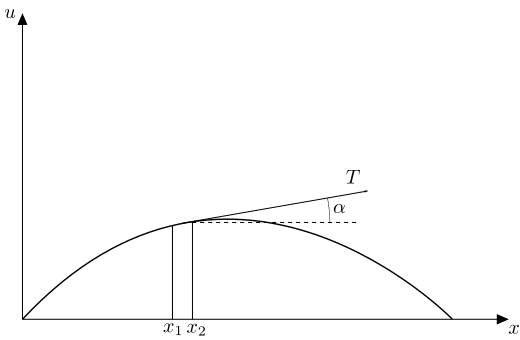
\includegraphics[scale=0.7]{string.pdf}  
		\caption{} \label{fig:string}
	\end{figure}

	Пусть $\rho$ -- линейная плотность струны, $a$ -- ускорение вдоль оси $x$:
	
	\[
		dm = \rho\, dx \quad a = \derp{x}{t}{2}
	\]
	Выделим бесконечно малый элемент струны и запишем II закон Ньютона:
	\[
		\rho \derp{x}{t}{2} dx = T_2 \cos \alpha_2 - T_1 \cos \alpha_1 = 0
	\]

	Пусть $\alpha_2, \alpha_1 \ll 1$, тогда $ \cos \alpha = 1 + O(\alpha^2). \quad T_2 = T_1 = T$\\
	Так как $\sum F_u \neq 0$, то 
	\[
		T_2 \sin \alpha_2 - T_1 \sin \alpha_1 = T (\alpha_2 - \alpha_1)
	\]
	Переходим к 
	\[
		\sin\alpha = \frac{\tg \alpha}{\sqrt{1 + \tg^2 \alpha}} = \frac{\derp{u}{x}{}}{\sqrt{1 + \left(\derp{u}{x}{}\right)^2}} \approx \derp{u}{x}{}
	\]
	\[
		\rho \derp{u}{t}{2} dx = T (\sin \alpha_2 - \sin \alpha_1) \approx  T \left( \derp{u}{x}{}\Bigl|_2 -  \derp{u}{x}{} \Bigl|_1 \right)
	\]
	Получаем уравнение  вида: 
	\[\rho \derp{u}{t}{2} = T \derp{u}{x}{2}\]
	В случае постоянной плотности $\rho = const$ это уравнение записывается в таком виде:\\
	\[\derp{u}{t}{2} = a^2 \derp{u}{x}{2}, \quad a = \sqrt{\frac{T}{\rho}}\]
 \newpage

	\subsection{Задача Коши для волнового уравнения.}	\label{que:8}
		Дифференциальные уравнения с обыкновенными и, тем более, с частными производными имеют, вообще говоря, бесчисленное множество решений. Поэтому в том случае, когда физическая задача приводится к уравнению с частными производными, для однозначной характеристики процесса необходимо к уравнению присоединить некоторые условия.\\

В случае дифференциального уравнения 2-го порядка решение может быть определено начальными условиями, т. е. заданием значений функций и её первой производной при <<\textit{начальном}>> значении аргумента (задача Коши).
	\[\derp{u}{t}{2} = a^2 \derp{u}{x}{2}, \quad x \in R,\, t = 0\]
Начальные условия
	\begin{align*}
		&t=0 \quad u(0, x) = f(x)\\
		&t=0 \quad \derp{u}{t}{} (0, x) = g(x)\\
	\end{align*}
Если струна закреплена, то должны выполняться <<\textit{граничные условия}>>\\
	\begin{itemize} \setlength{\itemindent}{10pt}
		\item[Задача \textbf{первого} типа]
		$\begin{aligned}
			&u(t, 0)  = \varphi(t)\\
			&u(t, l) = \xi(t)\\
		\end{aligned}$ -- заданный режим
		\item[Задача \textbf{второго} типа]
		$\begin{aligned}
			&\derp{u}{x}{}(t, 0) = \varphi(t)\\
			&\derp{u}{x}{}(t, l) = \xi(t)\\
		\end{aligned}$ -- заданная сила
	
		\item[Задача \textbf{третьего} типа]
		$\begin{aligned}
			&\derp{u}{x}{}(t, 0) = \alpha(u + \varphi)\\
			&\derp{u}{x}{}(t, l) = \beta(u + \xi)\\
		\end{aligned}$ -- упругое закрепление
	\end{itemize}


 \newpage

	\subsection{Редукция общей краевой задачи}\label{que:12}
		\setcounter{equation}{0}
При решении сложной задачи естественно стремиться свести её решение к решению более простых задач. С этой целью представим решение общей краевой задачи в виде суммы решений ряда частичных краевых задач.

Пусть $u_i(x, t) \quad (i = 1, 2, \ldots, n)$ -- функции, удовлетворяющие уравнениям
\begin{equation}
	\derp{u_i}{t}{2} = a^2 \derp{u_i}{x}{2} + f^i(x, t)
	\label{equ:Reduction1}
\end{equation}
при $0 < x < l, t > 0$ и дополнительным условиям
\begin{equation}
	\left.
	\begin{aligned}
		u_i(0, t) &= \mu_1^i(t),\\
		u_i(l, t) &= \mu_2^i(t);\\
		u_i (x, 0) & = \varphi^i(x),\\
		\derp{u_i}{t}{} (x, 0) &=\psi^i (x).
	\end{aligned}	
	\right\}
	\label{equ:Reduction2}
\end{equation}
Очевидно, что имеет место суперпозиция решений, т.е. функция
\begin{equation}
	u^{(0)}(x, t) = \sum\limits_{i = 1}^n u_i (x, t)
	\label{equ:Reduction3}
\end{equation}
удовлетворяет аналогичному уравнению с правой частью
\begin{equation}
	f^{(0)} (x, t) = \sum\limits_{i = 1}^n f^i (x, t)
	\label{equ:Reduction4}
\end{equation}
и дополнительным условиям, правые части которых суть функции
\begin{equation}
	\left.
	\begin{aligned}
		\mu_k^{(0)} = \sum\limits_{i = 1}^n \mu_k^i \quad (t) (l = 1, 2),\\
		\varphi^{(0)} (x) = \sum\limits_{i = 1}^n \varphi^i (x),\\
		\psi^{(0)} (x) = \sum\limits_{i = 1}^n \psi^i (x).
	\end{aligned}
	\right\}
	\label{equ:Reduction5}
\end{equation}
Указанный принцип суперпозиции относится, очевидно, не только к данной задаче, но и к любому линейному уравнению с линейными дополнительными условиями. \\

Решение общей краевой задачи 
\begin{equation}
	\left.
	\begin{aligned}
		u_{tt} = a^2 u_{xx} + f(x, y)\\
		(0 < x < l, t > 0);\\
		u(0, t) = \mu_1 (t),\\
		u(l, t) = \mu_2 (t);\\
		u(x, 0) = \varphi(x),\\
		u_t(x, 0) = \psi (x)
	\end{aligned}
	\right\}
	\label{equ:Reduction6}
\end{equation}
может быть представлено в виде суммы 
\[
	u(x, t) = u_1(x, t) + u_2 (x, t) + u_3 (x, t) + u_4 (x, t)
\]
где $u_1, u_2, u_3, u_4,$ -- решения следующих частных краевых задач:
\begin{equation}
	\left.
	\begin{aligned}
		u_1(0, t) &= 0, &u_2(0, t) &= \mu_1 (t), &u_3(0, t) &= 0,  &u_4(0, t) &= 0,\\
		u_1(l, t) &= 0; &u_2(l, t) &= 0; &u_3(l, t) &= \mu_2(t);  &u_4(l, t) &= 0;\\
		u_1(x, 0) &= \varphi(x), &u_2(x, 0) &= 0, &u_3(x, 0) &= 0,  &u_4(x, 0) &= 0,\\
		u_{1t}(x, 0) &= \psi(x); &u_{2t}(x, 0) &= 0; &u_{3t}(x, 0) &= 0;  &u_{4t}(x, 0) &= 0;\\
	\end{aligned}
	\right\}
	\label{equ:Reduction6}
\end{equation}

Аналогичная редукция может быть произведена и для предельных случаев общей краевой задачи.
\newpage

	\subsection{Метод распространяющихся волн}
		\subsubsection{Уравнение колебания бесконечной струны (Формула Даламбера)}
			\setcounter{equation}{0}
\begin{equation}
	\derp{u}{t}{2} = a^2 \derp{u}{x}{2} 
	\label{equ:equInfStringCauchy}
\end{equation}
Начальные условия 
\begin{alignat*}{1}
    u(x, 0) &= f(x)\\
    \derp{u}{t}{} (x, 0) &= g(x)
\end{alignat*}
Преобразуем это уравнение к каноническому виду, содержащему смешанную производную. Уравнение характеристик
\[
	dx^2 - a^2\, dt^2 = 0
\]
распадается на два уравнения:
\[
	dx - a\, dt = 0, \quad dx + a\, dt = 0.
\]
	Характеристиками уравненения являются две прямые:
\begin{align*}
	&\xi = x - at = C_1\\
	&\eta = x + at = C_2
\end{align*}
Приводим к каноническому виду
\begin{alignat*}{2}
	\derp{u}{t}{} &= a \derp{u}{\eta}{} - a \derp{u}{\xi}{} \quad &\derp{u}{t}{2} &= a^2 \derp{u}{\eta}{2} - 2 a^2 \derps{u}{\xi}{\eta} + a^2 \derp{u}{\xi}{2}\\
	\derp{u}{x}{} &=\derp{u}{\xi}{} + \derp{u}{\eta}{} \quad &\derp{u}{x}{2} &= \derp{u}{\xi}{2} + 2 \derps{u}{\xi}{\eta} + \derp{u}{\eta}{2}
\end{alignat*}
\[
	4 a^2 \derps{u}{\xi}{\eta} = 0
\]
В итоге уравнение колебаний струны преобразуется к виду:
\[
	\derps{u}{\xi}{\eta} = 0
\]
Найдём общий интеграл последнего уравнения:
\[
	\derp{u}{\eta}{} = \chi \quad \derp{\chi}{\xi}{} = 0
\]
\[
	\chi =V(\eta) \quad \derp{u}{\eta}{} = V(\eta)
\]
\[
	u(\xi, \eta)= \int\limits_{\eta_0}^{\eta} V(\tau) d \tau + \psi(\xi)
\]
\[
	u(\xi, \eta) = \varphi(\eta) + \psi (\xi)
\]
Функция
\begin{equation}
      u(x,t) = \varphi (x +at) + \psi (x - at)
	\label{equ:equCommonIntegral}
\end{equation}	

является общим интегралом уравнения \eqref{equ:equInfStringCauchy}.

Решение задачи называется корректным если оно существует, единственно и устойчиво.\\

\textbf{Существование}\\
	$\varphi(x +at)$ и $\psi(x - at)$ - должны допускать непрерывные частные производные.\\

\textbf{Единственность}\\
	Пусть $u(x, t) = \varphi (x + at) + \psi (x - at)$. Определим $f(x)$ и $g(x)$ таким образом, чтобы удовлетворялись начальные условия:
\begin{equation}
	u(x, 0) = \varphi (x) + \psi(x) = f(x)
	\label{equ:wave1}
\end{equation}
\[
	\derp{u}{t}{} (x, 0) = a \varphi'(x) - a \psi' (x) = g(x)
\]
Интегрируя второе равенство, получим:
\begin{equation}
	a \varphi(x) - a \psi(x) = \int\limits_{x_0}^{x} g(\tau) d \tau  + C
	\label{equ:wave2}
\end{equation}
где $x_0$ и $C$ - постоянные. Из \eqref{equ:wave1} и \eqref{equ:wave2} находим:
\[
	2 \varphi(x) = f(x) + \frac{1}{a} \int\limits_{x_0}^x g(\tau) d \tau + \frac{C}{2}
\]
\[
	2 \psi(x) = f(x) - \frac{1}{a} \int\limits_{x_0}^x g(\tau) d \tau - \frac{C}{2} 
\]
\begin{equation}
\begin{cases}
	 \varphi(x)  = \frac{1}{2} f(x) + \frac{1}{2a} \int\limits_{x_0}^x g(\tau) d \tau\\
	\psi(x) = \frac{1}{2} f(x) - \frac{1}{2a} \int\limits_{x_0}^x g(\tau) d \tau
\end{cases}
\label{equ:equWave3}
\end{equation}
Таким образом, мы определили функции $\varphi$ и $\xi$ через заданные $f$ и $g$, причём равенства \eqref{equ:equWave3} должны иметь место для любого значения аргумента\footnote{В формуле \eqref{equ:equCommonIntegral} функции $\varphi$ и $\xi$ определены неоднозначно. Если от $\varphi$ отнять, а к $\xi$ прибавить некоторую постоянную $C_1$, то $u$ не изменится. В формуле \eqref{equ:equWave3} постоянная $C$ не определяется через $\varphi$ и $\xi$, однако мы можем её отбросить, не меняя значения~$u$. При сложении $\varphi$ и $\xi$ слагаемые $\frac{C}{2}$ и $-\frac{C}{2}$  уничтожаются.}.
\begin{equation}
	u(x, t) = \frac{f(x + at) + f(x - at)}{2} + \frac{1}{2a} \int\limits_{x - at}^{x + at} g (\tau) d \tau
	\label{equ:equDalamber}
\end{equation}

Формулу \eqref{equ:equDalamber}, называемую \textit{формулой Даламбера}, мы получили, предполагая существование решения поставленной задачи. Эта формула доказывает единственность решения. Если бы существовало второе решение задачи \eqref{equ:equInfStringCauchy}, то оно представлялось бы формулой \eqref{equ:equDalamber} и совпадало бы с решением.\\

\textbf{Устойчивость}\\
Рассмотрим решение возмущённой задачи $\tilde u$:
\[
	\tilde u = f(x) + \varepsilon_1 \quad \derp{\tilde u}{t}{} (x, 0) = g(x) + \varepsilon_2
\]
Рассмотрим разность решений исходной и возмущённой задач
\[
	\abs{u(x, t) - \tilde u (x, t)} \leq \abs{\varepsilon_1} + \frac{1}{2a} \int\limits_{x - at}^{x + at} \varepsilon_2\, dt \leq \sigma(1 + t) \Rightarrow
\]
$\Rightarrow$ $\forall \varepsilon >0$ можно подобрать $\sigma: \sigma \leq \frac{\varepsilon}{1 + t}$\\
Следовательно решение устойчиво.
		


 \newpage	

		\subsubsection{Вывод уравнения Даламбера классическим способом}
			Рассмотрим задачу Коши для неоднородного уравнения колебаний
\[
	\derp{u}{t}{2} = a^2 \derp{u}{x}{2} + h(x, t)
\]
\[
		-\infty < x < \infty,	\quad	t > 0
\]
Начальные условия:
\begin{alignat*}{1}
	u(x, 0) &= f(x)\\
	\derp{u}{t}{} (x, 0) &= g(x)
\end{alignat*}

\begin{figure}[h!] 
	\centering 
	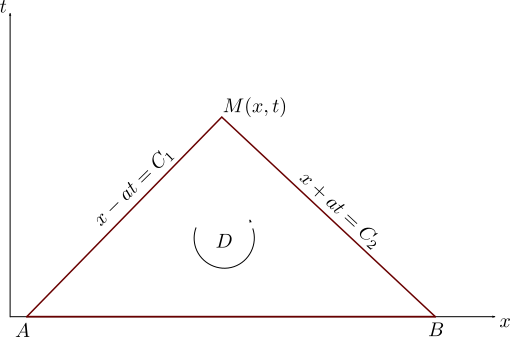
\includegraphics[width=0.6\textwidth]{figStringKoshi.pdf}
	\caption{Характеристический треугольник}
\end{figure}
Проинтегрируем обе части уравнения по области, заключённой внутри характеристического треугольника и разделим обе части на $2 a$.
\[
	\frac{1}{2a} \iint\limits_D \derp{u}{t}{2} dx dt = \frac{a}{2} \iint\limits_D \derp{u}{x}{2} dx dt + \frac{1}{2 a} \iint\limits_D h(x, t) dx dt
\]
Вспомним формулу Эйлера, которая помогает заменить интеграл по области на интеграл по границе.
По формуле Грина 
\[
	\iint\limits_D \derp{u}{t}{2} dxdt = - \oint\limits_{\partial D} \derp{u}{x}{} dt \qquad \iint\limits_D \derp{u}{x}{2} dx dt = \oint\limits_{\partial D} \derp{u}{x}{} dt
\]
\[
	- \oint_{\partial D} \derp{u}{t}{} = - \left[ \int\limits_A^B \derp{u}{t}{} dx + \int\limits_B^M \derp{u}{t}{} dx + \int\limits_M^A \derp{u}{t}{} dx \right] = 
\]
\[ 
	= - \int\limits_A^B \derp{u}{t}{} dx + a \int\limits_B^M \derp{u}{t}{} dt - a \int\limits_M^A \derp{u}{t}{} dt = 
\]
\[ 
	= - \int\limits_A^B \derp{u}{t}{} dx + 2 a u(M) - a u(A) - a u(B)
\]
\begin{multline*}
	\oint_{\partial D} \derp{u}{x}{} dt = \cancelto{0}{\int\limits_A^B \derp{u}{x}{} dt} + \int\limits_B^M \derp{u}{x}{} dt + \int\limits_M^A \derp{u}{x}{} dt = - \frac{1}{a} \int\limits_B^M \derp{u}{x}{} dx + \frac{1}{a} \int\limits_M^A \derp{u}{x}{} dx = \\ 
	=- \frac{2}{a} u(M) + \frac{(u(A) +u(B))}{a} = \frac{1}{2 a} \int\limits_A^B \derp{u}{t}{} dx + u(m) - \frac{u(B) +u(A)}{2} =\\=
	 - u(M) + \frac{u(B)+u(A)}{2}  + \frac{1}{2a} \iint\limits_D h(x, t) dx dt
\end{multline*}
\[
	2 u(M) = \frac{1}{2a} \int\limits_A^B \derp{u}{t}{} dx + u(A) +u(B) + \frac{1}{2a} \iint\limits_D h(x, t) dx dt
\]
\[
	x_m - at_m = C_1 = x - at \Rightarrow x_A = x_m - at_m
\]
\[
	x_m + at_m = C_2 = x + at \Rightarrow x_B = x_m - at_m
\]
Получим:
\[
	u(M) = \frac{u(x_m +at_m) + u(x_m - a t_m)}{2} + \frac{1}{2a} \int\limits_{x_m - at_m}^{x_m + a t_m} g(\xi) d \xi + \frac{1}{2a} \iint\limits_D h(x, t) dx dt
\]



 \newpage

		\subsubsection{Полубесконечная струна и метод продолжений}\label{que:9}
			Рассмотрим задачу о распространении волн на полуограниченной прямой $x \geqslant 0$. Эта задача имеет особенно важное значение при изучении процессов отражения волн от конца и ставится следующим образом:\\

\textit{найти решение уравнения колебаний}
\[
	\derp{u}{t}{2} = a^2\, \derp{u}{x}{2} 
\]
\textit{при $0 < x < \infty$,\quad $t > 0$,}\\
\textit{удовлетворяющее граничному условию}
\[
	u(0, t) = \mu(t) \:(\mbox{или}\: \derp{u}{x}{}(0, t) = \nu(t)) \quad t \geqslant 0
\]
\textit{и начальным условиям}
\begin{alignat*}{1}
	u(x, 0) &= f(x)\\
	\derp{u}{t}{}(x, 0) &= g(x)
\end{alignat*}
$0 \leqslant x < \infty$.\\

Отметим две леммы о свойствах решений уравнений колебаний, определённых на бесконечной прямой.
\begin{enumerate}
	\item \textit{Если начальные данные в задаче о распространении колебаний на неограниченной прямой} (\textit{задача} \eqref{equ:equInfStringCauchy})  \textit{являются нечётными функциями относительно некоторой точки $x_0$, то соответствующее решение в этой точке $x_0$ равно нулю.}
	\item \textit{Если начальные данные в задаче о распространении колебаний на неограниченной прямой}  (\textit{задача} \eqref{equ:equInfStringCauchy}) \textit{являются чётными функциями относительно некоторой точки $x_0$, то производная по $x$ соответствующего решения в этой точке равна нулю.}
\end{enumerate}


Примем $x_0$ за начало координат, $x_0 = 0$. В этом случае условия нечётности начальных данных ($f(x)$ и $g(x)$ - нечётные) запишутся в виде 
\[
	f(x) = - f(-x); \quad g(x) = - g(- x).
\]
Функция $u(x, t)$, определяемая формулой \eqref{equ:equDalamber}, при $x = 0$ и $t > 0$ равна
\[
	u(0, t) = \frac{f(at) +f(-at)}{2} + \frac{1}{2a} \int\limits_{-at}^{at} g(\xi) d\xi = 0
\]
так как первое слагаемое равно нулю в силу нечётности $f(x)$, а второе равно нулю, поскольку интеграл от нечётной функции в пределах, симметричных относительно начала координат, всегда равен нулю.\\

Аналогично для второй леммы. Условия чётности начальных данных имеют вид
\[
	f(x) = f(-x); \quad g(x) = g(- x).
\]
Заметим, что производная чётной функции является функцией нечётной
\[
	\varphi'(x) = - \varphi '(- x)
\]
Из формулы \eqref{equ:equDalamber} следует:
\[
	u_x(0, t) = \frac{f'(at) + f'(-at)}{2}  + \frac{1}{2a} [g(at) - g(-at)] = 0, \quad t > 0,
\]
так как первое слагаемое равно нулю в силу нечётности $f'(x)$, а второе - в силу чётности $g(x)$.\\
Рассмотрим граничное условие
\[
	u(0, t) = 0, \quad t > 0
\]
Функцию $f(x)$ можно продолжить  нечётным образом:
\[
	f_1(x) = sgn(x) \cdot f(\abs{x})
\]
Аналогично для 
\[
    g_1(x) = sgn (x) \cdot g(\abs{x})
\]

\begin{enumerate}
	\item $x - at > 0; \quad$ -- решение записывается в обычном виде\\ (в области $t < \frac{x}{a}$ влияние граничных условий не сказывается и выражение для $u(x, t)$ совпадает с решением \eqref{equ:equDalamber} для бесконечной прямой.)\\
	\item $x - at < 0; \quad  x > 0,\quad  t > \frac{x}{a}$
\end{enumerate}
Получим решение уравнения колебаний
\begin{multline*}
	u(x, t) = \frac{f_1(x + at) + f_1(x - at)}{2} + \frac{1}{2a} \int\limits_0^{x +at} g_1(\xi)\, d \xi + \frac{1}{2 a} \int\limits_{x - at}^0 g_1 (\xi )\, d\xi =\\= [-z = \xi \quad -dz = d\xi ] 
	= \frac{f_1(x + at) + f_1(x - at)}{2} +  \frac{1}{2a} \int\limits_0^{x +at} g_1(\xi)\, d \xi + \frac{1}{2 a} \int\limits_0^{at -x} g_1 (z )\, dz
\end{multline*}
или
\[
	u(x, t) = \frac{f_1(x + at) + f_1(x - at)}{2} + \frac{1}{2a} \int\limits_{x-at}^{x+at} g_1(\xi)\, d\xi
\]
Сформулируем метод продолжений:\\

\textit{Для решения задачи на полубесконечной прямой с граничным условием $u(0, t) = 0$ начальные данные надо продолжить на всю прямую нечётно.}

\textit{Для решения задачи на полубесконечной прямой с граничным условием $u_x(0, t) = 0$ начальные данные надо продолжить на всю прямую чётно.}\\


\newpage


	\subsection{Метод Фурье для уравнения колебания струны} \label{que:10}
		\setcounter{equation}{0}
Метод разделения переменных или метод Фурье, является одним из наиболее распространённых методов решения уравнений с частными производными. Изложение этого метода проведём для задачи о колебаниях струны, закреплённой на концах.\\
\begin{equation}
	\derp{u}{t}{2} = a^2\, \derp{u}{x}{2}
	\label{equ:equCauchyWaveFourier}
\end{equation}
Начальные условия: 
\begin{align}
	u(x, 0) = f(x)\\
	u_t(x, 0) = g (x)
	\label{equ:equCauchyWaveFourierN}
\end{align}
Граничные условия:
\begin{align}
	u(0, t) = 0, \quad u(l, t) = 0
	\label{equ:equCauchyWaveFourierGr}
\end{align}
Уравнение \eqref{equ:equCauchyWaveFourier} линейно и однородно, поэтому сумма частных решений также является решением этого уравнения. Имея достаточно большое количество частных решений, можно попытаться при помощи суммирования их с некоторыми коэффициентами найти искомое решение. \\

Поставим основную вспомогательную задачу:\\
\textit{найти решение уравнения \eqref{equ:equCauchyWaveFourier} не тождественное нулю, удовлетворяющее однородным граничным условиям}
\begin{align*}
		u(0, t) = 0\\
		u(l, t) = 0
\end{align*}
\textit{и представимое в виде произведения }
\begin{equation}
	u(x,t)= X(x) T(t)
	\label{equ:equWaveFourierSolveView}
\end{equation}
\textit{где $X(x)$ -- функция только переменного $x$, $T(t)$ -- функция только переменного $t$.}\\

Подставляя предполагаемую форму решения \eqref{equ:equWaveFourierSolveView} в уравнение \eqref{equ:equCauchyWaveFourier}, получим:
\[
	X''T = \frac{1}{a^2} T''X
\]
после деления на $XT$
\[
	\frac{X''}{X} = \frac{1}{a^2} \frac{T''}{T} = - k^2\
\]
Из этого соотношения получаем обыкновенные дифференциальные уравнения для определения функций $X(x)$ и $T(x)$
\begin{alignat}{2} \label{equ:equCauchy1}
	X''(x) + k X(x) &= 0, \quad &X(x) &\not\equiv 0\\
	T''(t) + a^2 k T(t) &= 0, \quad &T(t) &\not\equiv 0
	\label{equ:equCauchy2}
\end{alignat}

Приходим к задаче о собственных значениях (задаче \textit{Штурма---Лиувилля}).
\[
	\begin{cases}
		X'' + kX = 0\\
		X(0) = X(l) = 0
	\end{cases}
\]
При $k < 0$ и $k = 0$ задача не имеет нетривиальных решений. Это можно проверить найдя решения этих двух случаев, общий вид которых $X(x) = C_1 e^{\sqrt{-k}x} + C_2 e^{-\sqrt{-k}x}$ и $X(x) = C_1 x + C_2$ соответственно.
Рассмотрим случай при $k > 0$.

Общее решение ищется в виде
\[
	X_k = C_{1k}^* \cos kx + C_{2k}^* \sin k x
\]
Граничные уловия дают:
\[
	X(0) = 0 \Rightarrow C_1^* = 0
\]
\[
	X(l) = 0 \Rightarrow C_{2k}^*\sin k l = 0
\]
\[
	k l=\pi n \Rightarrow k_n=\pi\frac{n}{l}
\]
$k_n$ -- cобственные числа.

Этим собственным числам соответствую собственные функции ($n \in N$)
\[
	X_n= C_{2n}^* \sin \frac{\pi n}{l} x
\]
Этим же значениям $k_n$ соответствуют решения уравнения \eqref{equ:equCauchy2}
\[
	T_n = A_k\cos \frac{a\pi k}{l} t + B_k \sin\frac{a\pi k}{l} t,
\] 
где $A_k$ и $B_k$ -- произвольные постоянные.
\begin{align*}
	&A_n C_{2n}^* =C_{1n}\\
	&B_n C_{2n}^* = C_{2n}
\end{align*}
Функции
\[
	u_n (x, t) = \left(C_{1n} \cos \frac{a \pi n}{l} t + C_{2n} \sin \frac{a \pi n}{l} t \right) \sin\frac{\pi n}{l} x
\]
являются частными решениями уравнения \eqref{equ:equCauchyWaveFourier}, удовлетворяющими граничным условиям \eqref{equ:equCauchyWaveFourierGr}. Эти решения могут удовлетворить начальным условиям нашей исходной задачи только для частных случаев начальных функций $f(x)$ и $g(x)$. \\

В силу линейности и однородности уравнения \eqref{equ:equCauchyWaveFourier} сумма частных решений
\begin{equation}
	u(x, t) = \sum\limits_{n = 1}^{\infty} u_n (x, t) = \sum\limits_{n = 1}^{\infty} \left(C_{1n} \cos \frac{a \pi n}{l} t + C_{2n} \sin \frac{a \pi n}{l} t \right) \sin\frac{\pi n}{l} x
	\label{equ:equUniSolveFourWave}
\end{equation}
также удовлетворяет этому уравнению и граничным условиям. 

Начальные условия позволяют определить $C_{1n}$ и $C_{2n}$. Потребуем, чтобы функция \eqref{equ:equUniSolveFourWave} удовлетворяла условиям \eqref{equ:equCauchyWaveFourierN}:
\begin{equation}
	\left.
	\begin{aligned}
		&u(x, 0) = f(x) = \sum\limits_{n = 1}^{\infty}  u_n(x, 0) = \sum\limits_{n = 1}^{\infty} C_{1n} \sin \frac{\pi n}{l} \, x,\\
		&u_t(x, 0) = g(x) = \sum\limits_{n = 1}^{\infty}  \derp{u_n}{t}{}(x, 0) = \sum\limits_{n = 1}^{\infty} \frac{\pi n}{l} a C_{2n} \sin \frac{\pi n}{l} \, x.
	\end{aligned}
	\right\}
	\label{equ:equwaveFourier1}
\end{equation}

Из теории рядов Фурье известно, что произвольная кусочно-непрерывная и кусочно-дифференциируемая функция $\varphi(x)$, заданная в промежутке $0 \leqslant x \leqslant l$, разлагается в ряд Фурье
\[
	\varphi(x) = \sum\limits_{n = 1}^\infty b_n \sin \frac{\pi n}{l} x,
\]
где 
\[
	b_n = \frac{2}{l} \int\limits_0^l f(\xi) \sin \frac{\pi n}{l}\xi \, d\xi
\]

Найдём коэффициенты $C_{1n}$
\[
	 C_{1n} = \frac{2}{l} \int\limits_0^l f(x) \sin \frac{n \pi}{l} x\, dx
\]
Коэффициенты $C_{2n}$ находят из 2-го условия $\derp{u}{t}{} |_{t = 0} = g(x)$\\
\[
	g(x) = \left. \sum\limits_{n = 1}^{\infty}\left(C_{2n}\cos \frac{a \pi n}{l} t + C_{1n} \sin \frac{a \pi n}{l} t \right) \frac{a \pi n}{l} \sin \frac{\pi n}{l} x \right|_{t = 0}
\]
\[
	g(x) = \sum\limits_{n = 1}^{\infty} C_{2n} \frac{a \pi n}{l} \sin \frac{\pi n}{l} x
\]
\[
	\frac{2}{l} \int\limits_0^l g(x) \sin \frac{\pi n}{l} x dx = \frac{a \pi n}{l} C_{2n} 
\]
\[
	C_{2n} = \frac{2}{a \pi n} \int\limits_0^l g(x) \sin \frac{\pi n}{l} x\, dx
\]
В итоге
\begin{align*}
	&C_{1n} = \frac{2}{l} \int\limits_0^l f(x) \sin \frac{n \pi}{l} x\, dx\\
	&C_{2n} = \frac{2}{a \pi n} \int\limits_0^l g(x) \sin \frac{\pi n}{l} x\, dx
\end{align*}\\
Проверим, совпадает ли данное решение с решением Д'Аламбера.

\[	
	u(x, t) = \frac{f(x + at) + f(x - at)}{2} + \frac{1}{2a} \int\limits_{x - at}^{x + at} g(\xi)\, d \xi
\]
\[
	f(x) = \sum\limits_{n = 1}^{\infty} C_{1n} \sin \frac{\pi n}{l} x \quad g(x) = \sum\limits_{n = 1}^{\infty} C_{2n} \frac{a \pi n}{l} \sin \frac{\pi n}{l} x\
\]
\begin{multline*}
	u(x,t) = \frac{1}{2} \left[ \sum\limits_{n = 1}^{\infty} C_{1n} \sin \frac{\pi n}{l} (x - at) + \sum\limits_{n = 1}^{\infty} C_{1n} \sin \frac{\pi n}{l} (x + at)\right] + \frac{1}{2a} \int\limits_{x - at}^{x + at} \sum\limits_{n = 1}^{\infty} C_{2n} \frac{a \pi n}{l} \sin \frac{\pi n}{l} \xi \, d \xi =\\
	= \sum\limits_{n = 1}^{\infty} C_{1n} \sin \frac{\pi n}{l} x \cos at \frac{\pi n}{l} +\frac{\pi}{a 2 l} \sum\limits_{n = 1}^{\infty} \int\limits_{x - at}^{x + at} C_{2n} n \sin\frac{\pi n}{l}\xi \, d \xi =\\
	=\left. \sum\limits_{n = 1}^{\infty}C_{1n} \sin \frac{\pi n}{l} x \cos \frac{a \pi n}{l} t - \frac{a \pi}{a 2 l} \sum\limits_{n = 1}^{\infty} C_{2n} \frac{l}{\pi} \cos \frac{\pi n}{l} \right|_{x - at}^{x + at} =\\
	= \sum\limits_{n = 1}^{\infty} \left( C_{1n}\sin \frac{\pi n}{l} x \cos\frac{a \pi n}{l} t + C_{2n} \sin \frac{\pi n}{l} x \cdot \sin \frac{\pi n a}{l} t\right) =\\
	= \sum\limits_{n = 1}^{\infty} \left(C_{1n} \cos \frac{\pi n a}{l} t +  C_{2n} \sin \frac{\pi n a}{l} t \right) \sin \frac{\pi n}{l} x
\end{multline*}
Таким образом убедились в правильности решения. \newpage

	\subsection{Метод Фурье для неоднородного уравнения колебания струны} \label{que:11}
		Рассмотрим неоднородное уравнение колебаний
\begin{equation}
	\derp{u}{t}{2} = a^2 \derp{u}{x}{2} + f(x, t), \quad a^2 = \frac{k}{\rho}, \quad 0 < x < l
	\label{equ:FourierNonordinary1}
\end{equation}
с начальными условиями
\begin{equation}
	\left.
	\begin{aligned}
		u(x, 0) &= \varphi(x),\\
		u_t(x, 0) &= \psi(x),
	\end{aligned}
	\right\} \quad 0 \leqslant x \leqslant l
	\label{equ:FourierNonordinary2}
\end{equation}
и однородными граничными условиями
\begin{equation}
	\left.
	\begin{aligned}
		u(0, t) &= 0,\\
		u(l, t) &= 0,
	\end{aligned}
	\right\} \quad t > 0.
	\label{equ:FourierNonordinary3}
\end{equation}
Будем искать решение задачи в виде разложения в ряд Фурье по $x$
\begin{equation}
	u(x, t) = \sum\limits_{n = 1}^{\infty} u_n(t) \sin \frac{\pi n}{l}x,
	\label{equ:FourierNonordinary4}
\end{equation}
рассматривая при этом $t$ как параметр. Для нахождения $u(x, t)$ надо определить функцию $u_n(t)$. Представим функцию $f(x, y)$ и начальные условия в виде рядов Фурье:
\begin{equation}
	\left.
	\begin{aligned}
		f(x, t) &= \sum\limits_{n = 1}^{\infty} f_n (t) \sin \frac{\pi n}{l} x, &f_n(t) &= \frac{2}{l} \int\limits_0^l f(\xi, t) \sin \frac{\pi n}{l} \xi\, d \xi;\\
		\varphi(x) &= \sum\limits_{n = 1}^{\infty} \varphi_n \sin \frac{\pi n}{l}x, &\varphi_n &= \frac{2}{l} \int\limits_0^l \varphi(\xi) \sin \frac{\pi n}{l} \xi \, d\xi\\
		\psi(x) &= \sum\limits_{n = 1}^{\infty} \psi_n \sin \frac{\pi n}{l}x, &\psi_n &= \frac{2}{l} \int\limits_0^l \psi(\xi) \sin \frac{\pi n}{l} \xi \, d\xi
	\end{aligned}
	\right\} 
	\label{equ:FourierNonordinary5}
\end{equation}
Подставляя предполагаемую форму решения \eqref{equ:FourierNonordinary4} в исходное уравнение  \eqref{equ:FourierNonordinary1}
\[
	\sum\limits_{n = 1}^\infty \sin \frac{\pi n}{l} x \left\{- a^2 \left(\frac{\pi n}{l} \right)^2 u_n(t) - \ddot u_n (t) + f_n (t) \right\} = 0,
\]
видим, что оно будет удовлетворено, если все коэффициенты разложения равны нулю, т.е.
\begin{equation}
	\ddot u_n(t) + \left(\frac{\pi n}{l} \right)^2 a^2 u_n (t) = f_n (t).
	\label{equ:FourierNonordinary6}
\end{equation}

Для определения $u_n(t)$ мы получили обыкновенное дифференциальное уравнение с постоянными коэффициентами. Начальные условия дают:
\begin{align*}
	u(x, 0) = \varphi(x) = \sum\limits_{n = 1}^\infty u_n(0) \sin \frac{\pi n}{l} x = \sum\limits_{n = 1}^\infty \varphi_n \sin \frac{\pi n}{l} x,\\
	u_t(x, 0) = \psi(x) = \sum\limits_{n = 1}^\infty \dot u_n(0) \sin \frac{\pi n}{l} x = \sum\limits_{n = 1}^\infty \psi_n \sin \frac{\pi n}{l} x,
\end{align*}
откуда следует:
\begin{equation}
	\left.
	\begin{aligned}
		u_n(0) = \varphi_n,\\
		\dot u_n(0) = \psi_n.
	\end{aligned}
	\right\}
	\label{equ:FourierNonordinary7}
\end{equation}

Эти дополнительные условия полностью определяют решение уравнения \eqref{equ:FourierNonordinary6}. Функцию $u_n(t)$ можно представить в виде
\[
	u_n(t) = u_n^{(\mathrm{I})} (t) + u_n^{(\mathrm{II})} (t) 
\]
где
\begin{equation}
	u_n^{(\mathrm{I})} (t) = \frac{1}{\pi n a} \int\limits_0^t \sin \frac{\pi n}{l} a (t - \tau) \cdot f_n (\tau)\, d\tau
	\label{equ:FourierNonordinary8}
\end{equation}
есть решение неоднородного уравнения с нулевыми начальными условиями и 
\begin{equation}
	u_n^{(\mathrm{II})} (t) = \varphi_n \cos \frac{\pi n}{l} at + \frac{1}{\pi n a}\psi_n \sin \frac{\pi n}{l} a t
	\label{equ:FourierNonordinary9}
\end{equation}
--- решение однородного уравнения с заданными начальными условиями. Таким образом, искомое решение запишется в виде
\begin{align*}
	&u(x, t) = \sum\limits_{n = 1}^\infty \frac{1}{\pi n a} \int\limits_0^t \sin \frac{\pi n}{l} a (t - \tau) \sin \frac{\pi n}{l}x \cdot f_n(\tau)\, d\tau + \\
	&\phantom{u(x, t) =} + \int\limits_{n = 1}^\infty \left(\varphi_n \cos \frac{\pi n}{l} a t + \frac{1}{\pi n a} \psi_n \sin \frac{\pi n}{l} a t \right) \sin \frac{\pi n}{l}x.
\end{align*}

Вторая сумма представляет решение задачи о свободных колебаниях струны при заданных начальных условиях и была решена ранее. Обратимся к первой сумме, представляющей вынужденные колебания струны под действием внешней силы при нулевых начальных условиях. Пользуясь выражением \eqref{equ:FourierNonordinary5} для $f_n(t)$, находим:
\begin{align*}
	u_n^{(\mathrm{I})} (x, t) &= \int\limits_0^t \int\limits_0^l \left\{\frac{2}{l} \sum\limits_{n = 1}^\infty \frac{l}{\pi n a} \sin \frac{\pi n}{l} a(t - \tau) \sin \frac{\pi n}{l} x \sin \frac{\pi n}{l} \xi \right\} f(\xi, \tau)\, d\xi d\tau =\\
	&=\int\limits_0^t \int\limits_0^l G(x, \xi, t - \tau) f(\xi, \tau)\, d\xi d\tau,
\end{align*}
где 
\[
	G(x, \xi, t - \tau) = \frac{2}{\pi a} \sum\limits_{n = 1}^\infty \frac{1}{n} \sin \frac{\pi n}{l} a(t - \tau) \sin \frac{\pi n}{l} x \sin \frac{\pi n}{l} \xi.
\]
 \newpage

	\subsection{Пример некорректно поставленной задачи}
		Рассмотрим пример некорректно поставленной задачи:\\
\[
	\derp{u}{t}{2} + \derp{u}{x}{2} = 0
\]
\[
	u(x, 0) =  \frac{\sin \lambda x}{\lambda}, \quad \derp{u}{t}{} = 0
\]

Решением является
\[
	u(x, t) = \frac{1}{\lambda} \sin \lambda x \ch \lambda t
\]

\[
	\derp{u}{t}{2} = \lambda \sin \lambda x \ch \lambda t \quad \derp{u}{x}{2} = - \lambda \sin \lambda x \ch \lambda t
\]
\[
	u(x, 0) = \frac{\sin \lambda x}{\lambda} \quad \derp{u}{t}{} (x, 0) = \sin \lambda x\sh 0 = 0
\]
\[
	\lambda \to \infty \Rightarrow u(x, 0) \to 0
\]
Тогда, $u_1 = 0$ - решение уравнения:\\
\[
	\abs{u(x, 0)- u_1(x,0)} < \sigma_1
\]
\[
	\abs{\derp{u}{t}{} (x, 0) - \derp{u_1}{t}{}} < \sigma_2
\]
\[
	\abs{u(x, t) - u_1(x, t)} = \abs{\frac{1}{\lambda} \sin \lambda x \frac{e^{\lambda t} + e ^{- \lambda t}}{2}}
\]
-- сколь угодно большое число.

Следовательно решение является неустойчивым и, значит,  задача поставлена некорректно.\newpage

	\subsection{Метод Римана решения волновых уравнений}
		Установим некоторые вспомогательные формулы, нужные для представления решений краевых задач в интегральной форме. Пусть
\[
	L[u] = \derps{u}{x}{y} + a(x, y) \derp{u}{x}{} + b(x, y) \derp{u}{y}{} + c(x, y) u 
\]
-- линейный дифференциальный оператор, соответствующий уравнению гиперболического типа.\\
Характеристиками уравнения являются $y = C_1$ и $x = C_2$.
Начальные условия будем задавать на кривой $y = g(x)\quad (x = \eta(y))$.

\begin{wrapfigure}[0]{r}{0.35\textwidth}
	\centering
	\includegraphics[width=0.2\textwidth]{fighyperriman.pdf}
\end{wrapfigure}
\begin{minipage}[t]{0.7\textwidth}
\begin{align*}
	&u|_{y = g} = g(x)\\
	&\left.\derp{u}{y}{}\right| =  \psi(x)
\end{align*}
\begin{align*}
	&L[u] =  \derps{u}{x}{y} + a(x, y) \derp{u}{x}{} + b(x, y) \derp{u}{y}{} + c(x, y) u \\
	&L^*[v] = \derps{v}{x}{y} - \derp{}{x}{} \left(a v \right) - \derp{}{y}{} \left(b v \right) + c  v\\
\end{align*}
\end{minipage}\\


\begin{multline*}
	vL[u] - u L^*[v] = v \derps{u}{x}{y} - u \derps{v}{x}{y} + a v \derp{u}{x}{}  + u \derp{}{x}{} \left(a v \right) + b v \derp{u}{y}{} + u \left(b v \right) =\\
	= \frac{1}{2} \derp{}{x}{} \left(v \derp{u}{y}{} \right) - \frac{1}{2} \derp{v}{x}{} \derp{u}{y}{} + \frac{1}{2} \derp{}{y}{} \left(v \derp{u}{x}{} \right) - \frac{1}{2} \derp{v}{y}{} \derp{u}{x}{} - \frac{1}{2} \derp{}{x}{} \left(u \derp{v}{y}{} \right) + \frac{1}{2} \derp{u}{x}{} \derp{v}{y}{} - \frac{1}{2} \derp{}{y}{} \left(u \derp{v}{x}{} \right) + \frac{1}{2} \derp{u}{y}{} \derp{v}{x}{} = \\
	= \frac{1}{2} \derp{}{x}{} \left(v \derp{u}{y}{} - u \derp{v}{y}{} + 2 a u v \right) + \frac{1}{2} \derp{}{y}{} \left(v \derp{u}{x}{} - u \derp{v}{x}{} + 2 b u v \right)
\end{multline*}
Пришли к \textit{дивергентному виду}.

Из этого следует, что $L^*$ -- сопряжённый оператор.

\[
	v L[u] - u L^*[v] = \frac{1}{2} \derp{}{x}{} \left( v \derp{u}{y}{} - u \derp{v}{y}{} + 2 auv \right) + \frac{1}{2} \derp{}{y}{}\left(v \derp{u}{x}{} - u \derp{v}{x}{} + 2 b u v\right)
\]
\begin{multline*}
	\iint\limits_D\left[v L[u] - u L^* [v] \right] = \frac{1}{2} \oint \left[ \left(v \derp{u}{y}{} - u \derp{v}{y}{}  + 2 au v\right)\, dy - \left(v \derp{u}{x}{} - u \derp{v}{x}{} + 2 b u v \right)\, dx \right] = \\
	= - \frac{1}{2} \int\limits_A^B \left(v \derp{u}{x}{} - u \derp{v}{x}{} + 2 buv\right)\, dx + \frac{1}{2} \int\limits_B^C \left(v \derp{u}{y}{} - u \derp{v}{y}{} + 2 auv\right)\, dy +{}\\+ \frac{1}{2} \int\limits_C^A \left[\left(v \derp{u}{y}{} - u \derp{v}{y}{} + 2 u v a\right)\, dy + \left(u \derp{v}{x}{} - v \derp{u}{x}{} + 2 b u v \right)\, dx\right] =\\
	= - \frac{1}{2} uv \Big|_A^B + \frac{1}{2} \int\limits_A^B u \left( 2 \derp{v}{x}{} - 2 bv \right)\, dx + \frac{1}{2} uv \Big|_B^C + \frac{1}{2} \int\limits_B^C u \left(-2 \derp{v}{y}{} \right)\, dy + \frac{1}{2} \int\limits_A^C \left[\ldots \right]\, dx dy
\end{multline*}
Потребуем $\derp{v}{x}{} - bv = 0 \big|_{y = Y_0}, \quad \derp{v}{y}{} - a v = 0 \big|_{x = X_0}$\\

\begin{equation}
	v = C e^{\int\limits_{x_0}^x b \,dx} \qquad v = C e^{\int\limits_{y_0}^y a \,dy}
	\label{equ:equRiman}
\end{equation}
где $C = 1$.\\
$v(x, y, x_0, y_0)$ -- \textit{функция Римана}.\\

Для функции Римана должно выполняться $v(x_0, y_0, x_0, y_0) = 1$ и она должна удовлетворять $L^*(v) = 0$. Известно, что $L[u] = f(x, y)$, тогда
\[
	vL[u] = v f(x, y)
\]
Тогда для интеграл принимает вид
\[
	\iint\limits_D v f(x, y)\, dx dy = \frac{1}{2} \left(uv\Big|_A - u v\Big|_B \right) + \frac{1}{2} \left(uv\Big|_C - uv \Big|_B \right) + \frac{1}{2} \int\limits_C^A \left[ \ldots \right]\, dx dy
\]
Для
\[
	B= (x_0, y_0) \Rightarrow v\Big|_B = 1,
\]
мы получаем
\[
	v u(B) = \frac{uv\big|_A + u v \big|_B}{2} + \frac{1}{2} \int\limits_C^A \left[\left(v \derp{u}{y}{} - u \derp{v}{y}{}  + 2 auv\right)\, dy + \left(u \derp{v}{x}{} - v \derp{u}{x}{} + 2 bu v \right)\, dx \right] - \iint\limits_D f(x,y)\, dx dy
\]
%Двойной интеграл от разности $vl[u] - u l^*[v]$ по некоторой области $g$, ограниченной кусочно-%гладким контуром $c$, равен 
%\[
%	\iint\limits_g (v l[u] - u l^*[v] )\, d\xi \, d\eta = \int\limits_c (h\, d\eta - k\, d\xi)
%\]
%где $u$ и $v$ - произвольные дважды дифференциируемые функции(двумерная формула Грина).
\newpage
\begin{example}{Телеграфное уравнение}
\[
	\derp{u}{x}{2} = LC \derp{u}{t}{2} + \left(RC + LG \right) \derp{u}{t}{} + RGu
\]
Начальные условия ($t = 0$): 
\begin{align*}
	u &= f(x);\\
	\derp{u}{t}{} &= g(x)
\end{align*}
\[
		a_0 = LC, \quad RC - LG = 2 b_0, \quad RG = C_0
\]
\[
	\derp{u}{x}{2} = a_0 \derp{u}{t}{2} + 2 b_0 \derp{u}{t}{} + C_0 u
\]
Будем искать $u$ в виде 
\[
	u = e^{- \frac{b_0}{a_0}t} \cdot w(x, t)
\]
\begin{align*}
	&\derp{u}{x}{} = e^{- \frac{b_0}{a_0}t} \derp{w}{x}{} &\derp{u}{x}{2} = e^{- \frac{b_0}{a_0}t} \derp{w}{x}{2}\\
	&\derp{u}{t}{} = - \frac{b_0}{a_0} e^{- \frac{b_0}{a_0} t} w(x,t) + e^{- \frac{b_0}{a_0}t} \derp{w}{t}{}
	&\derp{u}{t}{2} = \frac{b_0^2}{a_0^2} e^{-\frac{b_0}{a_0}} w(x, t) - 2 \frac{b_0}{a_0} \derp{w}{t}{} e^{- \frac{b_0}{a_0}t} + e^{- \frac{b_0}{a_0}} \derp{w}{t}{2}
\end{align*}

\[
	\derp{w}{x}{2} = a_0 \derp{w}{t}{2} - \cancel{2 b_0 \derp{w}{t}{}} + \cancel{\frac{b_0^2}{a_0} w} - \cancel{2} \frac{b_0^2}{a_0} w + \cancel{2 b_0 \derp{w}{t}{}} + c_0 w
\]\\
\[
	\begin{cases}
		\displaystyle\derp{w}{x}{2} = a_0 \derp{w}{t}{2} + \left(c_0 - \frac{b_0^2}{a_0} \right) w\\
		t = 0 \quad w(x, 0) = f(x) \quad \derp{w}{t}{} = g(x) + \frac{b_0}{a_0} f(x)
	\end{cases}
\]
\[	
	\derp{w}{t}{2} = \underbrace{\frac{1}{a_0}}_{a^2} \derp{w}{x}{2} + \underbrace{\frac{b_0 - a_0 c_0}{a_0^2}}_{b^2} w
\]
Итак
\[
	\begin{cases}
		\displaystyle\derp{w}{x}{2} = a^2 \derp{w}{t}{2} +b^2 w\\
		t = 0 \quad w(x, 0) = f(x) \quad \derp{w}{t}{} = g(x) + \frac{b_0}{a_0} f(x)
	\end{cases}
\]\\

Вернёмся к характеристическим переменным:
\[
	\begin{cases}
		\xi = \frac{b}{a}(x + at)\\
		\eta = \frac{b}{a}(x - at)
	\end{cases}
	\qquad
	\begin{cases}
		t = \frac{\xi - \eta}{2b}\\
		x = \frac{(\xi + \eta)}{2}\frac{a}{b}
	\end{cases}
\]
тогда 
\begin{align*}
	&\derp{w}{t}{} = \left(\derp{w}{\xi}{} - \derp{w}{\eta}{} \right)b &\derp{w}{t}{2} = b^2 \left(\derp{w}{\xi}{2} - 2 \derps{w}{\xi}{\eta} + \derp{w}{\eta}{2} \right)\\
	&\derp{w}{t}{} = \frac{b}{a} \left(\derp{w}{\xi}{}  + \derp{w}{\eta}{}\right)
	&\derp{w}{x}{2} = \frac{b^2}{a^2} \left(\derp{w}{\xi}{2} + 2 \derps{w}{\xi}{\eta} + \derp{w}{\eta}{2} \right)
\end{align*}
В итоге
\[
	4 b^2 \derps{w}{\xi}{\eta} + b^2 w = 0
\]
Следовательно
\[
	\derps{w}{\xi}{\eta} = - \frac{w}{4}
\]
\end{example}

\begin{example}{Решение линейного уравнения гиперболического типа}
Найдём решение линейного уравнения гиперболического типа
\[
	\derps{w}{\xi}{\eta} + \frac{1}{4}w = 0
\]
удовлетворяющее начальным условиям на кривой $S$ ($t = 0$),
\begin{gather*}
	\xi = \eta \quad x = \frac{a}{b} \xi \quad w = f\left(\frac{a}{b} \xi\right)\\
	\derp{w}{\xi}{} - \derp{w}{\eta}{} = g\left(\frac{a}{b}\xi\right) + \frac{b_0}{a_0} f\left(\frac{a}{b} \xi\right)
\end{gather*}
\[	
	L[w] = \derps{w}{\xi}{\eta} + \frac{w}{4} \qquad L^*[v] = L[v] = \derps{w}{\xi}{\eta} + \frac{v}{4}
\]

\begin{multline*}
	v L[w] - w L[v] = v \derps{w}{\xi}{\eta} - w \derps{w}{\xi}{\eta} = \\ = \frac{1}{2} \derp{}{\xi}{} \left(v \derp{w}{\eta}{} \right) - \cancel{\frac{1}{2} \derp{v}{\xi}{} \derp{w}{\eta}{}} + \frac{1}{2} \derp{}{\eta}{} \left(v \derp{w}{\xi}{} \right) - \cancel{\frac{1}{2} \derp{v}{\eta}{} \derp{w}{\xi}{}}	- \frac{1}{2} \derp{}{\xi}{} \left(w \derp{v}{\eta}{} \right) + \cancel{\frac{1}{2} \derp{w}{\xi}{} \derp{v}{\eta}{}} - \frac{1}{2} \derp{}{\eta}{} \left(w \derp{v}{\xi}{} \right) + \cancel{\frac{1}{2} \derp{v}{\xi}{} \derp{w}{\eta}{}} = \\
	= \frac{1}{2} \derp{}{\xi}{}\left(v \derp{w}{\eta}{} - w \derp{v}{\eta}{} \right) + \frac{1}{2} \derp{}{\eta}{} \left(v \derp{w}{\xi}{} - w \derp{v}{\xi}{}\right) = 0.
\end{multline*}
\[
	L[w] = L[v] = 0 \quad(\mbox{т.к. правая часть отсутствует.})	
\]
Проинтегрируеем дивиргентное уравнение по области $D$. Нам надо найти решение в точке $(\xi_0, \eta_0)$:
\begin{wrapfigure}[0]{r}{0.35\textwidth}
	\centering
	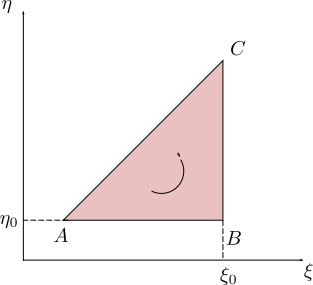
\includegraphics[width=0.2\textwidth]{figHyperRiman2.pdf}
\end{wrapfigure}
\begin{minipage}[t]{0.7\textwidth}
\[
	\oint\limits_{\partial D} \left(v \derp{w}{\eta}{} - w \derp{v}{\eta}{} \right) \, d\eta - \left(v \derp{w}{\xi}{} - w \derp{v}{\xi}{}\right)\, d\xi = 0\\
\]
\[
	\oint = \int\limits_A^B + \int\limits_B^C + \int\limits_C^A = 0
\]
\end{minipage}\\

\begin{multline*}
	\oint\limits_{\partial D}  \left(v \derp{w}{\eta}{} - w \derp{v}{\eta}{} \right) \, d\eta - \left(v \derp{w}{\xi}{} - w \derp{v}{\xi}{}\right)\, d\xi = \\ 
	= - \int\limits_A^B \left(v \derp{w}{\xi}{} - w \derp{v}{\xi}{} \right)\, d\xi + \int\limits_B^A \left(v \derp{w}{\eta}{} - w \derp{v}{\eta}{} \right)\, d\eta + \int\limits_C^A \left[\left(v \derp{w}{\eta}{} - w \derp{v}{\eta}{} \right)\, d\eta - \left(v \derp{w}{\xi}{} - w \derp{v}{\xi}{} \right)\, d\xi \right] = \\
	= - wv \Big|_A^B + 2 \int\limits_A^B w \derp{v}{\xi}{} d \xi + v w \Big|_B^C - 2 \int\limits_B^C w \derp{v}{\eta}{}\, d\eta + \int\limits_C^A [\ldots] = -2 w v\Big|_B + w v\Big|_A + w v\Big|_C + \int\limits_C^A [\ldots] = 0
\end{multline*}
\[
	w v\Big|_B = \frac{wv\Big|_A + w v\Big|_C}{2} + \frac{1}{2} \int\limits_C^A \left[ \left(v \derp{w}{\eta}{} - w \derp{v}{\eta}{} \right) - \left(v \derp{w}{\xi}{} - w \derp{v}{\xi}{} \right)\, d\xi\right]
\]
%($u_n$ -- производная по направлению нормали к кривой $S$), и выясним область, в которой решение определяется начальными условиями.


%Кривая $S$ задана уравнением
%\[
%	y = g(x)
%\]
%где $g(x)$ -- дифференциируемая функция. Наложим на кривую $S$ условие, чтобы всякая характеристика семейств $y - x = const$ и $y + x = const$ пересекала кривую $S$ не более одного раза (для этого нужно, чтобы $\abs{g'(x)} < 1$). 

%\begin{align*}
%	&v l[w] - w l^*[v] = v \left(\derps{v}{\xi}{\eta}+ \frac{1}{4} w\right) - w\left(\derps{v}{\xi}{\eta} + \frac{1}{4} v \right) = \frac{1}{2} \derp{}{\xi}{} \left(w \derp{w}{\eta}{} \right) - \frac{1}{2} \derp{}{\eta}{} \left(v \derp{v}{\xi}{} \right) \\
%	&v l[w] - w l^*[v] = \frac{1}{2} \frac{\partial}{\partial \xi}\left(v \der{w}{\eta}{} \right) - \frac{1}{2} \frac{\partial}{\partial \xi}\left(v \der{v}{\eta}{} \right) + \frac{1}{2} \frac{\partial}{\partial \eta}\left(v \der{w}{\eta}{} \right) - \frac{1}{2} \frac{\partial}{\partial \eta}\left(w \der{v}{\eta}{} \right)
%\end{align*}
%\[
%	\frac{1}{2} \frac{\partial}{\partial \xi}\left(v \der{w}{\eta}{} - w \der{v}{\eta}{} \right) + \frac{1}{2} \frac{\partial}{\partial \eta}\left( v \der{w}{\xi}{} - w \der{v}{\xi}{} \right) = 0
%\]
%Проинтегрируем это выражение
%\[
%	\iint\limits_D \frac{1}{2} \frac{\partial}{\partial \xi}\left(v \der{w}{\eta}{} - w \der{v}{\eta}{} \right) + \frac{1}{2} \frac{\partial}{\partial \eta}\left( v \der{w}{\xi}{} - w \der{v}{\xi}{} \right) d\xi d\eta = 0
%\]
%Применяем формулу Грина
%\[
%	\oint\limits_G \left(v \der{w}{\eta}{} - w \der{v}{\eta}{} \right) d\eta - \oint\limits_G \left(v \der{w}{\xi}{} - w \der{v}{\xi}{} \right) d\xi = 0
%\]
%\begin{multline*}
%	\oint = \int\limits_A^B + \int\limits_B^C+ \int\limits_C^A = \int\limits_A^B \left(v \der{w}{\eta}{} - w \der{v}{\eta}{} \right) d\eta - \int\limits_B^C \left(v \der{w}{\xi}{} - w \der{v}{\xi}{} \right) d\xi +\\{} + \oint\limits_G \left(v \der{w}{\eta}{} - w \der{v}{\eta}{} \right) d\eta -  \left(v \der{w}{\xi}{} - w \der{v}{\xi}{} \right) d\xi = 0
%\end{multline*}
%\[
%	- w v \Big|_A^B + \int\limits_A^B w \left(\der{v}{\xi}{} + \der{v}{\eta}{} \right) d \xi + v %w\Big|_B^C - \int\limits_B^C w \left(\der{v}{\eta}{} + \der{v}{\eta}{}\right) d \eta + \int\limits_C^A \ldots= 0
%\]
%%Потребуем чтобы выполнялись граничные условия:
%\begin{align*}
%	&AB: \der{v}{\xi}{} = 0\\
%	&BC: \der{v}{\eta}{} = 0\\
%\end{align*}
%\[
%	\frac{(wv)_A + (vw)_C}{2} + \frac{1}{2} \int\limits_C^A \left(v \der{w}{\eta}{} - w \der{v}{\eta}{} \right) d\eta -  \left(v \der{w}{\xi}{} - w \der{v}{\xi}{} \right) d\xi = (wv)_B
%\]

	
Найдём функцию Римана.
\[
	\derps{v}{\xi}{\eta} + \frac{1}{4} v = 0
\]
Будем искать $v$ в виде $v =\Phi(\lambda); \quad \lambda= \sqrt{(\xi - \xi_0)(\eta - \eta_0))}$\\
\begin{align*}
	&\derp{v}{\xi}{} =\Phi'(\lambda) \derp{\lambda}{\xi}{}  &\derps{v}{\xi}{\eta} = \derp{}{\eta}{} \left(f'(\lambda) \derp{\lambda}{\xi}{}\right) =\Phi'' \derp{\lambda}{\xi}{} \derp{\lambda}{\eta}{}  +\Phi' \derps{\lambda}{\xi}{\eta}
\end{align*}
\[
	\derps{\lambda}{\xi}{\eta} = \frac{(\xi - \xi_0)}{2 \sqrt{(\xi - 'xi_0)(\eta - \eta_0)}} = \frac{1}{2} \sqrt{\frac{\xi - \xi_0}{\eta -\eta_0}} \derp{\lambda}{\xi}{} = \frac{1}{2} \sqrt{\frac{\eta - \eta_0}{\xi - \xi_0}}
\]
\[
	\derps{\lambda}{\xi}{\eta} = \frac{1}{4 \sqrt{(\xi - 'xi_0)(\eta - \eta_0)}} = \frac{1}{4 \lambda}
\]
\begin{equation}
	\Phi'' + \frac{\Phi'}{\lambda} + \Phi = 0
	\label{equ:equRimanBessel}
\end{equation}
Уравнение \eqref{equ:equRimanBessel} является уравнением Бесселя нулевого порядка.
\[
	\Phi = J_0(\lambda) = \sum\limits_{k = 0}^{\infty} \frac{\lambda^{2k}}{2 k!!}, \quad \Phi(0) = 1
\] 
Итак, искомая функция Римана $v = J_0 (\lambda)$\\
на прямой $AB$
\[
	\lambda = 0 \Rightarrow \derp{v}{\xi}{} = J_0'(\lambda) \derp{\lambda}{\xi}{} \Big|_{\eta=\eta_0} = 0
\]
на прямой $BC$ 
\[
	\derp{v}{\eta}{} = J_0'(\lambda) \derp{\lambda}{\eta}{}\Big|_{\xi = \xi_0} = 0
\]
В точке $B$ $v(b) = 1 = v(A) = v(c)$. Так как $\xi = \eta \Rightarrow d\xi = d\eta$, тогда 
\[
	w(B) = \frac{w(A) + w(C)}{2} + \frac{1}{2} \int\limits_C^A \left[ v \left(\derp{w}{\eta}{} - \derp{w}{\xi}{} \right) - w \left(\derp{v}{\eta}{} - \derp{v}{\xi}{}\right)\right]\, d\xi
\]
Известно, что 
\[
	b\left(\derp{w}{\eta}{} - \derp{w}{\xi}{} \right) = - g\left(\frac{a}{b}\xi\right) - \frac{b_0}{a_0} f\left(\frac{a}{b} \xi\right)
\]
\begin{align*}
	&\derp{v}{\eta}{} = J_0'(\lambda) \frac{(\xi - \xi_0)}{\sqrt{(\xi - \xi_0)(\eta - \eta_0)}} & \derp{v}{\xi}{} = J'(\lambda) \frac{\eta - \eta_0}{\sqrt{(\eta - \eta_0)(\xi - \xi_0)}}
\end{align*}
\[
	\derp{v}{\eta}{} - \derp{v}{\xi}{} = J_0'(\lambda) \frac{(\eta_0 - \xi_0)}{\sqrt{(\eta - \eta_0) (\xi - \xi_0)}}
\]

В итоге получаем
\begin{multline}
	w (\xi_0, \eta_0) = \frac{f\left(\frac{a}{b} \eta_0 \right) + f\left(\frac{a}{b} \xi_0 \right)}{2} +{}\\
	+\frac{1}{2} \int\limits_{\xi_0}^{\eta_0} \left\{J_0(\lambda) \left(- \frac{1}{b}  \right) \left(g\left(\frac{a}{b}\xi\right) + \frac{b_0}{a_0} f\left(\frac{a}{b} \xi\right) \right) - f \left(\frac{a}{b} \xi \right) \frac{J'(\lambda)(\eta_0 - \xi_0)}{\sqrt{(\eta - \eta_0)(\xi - \xi_0)}} \right\} d\xi
\end{multline}
%\[
%	\xi  + \eta = 2 b t \quad t = \frac{\xi + \eta}{2 b} \quad x = \frac{(\xi +\eta)u}{2b}
%\]

%Найдём производные
%\[
%	\derps{v}{\xi}{\eta} = \frac{1}{4 \sqrt{(\xi - \xi_0)(\eta - \eta_0))}}
%\]
%\[
%	\der{v}{\xi}{} =\Phi'(\lambda) \der{\lambda}{\xi}{} 
%\]
%\[
%	\quad\Phi'' \frac{1}{4} +\Phi' \frac{1}{4 \sqrt{(\xi - \xi_0)(\eta - \eta_0))}} + \frac{1}{4} = 0
%\]

%Мы рассматривали похожее уравнение\\
%\[
%	y'' + \frac{1}{x}y' + y = 0
%\]
%функция Бесселя.
%\[
%\Phi = J_0(\lambda)
%\]
%\[
%	J_0(0) = 1
%\]

%В нашем случае искомая функция Римана - функция Бесселя. \\
%\[
%	v = J_0(\lambda)
%\]
%На прямой AB $\lambda = 0$. И мы получаем \\
%\[
%	AB: \der{v}{\xi}{} = J_0'(\lambda) \der{\lambda}{\xi}{}|_{\eta - \eta_0} = 0
%\]
%	
%Смотрим для точки B.\\
%\[
%	B: \xi = \xi_0 \eta = \eta_0 \rightarrow
%\]
%\begin{align*}
%	&\lambda = 0\\
%	&i_0(0) = 1\\
%	&v|_b J_0(0) = 1\\
%\end{align*}

%\includegraphics{graphic}

%\[
%	\derps{w}{\xi}{\eta} + \frac{1}{4} w = 0
%\]
%\[
%		\xi = \eta \quad w =\Phi(\frac{a}{b}\xi)
%\]
%\[
% b \left(\derp{w}{\xi}{} - \derp{w}{\eta}{}\right) = g\left(\frac{a}{b}\xi\right) + \frac{b_0}{a_0}\Phi\left(\frac{a}{b}\xi\right) 
%\]
%\begin{multline*}
%	w(\xi_0, \eta_0) = \frac{w_a + w_c}{2} + \frac{1}{2} \int\limits_c^a \left[\left(v\derp{w}{\eta}{} - w \derp{v}{\eta}{}\right)d\eta - \left(v\derp{w}{\xi}{} - w \derp{v}{\eta}{}\right)\, d\xi \right] = \\ = \frac{w_a - w_c}{2} + \frac{1}{2} \int\limits_c^a \left[v \left(\derp{w}{\eta}{} - \derp{w}{\xi}{}\right) - w \left(\derp{v}{\eta}{} - \derp{v}{\xi}{}\right)\right]d\xi
%\end{multline*}
%\[
%	v = J_0(\lambda): \quad \lambda = \sqrt{(\xi - \xi_0)(\eta - \eta_0)}
%\]
%\[
%	\xi = \frac{b}{a}(x + at)
%\]
%\[
%	\eta = \frac{b}{a}(x - at) \quad J_0(0) = 1
%\]
%\[
%	\derp{v}{\eta}{} = J_0'(\lambda) \frac{\xi - \xi_0}{\sqrt{(\xi - \xi_0)(\eta - \eta_0))}}
%\]
%\[
%	\derp{v}{\xi}{} = J'(\lambda) \frac{\eta - \eta_0}{\sqrt{(\xi - \xi_0)(\eta - \eta_0))}}
%\]
\end{example}

 \newpage 

\section{Уравнения параболического типа.}
	\subsection{Вывод уравнения теплопроводности}\label{que:2}
		Уравнения с частными производными 2-го порядка параболического типа часто встречаются при изучении процессов теплопроводности и диффузии.

\begin{figure}[h!]
    \centering
    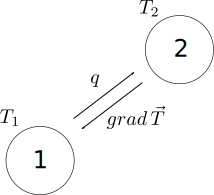
\includegraphics[scale=0.7]{figWarm.pdf}
	
	\label{fig:figWarm}
    \end{figure}
	При постоянных температурах $T_1$ и $T_2$ тепло перетекает от более нагретого участка к менее нагретому. Градиент направлен в сторону возрастания тепла.

\textbf{Закон Фурье}:
\[
	q = - k\, \mathrm{grad} T 
\]
Поток тепла пропорционален градиенту температуры.  $q$ - количество тепла, протекающего за единицу времени через единицу площади.  $q$ --- коэффициент теплопроводности материала.

\begin{wrapfigure}{r}{0.4\textwidth}
	\centering
	\includegraphics[width=0.4\textwidth]{figWarm2.pdf}
\end{wrapfigure}
Возьмём бесконечно малый объём. Рассмотрим грани куба. Перпендикулярно оси $x$ через грань II выохдит тепловой поток.  Найдём разность между тепловым потоком, вошедшим в I и вышедшим из II.

За время $dt$ в куб входит количество тепла $q_y\, dx dz dt$, а выходит $- q_y(y + dy)\, dx dz dt$.
\[
	q_y(y)\, dx dz dt = - q_y(y + dy)\, dx dz dt 
\]
Мы можем разложить функцию в ряд Тейлора, пользуясь малостью $dy$:
\[
	q_y(y)\, dx dz dt  - q_y(y + dy)\, dx dz dt  - \derp{q_y}{y}{} (y)\, dx dy dz
\]
Пренебрегая малыми 2-го порядка мы получили формулу тепла, которое осталось внутри куба.
\[
	\left(-\derp{}{x}{} q_x - \derp{}{y}{} q_y - \derp{}{z}{} q_z \right)\, dx dy dz  dt
\]
Количество тепла, которое нужно сообщить одному телу, чтобы повысить его температуру на $\Delta T$ равно
\[
	Q = c m \Delta T
\]
где $m= c \rho \,dx dy dz dT$.

Подставляем $Q$
\[
	c \rho \, dT dx dy dz = \left(-\derp{}{x}{} q_x - \derp{}{y}{} q_y - \derp{}{z}{} q_z \right)\, dx dy dz  dt.
\]
Приходим к следующей формуле
\[
	c \rho \derp{T}{t}{} = - \left(\derp{}{x}{}q_x + \derp{}{y}{} q_y + \derp{}{z}{} q_z \right)
\]

Из закона Фурье определим проекции $q_x, q_y, q_z$
\[
	\overrightarrow{\mathrm{grad}} T = \derp{T}{x}{} \vec i + \derp{T}{y}{} \vec j + \derp{T}{z}{} \vec k
\]
\[
	q = - k \overrightarrow{\mathrm{grad}} T
\]
\begin{align*}
	&q_x = - k_x \derp{T}{x}{} &q_y = - k_y \derp{T}{y}{} &q_z = - k_z \derp{T}{z}{}
\end{align*}


Наше тело изотропно, то есть зависит от времени
\[
	c \rho \derp{T}{t}{} = \derp{}{x}{} \left(k_x \derp{T}{x}{} \right) + \derp{}{y}{} \left(k_y \right) + \derp{}{z}{} \left(k_z \derp{T}{z}{} \right)
\]
\[
	\derp{T}{t}{} = \frac{k}{c \rho} \left( \derp{T}{x}{2} + \derp{T}{y}{2} + \derp{T}{z}{2} \right), \quad k_x = k_y = k_z = k = const
\]
\[
	\frac{k}{c \rho} = a^2
\]
где $a$ --- коэффициент температуропроводности, а $c$ --- коэффициент теплоёмкости.
Будем рассматривать уравнение в одномерном случае:
\begin{equation}
	\derp{T}{t}{} = a^2\derp{u}{x}{2}
	\label{equ:equWarm2}
\end{equation}
	Уравнение \eqref{equ:equWarm2} называется \textit{уравнением теплопроводности}.
 \newpage

	\subsection{Метод Фурье для уравнения теплопроводности}\label{que:16}
		\setcounter{equation}{0}
Однородная краевая задача для уравнения теплопроводности на отрезке:
\begin{equation}
	\derp{u}{t}{} = a^2 \derp{u}{x}{2} + f(x, t), \quad (0 < x <l, t > 0)
	\label{equ:HeatEqu}
\end{equation}
с начальным условием 
\begin{equation}
	u(x, 0) = \varphi(x), \quad (0 \leqslant x \leqslant l)
	\label{equ:HeatStartCond}
\end{equation}
и граничным условиям 
\begin{equation}
	\left.
	\begin{aligned}
		u(0, t) &= \mu_1 (t),\\
		u(l, t) &= \mu_2 (t)
	\end{aligned}
	\right\} \quad
	(t \geqslant 0).
	\label{equ:HeatBorderCond}
\end{equation}

Изучение общей первой краевой задачи начнём с решения следующей простейшей задачи $I$:\\
	\textit{найти непрерывное в замкнутой области $(0 \leqslant x \leqslant l, 0 \leqslant t \leqslant T)$ решение однородного уравнения}

\begin{equation}
	\derp{u}{t}{} = a^2 \derp{u}{x}{2}, \qquad 0 < x < l,\quad  0 < t \leqslant T,
	\label{equ:equHeatEquSimp}
\end{equation}
\textit{удовлетворяющее начальному условию}
\begin{equation}
	u(x, 0) = \varphi (x), \quad 0 \leqslant x \leqslant l
	\label{equ:equHeatEquSimpStartCond}
\end{equation}
\textit{и однородным граничным условиям}
\begin{equation}
	u(0, t) = 0, \quad u(l, t) = 0, \quad 0 \leqslant t \leqslant T.
	\label{equ:equHeatEquSimpBorderCond}
\end{equation}

Для решения этой задачи рассмотрим, как принято в методе разделения переменных, сначала основную вспомогательную задачу:\\
\textit{найти решение уравнения}
\[
	u_t = a^2 u_{xx},
\]
не равное тождественно нулю, удовлетворяющее однородным граничным условиям
\begin{equation}
	u(0, t) = 0, \quad u(l, t) = 0 
	\label{equ:equHeatEqu2Border}
\end{equation}
\textit{и представимое в виде}
\begin{equation}
	u(x, t) = X(x) T(t),
	\label{equ:equHeatEquFourierView}
\end{equation}
\textit{где $X(x)$ -- функция только переменного $x$, $T(t)$ -- функция только переменного $t$.}

Подставляя предполагаемую форму решения \eqref{equ:equHeatEquFourierView} в уравнение \eqref{equ:equHeatEquSimp}  и производя деление обеих частей равенства на $a^2 X T$, получим: 
\begin{equation}
	\frac{1}{a^2} \frac{T'}{T} = \frac{X''}{X} = - \lambda
	\label{equ:equHeatEquFourierView}
\end{equation}
где $\lambda = const$, так как левая часть равенства зависит только от $t$, а правая -- только от $x$.
Отсюда следует, что
\begin{gather}
	X'' + \lambda X = 0
	\label{equ:equHeat1}\\
	T' + a^2 \lambda T = 0
	\label{equ:equHeat2}
\end{gather}

Граничные условия \eqref{equ:equHeatEqu2Border} дают:\\
\begin{equation}
	X(0) = 0, \quad X(l) = 0.
	\label{equ:equHeat3}
\end{equation}

Таким образом, для определения функции $X(x)$ мы получили задачу о собственных значениях (задачу Штурма --- Лиувилля)
\begin{equation}
	X'' + \lambda X =0, \quad X(0) = 0, X(l) = 0,
	\label{equ:equHeatShturm}
\end{equation}
исследованную при решении уравнения колебаний. При этом было показано, что только для значений параметра $\lambda$, равных 
\[
	\lambda_n = \left(\frac{\pi n}{l} \right)^2 \quad (n = 1, 2, 3, \ldots),
\]
существуют нетривиальные решения уравнения \eqref{equ:equHeatEquFourierView}, равные
\begin{equation}
	X_n(x) = \sin \frac{\pi n}{l} x.
	\label{equ:equHeat4}
\end{equation}
Этим значениям $\lambda_n$ соответствуют решения уравния \eqref{equ:equHeat2}
\[
	T_n(t) = C_n e^{-a^2 \lambda_n t},
\]
где $C_n$ -- не определённые коэффициенты.

Возвращаясь к основной вспомогательной задаче, видим, что функции
\[
	u_n(x, t) = X_n(x) T_n(t) = C_n e^{-a^2 \lambda_n t} \sin \frac{\pi n}{l} x,
\]
являются частными решениями уравнения \eqref{equ:equHeatEquSimp}, удовлетворяющими нулевым граничным условиям. \\


Обратимся теперь к решению задачи (I). Составим формально ряд
\begin{equation}
	u(x,  t) = \sum\limits_{n = 1}^{\infty} C_n e^{-a^2 \lambda_n t} \sin \frac{\pi n}{l} x.
	\label{equ:equHeatRow1}
\end{equation}
Функция $u(x, t)$ удовлетворяет граничным условиям, так как им удовлетворяют все члены ряда. Требуя выполнения начальных условий, получаем:
\begin{equation}
	\varphi(x) = u(x, 0) = \sum\limits_{n = 1}^{\infty} C_n \sin \frac{\pi n}{l} x,
	\label{equ:equHeatRow2}
\end{equation}
т.е. $C_n$ являются коэффициентами Фурье функции $\varphi(x)$ при разложении её в ряд по синусам на интервале $(0, l)$:
\begin{equation}
	C_n = \varphi_n = \frac{2}{l} \int\limits_0^l \varphi(\xi) \sin \frac{\pi n}{l} \xi \, d\xi.
	\label{equ:equHeatFRow3}
\end{equation}
Рассмотрим теперь ряд \eqref{equ:equHeatRow1} с коэффициентам $C_n$, определяемыми по формуле \eqref{equ:equHeatFRow3}, и покажем, что этот ряд удовлетворяет всем условиям задачи (I). Для этого надо доказать, что функция $u(x, t)$, определяемая рядом \eqref{equ:equHeatRow1}, дифференциируема, удовлетворяет уравнению в области $0 < x < l, \quad t > 0$ и непрерывна в точках границы этой области (при $t = 0, x = 0, x = l$).

Так как уравнение \eqref{equ:equHeatEquSimp} линейно, то в силу принципа суперпозиции ряд, составленный из частных решений, также будет решением, если он сходится и его можно дифференциировать почленно дважды по $x$ м один раз по $t$. Покажем, что при $t \geqslant t > 0$ ($t$ -- любое вспомогательное число) ряды производных
\[
	\sum\limits_{n = 1}^{\infty} \derp{u_n}{t}{} \quad \mbox{и} \quad \sum\limits_{n = 1}^{\infty} \derp{u_n}{x}{2}
\] 
сходится равномерно. В самом деле,
\[
	\abs{\derp{u_n}{t}{}} = \abs{- C_n \left(\frac{\pi}{l}\right)^2 a^2 n^2 e^{-\left(\frac{\pi n}{l}\right)^2 a^2 t} \sin \frac{\pi n}{l} x} < \abs{C_n} \left(\frac{\pi}{l}\right)^2 \cdot a^2 n^2 e^{-\left(\frac{\pi n}{l}\right)^2 a^2 t}
\]
В дальнейшем будут сформулированы дополнительные требования, которым должна удовлетворять фукнция $\varphi(x)$. Предположим сначала, что $\varphi(x)$ ограничена, $\abs{\varphi(x)} < M$; тогда
\[
	\abs{C_n} = \abs{\frac{2}{l}} \abs{\int_0^l \varphi(\xi) \sin \frac{\pi n}{l}\xi\, d\xi} < 2M
\]

откуда следует, что 
\[
	\abs{\derp{u_n}{t}{}} < 2 M \left(\frac{\pi}{l}\right)^2 a^2 n^2 e^{-\left(\frac{\pi n}{l}\right)^2 a^2 \bar t} \quad \mbox{для}\quad t \geqslant \bar t
\]
и аналогично
\[
	\abs{\derp{u_n}{x}{2}} < 2 M \left(\frac{\pi}{l}\right)^2 a^2 n^2 e^{-\left(\frac{\pi n}{l}\right)^2 a^2 \bar t} \quad \mbox{для}\quad t \geqslant \bar t.
\]

Вообще
\[
	\abs{\frac{\partial^{k+1} u_n}{\partial t^k\,\partial x^l}} < 2 M \left(\frac{\pi}{l}\right)^{2k + l} \cdot n^{2k + l} \cdot a^{2k} \cdot  e^{-\left(\frac{\pi n}{l}\right)^2 a^2 \bar t}\quad \mbox{для}\quad t \geqslant \bar t.
\]

Исследуем сходимость мажорантного ряда $\sum\limits_{n = 1}^{\infty} \alpha_n$, где 
\begin{equation}
	\alpha_n = N n^q e^{-\left(\frac{\pi n}{l}\right)^2 a^2 \bar t}.
	\label{equ:equHeatFR1}
\end{equation}

По \href{http://clck.ru/W/E9fB}{признаку Далабмера} ряд сходится, так как
\[
	\lim\limits_{n \to \infty} \abs{\frac{\alpha_{n + 1}}{\alpha_n}} = \lim\limits_{n \to \infty} \frac{(n + 1)^q}{n^q} \frac{e^{-\left(\frac{\pi}{l}\right)^2 a^2 (n^2 + 2 n + 1) \bar t}}{e^{-\left(\frac{\pi}{l}\right)^2 a^2 n^2 \bar t}} = \lim\limits_{n \to \infty} \left( 1 + \frac{1}{n}\right)^q e^{-\left(\frac{\pi}{l}\right)^2 a^2 (2n + 1) \bar t} = 0.
\]
Отсюда вытекает возможность почленного дифференциирования ряда \eqref{equ:equHeatRow1} любое число раз в области $t \geqslant \bar t > 0$. Далее, пользуясь принципом суперпозиции, заключаем, что функция определённая этим рядом, удовлетворяет уравнению \eqref{equ:equHeatEquSimp}. В силу произвольности  $\bar t$ это имеет место для всех $t > 0$. Тем самым доказано, что при $t > 0$ ряд \eqref{equ:equHeatRow1} представляет функцию, дифференциируемую нужное число раз и удовлетворяющую уравнению \eqref{equ:equHeatEquSimp}.

\textit{Если функция $\varphi(x)$ непрерывная, имеет кусочно-непрерывную производную и удовлетворяет условиям $\varphi(0)=0$ и $\varphi(l) = 0$, от ряд \eqref{equ:equHeatRow1}}
\[
	u(x,  t) = \sum\limits_{n = 1}^{\infty} C_n e^{-a^2 \lambda_n t} \sin \frac{\pi n}{l} x.
\]
\textit{определяет \href{http://5z8.info/enriched-uranium-supply_b4w8xn_illegal-guns-for-sale}{непрерывную функцию} при $t \geqslant 0$.}

Действительно, из неравенства 
\[
	\abs{u_n(x, t)} < \abs{C_n} \quad (\mbox{при} t \geqslant 0, 0 \leqslant x \leqslant l)
\]
сразу же следует равномерная сходимость ряда \eqref{equ:equHeatRow1} при $t \geqslant 0$, $0 \leqslant x \leqslant l$, что и доказывает справедливость сделанного выше утверждения, если учесть, что для непрерывной и кусочно-гладкой функции $\varphi(x)$ ряд из модулей коэффициентов Фурье сходится, если $\varphi(0) = \varphi(l) = 0$.\\

Итак, задача нахождения решения прямой краевой задачи для однородного уравнения с нулевыми граничными условиями и непрерывным, кусочно-гладким начальным условием решена полностью. \newpage

	\subsection{Задача Коши для бесконечного стержня}\label{que:17}
		Рассмотрим задачу Коши:
\[
	\derp{u}{t}{} = a^2 \derp{u}{x}{2}, \quad t > 0\\
\]
Начальное условие:
\[
	u(x, 0) = f(x)
\]
\[
	t a^2 = T \Rightarrow \derp{u}{T}{} = \derp{u}{x}{2}
\]
Будем искать ограниченное нетривиальное решение уравнения методом разделения переменных, представимое в виде
\[
	u = X(x) Y(t) 
\]
Подставляя это выражение в исходное уравнение, получаем:
\[
	\quad \frac{X''}{X} = \frac{Y'}{Y} = - \lambda^2,
\]
где $\lambda^2$ -- параметр разделения.\\
Частные решения находятся в таком виде
\begin{align*}
	&X(x) = \alpha (\lambda) \sin \lambda x + \beta (\lambda) \cos \lambda x\\
	&Y(t) = e^{- \lambda^2 t}
\end{align*}
Общее решение
\[u(x, t) = (\alpha (\lambda) \sin \lambda x + \beta(\lambda) \cos \lambda x) e^{-\lambda^2 t}\] 
Запишем интегральный вид уравнения
\[u(x, t) = \int\limits_{-\infty}^{+ \infty} (\alpha (\lambda) \sin \lambda x + \beta (\lambda) \cos \lambda x) e^{-\lambda^2 t} \,  d \lambda\]
Из начальных условий найдём неизвестные
\[u(x, 0) = \int\limits_{-\infty}^{+ \infty} (\alpha (\lambda) \sin \lambda x + \beta (\lambda) \cos \lambda x) d\lambda = f(x)\]
\[\alpha (\lambda) = \frac{1}{2 \pi} \int\limits_{- \infty}^{+ \infty} f (\xi) \sin \lambda \xi \, d \xi\]
\[\beta(\lambda) = \frac{1}{2 \pi} \int\limits_{- \infty}^{+ \infty} f (\xi) \cos \lambda \xi \, d \xi\]
Подставляя в уравнение и меняя порядок интегрирования получим
\[u(x,t) = \frac{1}{2 \pi} \iint\limits_{R^2} f(\xi) (\sin \lambda x \sin \lambda \xi + \cos \lambda x \cos \lambda \xi) e^{- \lambda^2 t} \, d \lambda d \xi \]
\[u(x, t) = \frac{1}{2 \pi} \iint\limits_{R^2} f(\xi) \cos \lambda (x - \xi) e^{- \lambda^2 t} \, d \lambda  d \xi\]
Произведём замену переменных
\[
	\int\limits_{- \infty}^{ + \infty} \cos \lambda (x - \xi) e^{- \lambda^2 t} \, d \lambda = \left[ 
		\begin{tabular}{l}
			$\lambda \sqrt{t} = \sigma$\\ 
			$\lambda(x - \xi) = \sigma \omega$ 
		\end{tabular} \right] 
	= \int\limits_{- \infty}^{ + \infty} \cos \sigma \omega e^{- \sigma^2} \frac{d \sigma}{\sqrt{t}}
\]
Возьмём этот интаграл. Для удобства обозначим его как
\[I(\omega) = \int\limits_{- \infty}^{ + \infty} \cos \omega \sigma e^{- \sigma^2} \, d \sigma\]
Найдём производную по $\omega$
\[\der{I}{\omega}{} = - \int\limits_{- \infty}^{ + \infty}\sigma \sin \sigma \omega e^{- \sigma^2} d \sigma - \frac{\omega}{2} \int\limits_{- \infty}^{ + \infty} \cos \sigma \omega e^{-\sigma^2} d \sigma\]
\[I(\omega) = \sqrt{\pi} e^{- \frac{(x - \xi)^2}{4}} = \sqrt{\pi} e^{-\frac{\omega^2}{4}}\]
В итоге получаем
\[\int\limits_{- \infty}^{ + \infty} \cos (x - \xi) e^{- \lambda^2 t} \, d \lambda = \sqrt{\frac{\pi}{t}}  e^{- \frac{(x - \xi)^2}{4 t}}\]
Подставим в общее решение
\[u(x, t) = \sqrt{\frac{\pi}{t}} \int\limits_{- \infty}^{ + \infty} f(\xi) e^{- \frac{(x - \xi)^2}{4 t}} \, d \xi \cdot \frac{1}{2 \pi}\]
Окончательное решение:\\
\[u(x, t) = \frac{1}{2 a \sqrt{\pi t}} \int\limits_{- \infty}^{ + \infty} f(\xi)  e^{- \frac{(x - \xi)^2}{4 a^2 t}} \, d \xi\]\\
Проверим, что это действительно решение:\\
\[t=0 \quad \lim\limits_{t \downarrow 0} u(x, t) = \int\limits_{- \infty}^{ + \infty} f(\xi) \delta (\xi - x) \, d \xi = f(x)\]
\[G(x, \xi, t) = \frac{e^{- \frac{(x - \xi)^2}{4 a^2 t}}}{2 a \sqrt{\pi t}}\]
Продифференциируем функцию $G(x, \xi, t)$
\begin{align*}
	&\derp{G}{t}{} = \left( \frac{(x - \xi)^2}{2\cdot 4 a^3 t^2 \sqrt{t}} -\frac{1}{4 a t \sqrt{\pi t}}  \right) e^{- \frac{(x - \xi)^2}{4 a^2 t}}\\
	&\derp{G}{x}{} = - \frac{\cancel 2 (x - \xi)^2}{4 a^2 t} \cdot \frac{1}{\cancel 2 a \sqrt{\pi t}} e^{- \frac{(x - \xi)^2}{4 a^2 t}}\\
	&\derp{G}{x}{2} = \left(\frac{2 (x - \xi)^2}{16 a^5 \sqrt{\pi t} t^2} - \frac{1}{4 a^3 t \sqrt{\pi t}} \right) e^{- \frac{(x - \xi)^2}{4 a^2 t}}
\end{align*}
Функция удовлетворяет уравнению теплопроводности по переменным $(x, t)$.

Итак, мы пришли к интегральному представлению искомого решения
\[
	u(x, t) = \int\limits_{- \infty}^{ + \infty} f(\xi)G(\xi, x, t) \, d \xi ,
\]
где
\begin{equation}
	G(x, \xi, t) = \frac{1}{2 a \sqrt{\pi t}} e^{- \frac{(x - \xi)^2}{4 a^2 t}}
	\label{equ:koshiInftyG}
\end{equation}
			Функцию $G(x, \xi, t)$, определяемую формулой \eqref{equ:koshiInftyG}, часто называют фундаментальным решением уравнения теплопроводности. \newpage		

	\subsection{Автомодельные решения задачи теплопроводности.}
		Некоторые задачи  представляют в виде функции от комбинации переменных $x$ и $t$.\\
	Рассмотрим пример:
		пусть  $z = \frac{x}{2 \sqrt{t}}$, задача теплопроводности имеет вид:
		\[\derp{u}{t}{} = \derp{u}{x}{2}\]
		Начальные условия:
		\[u(x, t) = u_0 f(z)\]
		\begin{alignat*}{2}			
			&u = u_0, &\quad x &\geqslant 0,\\
			&u = 0, &\quad x &< 0
		\end{alignat*}
		Считаем частные производные
		\[\derp{u}{t}{} = u_0 \der{f}{z}{} \derp{z}{t}{} = - \frac{x}{4 t \sqrt{t}} u_0 \der{f}{z}{}\]
		\[\derp{u}{x}{} = u_0 \der{f}{z}{} \frac{1}{2 \sqrt{t}} \quad \derp{u}{x}{2} = u_0 \der{f}{z}{2} \cdot \frac{1}{4 t}\]
		Подставляем в уравнение теплопроводности
		\[\cancel{- u_0} \frac{x}{\cancel{4t} \sqrt{t}} \der{f}{z}{} = \cancel{u_0} \frac{1}{\cancel{4 t}} \der{f}{t}{2}\]
		\[-2 z \der{f}{z}{} = \der{f}{z}{2}\]
		Получили дифференциальное уравнение 2-го порядка
		\[\der{f}{z}{2} + 2 z \der{f}{z}{} = 0\]
		Порядок уравнения можно понизить до первого следующей заменой:
		\[\der{f}{z}{} = \varphi \Rightarrow \der{\varphi}{z}{} = - 2z \varphi\]
		Полученное уравнение легко интегрируется 
		\[\ln \varphi = C - z^2 \Rightarrow \varphi = C e^{-z^2}\]
		\[f(z) = C \int\limits_0^z e^{-\xi^2} d \xi\]
		\[\lim_{t \to 0} u(x, t) = u_0 \Rightarrow \lim_{t \to 0} f(z) = 1 \Rightarrow C = \frac{2}{\sqrt{\pi}}\]
		Окончательно получаем:
		\[u(x, t) =  \frac{2 u_0}{\sqrt{\pi}} \int\limits_0^{- \frac{x}{2 \sqrt{t}}} e^{- \xi^2} d\xi\]	\newpage

	\subsection{Задача теплопроводности в цилиндрической системе координат}
		\[
	\left.\begin{aligned}
		\derp{u}{t}{} &= \derp{u}{r}{2} +\frac{1}{r} \derp{u}{r}{}\\
		u(R, t) &= f(t)= 0\\
		u(r, 0) &= \varphi(p)	
	\end{aligned}\right\}
\]
\begin{wrapfigure}{r}{0.5\textwidth} 
	\centering
	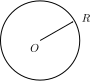
\includegraphics{figWarm1.pdf}		
\end{wrapfigure}
Будем искать решение в виде функции 
\[
	u = X(p)\cdot Y(t)
\]
Подставляем в уравнение
\[ 
	X(p)Y'(t) = Y(t) X''(p) +\frac{1}{p} Y(t) X'(p)
\]
Получаем следующее соотношение
\[
	\frac{Y'(t)}{Y(t)} = \frac{X''(p) + \frac{1}{p} X'(p)}{X(p)} = - k^2
\]
Для $X$ получаем дифференциальное уравнение 2-го порядка
\[
	X'' + \frac{1}{p} X' +k^2 X = 0
\]
Сделаем замену $\xi = k p$
\[
	  \der{X}{\xi}{2} + \frac{1}{\xi} \der{X}{\xi}{} + X = 0
\]
Будем искать решение в виде 
\[
	X(\xi) = \sum\limits_{k = 0}^{\infty} a_k \xi^k
\]
Находим первые две производные
\begin{align*}
	&X'(\xi)= \sum\limits_{k = 1}^{\infty} a_k k \xi^{k - 1}\\
	&X''(\xi) =  \sum\limits_{k = 2}^{\infty} a_k (k - 1) k \xi^{k - 2}
\end{align*}
и подставляем в полученное уравнение 
\[
	a_0 + a_1 \xi + a_1 \frac{1}{\xi} + \sum\limits_{k = 2}^{\infty} (a_k (k - 1) k \xi^{k - 2} + a_k k \xi^{k - 2} + a_k \xi^k) = 0 
\]
Приравнивая коэффициенты при соответствующих степенях $\xi$, находим $a_i$
\[
	\frac{1}{\xi} a_1 = 0 \quad \xi^0: a_0 + 4 a_2 = 0
\]

\[
	\xi^1 a_1 + 3 a_3 + 6 a_3 = 0 \Rightarrow  a_{2k + 1} = 0 \quad k \in N \cup {0}
\]
Получаем
\[
	X(p) = \sum (-1)^n \frac{\xi^{2n}}{2^{2n} (n!)^2}
\]~--функция Бесселя нулевого порядка.\\

Исследуем ряд на сходимость:\\
Достаточно показать, что n-ый член (при $n \rightarrow \infty$) стремится к 0.\\
	\[X(p) = I_0 (k p) = \sum (-1)^n \frac{(k p)^2n}{2^{2n} (n!)^2}\]

В итоге получаем
\[u_n(p, t) = c_n e^{- k_n^2 t} J_0 (k_n p)\]
Решение исходной задачи будет представляться в таком виде
\[u(p, t) = \sum\limits_{n = 0}^{\infty} u_n (p, t) = \sum\limits_{n = 0}^{\infty} C_n e^{- k_n^2 t} J_0(k_n p)\]
Определим $k_n$: $u(R, 0) = 0 \Rightarrow J_0(k_n R) = 0$\\
Уравнение решается и имеет счётное количество корней - $k_n$.

\[
	t=0 \quad u(\rho, 0) = \varphi(\rho ) = \sum\limits_{n =0 }^{\infty} C_n J_0 (k_n \rho) e^0
\]

Для функции Бесселя:\\ 
	\[\int\limits_0^R J_0 (k_n p) I_0(k_m p) p dp = \begin{cases} \frac{1}{2} {J_0'}^2 (k_n R) & k=m \\ 0 & k \neq m \end{cases}\]

Это свойство можно использовать для нахождения коэффициентов $C_n$ следующим образом
\[
	\int\limits_0^R\rho\varphi(\rho) J_0(k_N \rho) d\rho = C_n \int_0^R \rho J_0^2 (k_n \rho) d \rho
\]
\[
	C_n =\frac{\int\limits_0^R \rho \varphi(\rho) J_0 (k_n \rho) d \rho}{\int\limits_0^R \rho J_0^2 (k_n\rho) d\rho}
	\] \newpage

\section{Уравнения эллиптического типа.}
	\subsection{Вывод уравнения}
		При исследовании стационарных процессов различной физической природы (колебания, теплопроводность, диффузия, и др.) обычно приходят к уравнениям эллиптического типа. Наиболее распространённым уравнением этого типа является \textit{уравнение Лапласа}
\[
	\Delta u = 0
\]

Функция $u$ называется \textit{гармонической } в области $\Omega$, если она непрерывна в этой области вместе со своими производными до 2-го порядка и удовлетворяет уравнению Лапласа.\\ 


Предcтавления в различных системах координат
\begin{flalign*}
\begin{tabular}{l l}
	\textbf{В декартовой} &$\displaystyle\Delta u = \derp{u}{x}{2} + \derp{u}{y}{2} + \derp{u}{z}{2}$\\[10pt]
	\textbf{В цилиндрической} &$\displaystyle\Delta u = \derp{u}{r}{2} + \frac{1}{r} \derp{u}{r}{} \frac{1}{r} \derp{u}{\theta}{2} + \derp{u}{z}{2}$ \\[10pt]
	\textbf{В сферической} &$\displaystyle\Delta u = \derp{u}{r}{2} + \frac{2}{r} \derp{u}{r}{} + \frac{1}{r^2 \sin \theta} \derp{}{\theta}{} \left(\sin \theta \derp{u}{\theta}{} \right) + \frac{1}{r^2 \sin^2 \theta} \derp{u}{\varphi}{2}$\\
\end{tabular}
\end{flalign*}
Рассмотрим некоторый объём $\Omega$, ограниченный поверхностью $S$. 
\begin{figure}[h!]
	\centering
	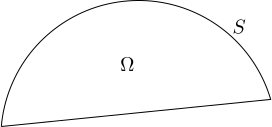
\includegraphics{figElliptic1.pdf}
	\label{fig:elliptic1}
\end{figure}\\
Задача о стационарном распределении температуры $u(x, y, z)$ внутри тела $\Omega$ формулируется следующим образом:\\

\textit{Найти функцию $u(x, y, z)$, удовлетворяющую внутри $\Omega$ уравнению}
\[
	\Delta u = - f(x, y, z)
\]
\textit{и граничному условию, которое может быть взято в одном из следующих видов:}
\begin{flalign*}
	\text{\Rmnum{1}. }&\quad u_g = f(x, y, z) &\mbox{первая краевая задача}\\
	\text{\Rmnum{2}. }&\quad \derp{u}{n}{}  = g (x, y, z)&\mbox{вторая краевая задача}\\
	\text{\Rmnum{3}. }&\quad  \derp{u}{n}{} + \alpha u = h(x, y, z ) &\mbox{третья краевая задача}
\end{flalign*}
\textit{где $f, g,  h$ -- заданные функции, $\derp{u}{n}{}$ --  производная по внешней нормали к поверхности $S$.}\\

Первую краевую задачу называют \textit{задачей Дирихле}, вторую \textit{задачей Неймана}. Третья задача  -- задача \textit{смешанная}. 


%\[
%	\iint\limits_S A_n dS \iiint\limits_{\omega} du A d \omega
%\]
%
%
%\[
%	\bar A = u grad v - v grad u
%\]
%\[
%	A_n =\bar A \cdot \bar n
%\]
%\[
%	A_n = u \bar grad v \bar n - v \bar grad u \cdot \bar n = u \der{v}{n}{} - v \der{u}{n}{}
%\]
 \newpage

	\subsection{Метод Фурье в задачах эллиптического типа}
		Решение краевых задач для уравнений Лапласа может быть найдено методом разделения переменных в случае некоторых простейших областей (круг, прямоугольник, шар и цилиндр и др.). Получающиеся при этом задачи на собственные значения (задачи Штурма--Лиувилля) приводят к различным классам специальных функций. Рассмотрим задачу Дирихле, при решении которой используются только тригонометрические функции. 









	

 

		\subsubsection{Первая краевая задача для круга}
			\[
	\Delta u = 0 \quad \mbox{ \textit{внутри круга}}
\]
Граничное условие
\[
	u\big|_{\Gamma} = f (\theta)
\]
$\Gamma$ -- окружность радиуса $R$
\[
	u|_{r = k} = f (\theta)
\]
тогда в полярной системе координат 
\[
	\Delta u = \derp{u}{r}{2} + \frac{1}{r} \derp{u}{r}{} + \frac{1}{r^2} \derp{u}{\theta}{2} = 0
\]
\\
\[
	u = F(r) \cdot G (\theta)
\]
\[
	\left. F'' G + \frac{1}{r} F' G + \frac{1}{r^2} F G'' = 0 \quad \right| \frac{r^2}{F G}
\]
\\
\[
	\frac{r^2 F'' + r F'}{F} = - \frac{G''}{G} = \lambda
\]
Получаем уравнения вида
\[
	G''(\theta) = - \lambda G(\theta) 
\]
\[
	r^2 F''(r) + r F'(r) = \lambda F(r)
\]

\[
	\lambda > 0\quad \lambda = \gamma^2 > 0 \quad \gamma = n
\]
\[
	r^2 F''(r) + r F'(r) - n^2 F(r) = 0
\]
Решения
\[
	G = A \cos \gamma \theta + B \sin \gamma \theta
\]
Функцию $F$ будем искать в виде $R(r) = r^\mu$. Подставляя в уравнение и сокращая на $r^\mu$, найдём 
\[
	n^2 = \mu^2 \quad \mbox{или} \quad  \mu = \pm n (n > 0).
\]
Следовательно
\[
	F = C_1 r^n + C_2 r^{-n}
\]

Для решения внутренней задачи надо положить $R = C_1 r^n\: (\mu = n)$, так как, если $C_2 \neq 0$, то функция $u = F(r) G(\theta)$ обращается в бесконечность при $r = 0$ и не является гармонической функцией вокруг круга. Для решения внешней задачи, наоборот, надо брать $R = C_2 r^{-n}\: (\mu = - n)$, так как решение внешней задачи должно быть ограничено  в бесконечности.


Так как $G$ должна иметь период $2 \pi$, то $\gamma = n$.
\[
	G = A \cos n \theta + B \sin n \theta, \quad  n \in \mathbb{N} 
\]
Таким образом частное решение для $r \leqslant R$ имеет вид
\[
	u_m = (C_1 A \cos n \theta + C_1 B \sin n \theta) r^n
\]
Сумма решения
\[
	u(r, \theta) =  \sum\limits_{n = 1}^{\infty} (C_{1n} \cos n \theta + C_{2n} \sin n \theta) r^n
\]
Найдём коэффициенты используя граничное условие
\begin{equation}
	u(\theta, R) =  C_{10} + \sum\limits_{n = 1}^{\infty} (C_{1n} \cos n \theta + C_{2n} \sin n \theta) R^n = f(\theta) 
	\label{equ:equBorder}
\end{equation}
Возьмём разложение $f(\theta)$ в ряд Фурье 
\begin{equation}
	f(\theta) = \frac{\alpha_0}{2} + \sum\limits_{n = 1}^{\infty} (\alpha_n \cos n \theta + \beta_n \sin n \theta)
	\label{equ:equFourierF}
\end{equation}
где 
\begin{align*}
	\alpha_0 &= \frac{1}{\pi} \int\limits_{-\pi}^\pi f(\psi)\, d \psi\\
	\alpha_n &=  \frac{1}{\pi} \int\limits_{-\pi}^\pi f(\psi) \cos n \psi\, d \psi \quad (n = 1, 2, \ldots)\\
	\beta_n &=  \frac{1}{\pi} \int\limits_{-\pi}^\pi f(\psi) \sin n \psi\, d \psi \quad (n = 1, 2, \ldots)
\end{align*}
Сравнивая \eqref{equ:equBorder} и \eqref{equ:equFourierF}, получаем 
\begin{align*}
	&C_{10} = \frac{\alpha_0}{2}, \quad C_{1n} = \frac{\alpha_n}{R^n}, \quad C_{2n} = \frac{\beta_n}{R^n}
\end{align*}

Таким образом, мы получили формальное решение первой внутренней задачи для круга в виде ряда
\begin{equation}
	u(\theta, r) =  \frac{\alpha_0}{2} + \sum\limits_{n = 1}^{\infty} (\alpha_n \cos n \theta + \beta_n \sin n \theta) \left(\frac{r}{R} \right)^n
	\label{equ:equSolveDirihletProblemRow}
\end{equation}

		\subsubsection{Интеграл Пуассона}
			С помощью преобразований \eqref{equ:equSolveDirihletProblemRow} получим решение в виде \textit{интеграла Пуассона}.

Подставляя выражения для кожффициентов Фурье в формулу \eqref{equ:equSolveDirihletProblemRow} и меняя порядок суммирования и интегрирования, будем иметь:
\begin{multline}
	u(\theta, r) = \frac{1}{\pi} \int\limits_{-\pi}^{\pi} f(\psi) \left\{ \frac{1}{2} + \sum\limits_{n = 1}^{\infty} \left(\frac{r}{R} \right)^n (\cos n \psi \cos n \theta + \sin n \psi \sin n \theta) \right\} \, d \psi = \\
	=  \frac{1}{\pi} \int\limits_{-\pi}^{\pi} f(\psi) \left\{ \frac{1}{2} + \sum\limits_{n = 1}^{\infty} \left(\frac{r}{R} \right)^n \cos n(\theta - \psi) \right\} \, d \psi 
	\label{equ:equPoisson1}
\end{multline}

Произведём следующие тождественные преобразования:
\begin{align*}
	\frac{1}{2} + \sum\limits_{n = 1}^{\infty} t^n \cos n (\theta - \psi) &= \frac{1}{2} + \frac{1}{2} \sum\limits_{n = 1}^{\infty} t^n \left[e^{in(\theta - \psi)} + e^{-in(\theta - \psi)}\right] = \\
	&= \frac{1}{2}\left\{1 + \sum\limits_{n = 1}^{\infty} [\left(t e^{i(\theta - \psi)}\right)^n + \left(t e^{-i(\theta - \psi)}\right)^n] \right\} =\\
	&= \frac{1}{2} \left[ 1 + \frac{t e^{i(\theta - \psi)}}{1 - t e^{i(\theta - \psi)}}  + \frac{t e^{-i(\theta - \psi)}}{1 - t e^{-i(\theta - \psi)}}\right] = \\
	&= \frac{1}{2} \frac{1 - t^2}{1 - 2t \cos(\theta - \psi) + t^2} &\left(t = \frac{r}{R} < 1 \right).
\end{align*}
Подставляя полученные результаты в равенство \eqref{equ:equPoisson1}, получаем:
\begin{equation}
	u (\theta, r) = \frac{1}{2 \pi} \int\limits_{- \pi}^{\pi} f(\psi) \frac{R^2 - r^2}{r^2 - 2  r R \cos (\theta - \psi) + R^2} \, d \psi
	\label{equ:PuassonInt}
\end{equation}
Полученная формула, дающая решение первой краевой задачи внутри круга, называется \textit{интегралом Пуасссона}, подинтегральное выражение 
\[
	K(r, \theta, R, \psi) = \frac{R^2 - r^2}{r^2 - 2 r  R \cos (\theta - \psi) + R^2}
\]
-- \textit{ядром Пуассона}.

%Домножим на $\cos m \theta \, d \theta$ и проинтегрируем в пределах от $0$ до $2 \pi$
%\[
%	\int\limits_{0}^{2\pi} f (\theta) \cos m \theta d \theta = \int\limits_{0}^{2 \pi} C_{10} \cos m \theta d \theta + \sum\limits_{n = 1}^{\infty}  \left[ \int\limits_{0}^{2 \pi} C_{1n} \cos n \theta \cos m \theta d \theta +  \int\limits_{0}^{2 \pi} C_{2n} \sin n \theta \cos m \theta d \theta \right]
%\]
%\[
%	\int\limits_{0}^{2 \pi} \cos n \theta \cos m \theta d \theta = \begin{cases} 0 & n \neq m\\ \int\limits_{0}^{2 \pi} \cos^2 m \theta d \theta = \int\limits_{0}^{2 \pi} \frac{1 + \cos m \theta}{2} d \theta& n = m  \end{cases}
%\]
%\[
%	u(\theta, r) = \frac{1}{2 \pi} \int\limits_{0}^{2 \pi} f (\theta) d \theta + \frac{1}{2 \pi} \sum\limits_{n = 1}^{\infty} \int\limits_{0}^{2 \pi}[ f (\varphi) \cos n \varphi d \varphi \cos n \theta + \int\limits_{0}^{2\pi} f(\varphi) \sin n \varphi d \varphi \sin n \theta ] \frac{r^n}{R^n}
%\]
%$u(\theta, r) = \frac{1}{2 \pi} \int\limits_{0}^{2 \pi} f(\theta) d \theta + \frac{1}{\pi} \sum\limits_{n = 1}^{\infty} \int\limits_{0}^{2 \pi} f()\varphi [\cos n \varphi \cos n \theta + \sin n \varphi \sin n \theta] d \theta \frac{r^n}{R^n}$ \\

%$\left[
%\int\limits_{0}^{2 \pi} f (\theta) d \theta = c_{10} R^n 2 \pi \\
%\int\limits_{0}^{2 \pi} f (\theta) \cos m \theta d \theta = c_{1n}* \int\limits_{0}^{2 \pi} \cos^2 m \theta d \theta R^n\\
%c_{1n}* = \frac{1}{\pi R^n} \int\limits_{0}^{2 \pi} f(\theta) \cos m \theta d \theta\right]$\\

%\[
%	u(\theta, r) = \frac{1}{2 \pi} \int\limits_{0}^{2 \pi} f(\theta) d \theta + \frac{1}{\pi} \int\limits_{0}^{2 \pi} f(\varphi) \sum\limits_{n = 1}^{\infty} \cos n (\varphi - \theta) \cdot \frac{r^n}{R^n} d \varphi
%\]


%\[
%	e^{ix} = \cos x + i \sin x \quad \cos(\varphi - \theta) = \Re (e^{i n (\varphi - \theta)})
%\]
%\[
%	\cos x = \frac{e^{ix} + e^{-ix}}{2}
%\]
%\[
%	\sum\limits_{n = 1}^{\infty} \cos n (\varphi - \theta) \cdot \frac{r^n}{R^n} d \varphi = \Re \sum\limits_{n = 1}^{\infty} \left[ \frac{r}{R} e^{i(\varphi - \theta)}\right]^n
%\]
%\[\frac{r}{R e^{i (\varphi - \theta)}} = q\]
%\[r \leq R\]
%\[\abs{e^{i(\varphi - \theta)}} \leq 1 \quad \abs{q} < 1\]

%Наш ряд принимает вид\\
%\[S = \sum\limits_{n = 1}^{\infty} q^n = q + q^2 + q^3 + \cdots + q^n + \cdots\]
%\[S q =  q^2 + q^3 + \cdots + q^n + \cdots \]
%\[S - S q = q \quad S = \frac{q}{1 - q}\]
%\begin{multline*}
%	\sum\limits_{n = 1}^{\infty} \left( \frac{r}{R} e^{i (\varphi - \theta)}\right)^n = \frac{\frac{r}{R} e^{i (\varphi - \theta)}}{1 - \frac{r}{R} e^{i(\varphi - \theta)}} = \\
%	= \frac{\frac{r}{R} (\cos (\varphi - \theta) - i \sin (\varphi - \theta)) (1 - \frac{r}{R} [\cos (\varphi - \theta) - i \sin (\varphi - \theta)])}{[1 - \frac{r}{R} [\cos (\varphi - \theta) + i \sin (\varphi - \theta)]] [1 - \frac{r}{R} [\cos (\varphi - \theta) - i \sin (\varphi - \theta)]]} \\
%	\left[ [1 - \frac{r}{R} \cos (\varphi - \theta)]^2 + [\frac{r}{R}\sin (\varphi - \theta)]^2 \right] \\
%	 = \frac{\frac{r}{R} [\cos (\varphi - \theta)] [1 - \frac{r}{R} \cos (\varphi - \theta)] + \frac{r}{R} \sin (\varphi - \theta) \frac{r}{R} \sin(\varphi - \theta) }{[1 - \frac{r}{R} \cos (\varphi - \theta)]^2 + [\frac{r}{R}\sin (\varphi - \theta)]^2}
%\end{multline*}

%\[\Re \sum\limits_{n = 1}^{\infty} \left[\frac{r}{R} e^{i (\varphi - \theta)} \right]^n = \frac{\frac{r}{R} \cos(\varphi - \theta) - \frac{r^2}{R^2} \cos^2 (\varphi - \theta) + \frac{r^2}{R^2} \sin^2 (\varphi - \theta)}{ 1 - }\]

%\[u(\theta, r) = \frac{1}{2 \pi} \int\limits_{0}^{2 \pi} f(\theta) d \theta + \frac{1}{\pi} \int\limits_{0}^{2 \pi} f (\varphi) \frac{\frac{R}{r} \cos (\varphi - \theta) - \cos 2 (\varphi - \theta)}{\frac{R^2}{r^2} - 2 \frac{R}{r} \cos (\varphi - \theta) + 1} d \varphi\]



\newpage

		\subsubsection{Задача Дирихле для прямоугольной области.}
			\[
	\Delta u = 0
\]
\begin{align*}
	&u|_{x = 0} = \varphi_1(y) \quad u|_{y = 0} = \psi_1 (x)\\
	&u|_{x = a} = \varphi_2 (y) \quad u|_{y = b} = \psi_2 (x)
\end{align*}
Разбивают задачу на две части
\[
	u = u_1 + u_2
\]
\[
	\Delta u_1 = 0
\]
\begin{align*}
	&u|_{x = 0} = 0 \quad u|_{y = 0 = \psi_1 (x)}\\
	&u|_{x = a} = 0 \quad u|_{y = b = \psi_1(x)} 
\end{align*}
\[
	\Delta u_2 = 0
\]
\begin{align*}
	&u|_{x =0} = \varphi_1 (y)\\
	&u|_{x =a} = \varphi_2 (y)\\
	&u|_{y =0} = 0\\
	&u|_{y =b} = 0
\end{align*}
Решим задачу методом разделения переменных
\[
	u_1 = \Phi_1 (x) G_1 (y)
\]
\[
	\Phi_1''G_1 + \Phi_1 G_1 '' = 0
\]
\[
	\frac{\Phi_1 ''}{\Phi_1} = - \frac{G_1 ''}{G_1} = - \gamma^2
\]

\[
	\Phi_1'' + \gamma^2 \Phi_1  = 0 \quad \Phi_1(x) = A \cos \gamma x + B \sin \gamma x
\]
\[
	G_1'' - \gamma^2 G_1' = 0 \quad G_1(y) = C_1 \ch \gamma y + C_2 \sh \gamma y
\]

\[
	\Phi_1(0) = A = 0
\]
\[
	\Phi_1 (a) = B \sin \gamma a = 0
\]
\[
	\gamma a = \pi n \quad \gamma = \frac{\pi n}{a}
\]
У нас получилось счётное количество частных решений, поэтому мы их суммируем.

\[
	u_1 (x, y) = \sum\limits_{n = 1}^{\infty} (C_{1n} \ch \frac{n\pi}{a} y + C_{2n} \sh \frac{\pi n}{a}y)  \sin \frac{\pi n}{a}x
\]
\[
	u_1(x, 0) = \psi_1 (x) = \left.\sum\limits_{n = 1}^{\infty} C_{1n} \sin \frac{\pi n}{a} x \quad \right| \sin \frac{m \pi}{a} x
\]
\[
	\int\limits_{0}^{a} \psi_1(x) \sin \frac{m \pi}{a} x\, dx = C_{1m} \int\limits_{0}^{a} \sin^2 \frac{m \pi}{a} x\, dx = C_{1m} \int\limits_{0}^{a} \frac{1 - \cos 2 \frac{m \pi}{a} x}{2}\, dx = C_{1m} \frac{a}{2}
\]

\[
	C_{1n} = \frac{2}{a} \int\limits_{0}^{a} \varphi_1(x) \sin \frac{\pi n}{a} x\, dx
\]
\[
	u_1(x, b) = \psi_2(x) = \sum_{n = 1}^{\infty} (C_{1n} \ch \frac{\pi n}{a} b + C_{2n} \sh \frac{\pi n}{a}b) \sin \frac{\pi n}{a} x
\]

\[
	C_{1n} \ch \frac{\pi n}{a} b + C_{2n} \sh \frac{\pi n}{a}b = \frac{2}{a} \int\limits_{0}^{a} \psi_2 (x) \sin \frac{\pi n}{a} x\, dx
\]\\

\[
	u_2(x, y) = \sum_{n = 1}^{\infty} (C_{1n} \ch \frac{\pi n}{a} x + C_{2n} \sh \frac{\pi n}{a} x) \sin \frac{\pi n}{a} y
\]
\[
	C_{1n} = \frac{2}{b} \int\limits_{0}^{b} \varphi_1 (y) \sin \frac{\pi n}{b} y\, dy
\]
\[
	C_{1n} \ch \frac{\pi n}{b} a + C_{2n} \sh \frac{\pi n}{b} a = \frac{2}{b} \int\limits_{0}^{b} \varphi_2(y) \sin \frac{\pi n}{b} y\, dy
\]
\[
	C_{2n} = \frac{2}{b} \int\limits_{0}^{b} \varphi_2 (y) \sin \frac{\pi n}{b} y\, dy - C_{1n} \ch \frac{\pi n}{b} a 
\]
\\
Если $\Delta u = h(x, y)$, то решение найдём в виде
\[
	h(x, y) = \sum\limits_{n = 1}^{\infty} H_n (y) \sin \frac{\pi n}{a} x
\] 

\[
	H_n (y) = \frac{2}{a} \int\limits_0^a h(x, y) \sin \frac{\pi n}{a} x \, dx
\]
тогда $u_1 = G(y) \sin \frac{\pi n}{a} x$
\[
	G'' - \left(\frac{\pi n}{a} \right)^2 G = H_n (y)
\]
\[
	G_{res} = C_1 \sh \frac{\pi n}{a} y + C_2 \ch \frac{\pi n}{a} y + G_{part}
\]
 \newpage

	\subsection{Устойчивость решения задачи Дирихле}\label{que:22}
		\textbf{Задача Дирихле}:
	Дана область $\Omega$, ограниченная поверхностью $\Sigma$. Требуется найти функцию $u(M)$, которая 
\begin{enumerate}
	\item определена и непрерывна в замкнутой области $\bar \Omega = \Omega + \Sigma$;\\
	\item удовлетворяет в открытой области $\Omega$ уравнению Лапласа: $\Delta u = 0$;
	\item принимает на поверхности $\Sigma$ заданное значение: $u\Big|_\Sigma = f(p), \quad p \in \Sigma$. 
\end{enumerate}
\begin{theo}[Единственность решения задачи Дирихле]
	Первая внутренняя краевая задача для уравнения Лапласа имеет единственное решение.	
\end{theo}

\begin{qproof} (от противного)\\
Допустим, что существуют два решения $u_1(M)$ и $u_2(M)$ первой краевой задачи.\\

Рассмотрим их разность:   $u(M) = u_1(M) - u_2(M)$. \\

Функция $v(M)$ удовлетворяет требованиям 1 и 2 решения задачи Дирихле:   $v$ - определена и непрерывна в $\bar \Omega$; $\Delta v = 0$ в $\Omega$. На границе  получаем: $v\Big|_\Sigma = 0$.\\ 

Функция $v$ в замкнутой области достигает своего максимального значения. \\

Если предположить, что $v > 0$ хотя бы в одной внутренней точке, то получим, что максимальное значение $v$ достигается внутри $\Omega$, что противоречит принципу максимума (так как $v\Big|_\Sigma = 0$) для гармонических функций. \\

Аналогичные рассуждения можно провести для случая, когда $v < 0$ в $\Omega$. Получим противоречие с принципом минимума для гармонических функций. 
\end{qproof}

\begin{theo}[Устойчивость решения задачи Дирихле]
	Задача Дирихле устойчива относительно малый возмущений на границах области.
\end{theo}
\begin{qproof}
	$u_1$ и $u_2$ --- гармонические функции.
	\begin{align*}
		\Delta u_1 = 0 &\Delta u _2 = 0\\
		u_1 \big|_S = f & u_2 \big|_S = f + \varepsilon
	\end{align*}
	\[
		\varepsilon \ll 1, \abs{u_1 - u_2} < \varepsilon
	\]
\end{qproof}

 \newpage
		
	\subsection{Фундаментальное решение уравнения Лапласа}\label{que:20}
		Большой интерес представляют решения уравнения Лапласа, обладающие сферической или цилиндрической симметрией, т.е. зависящие только от одно переменной $r$ или $\rho$.

Решение уравнения Лапласа $u = U(r)$, обладающие сферической симметрией, будет определяться из обыкновенного дифференциального уравнения
\[
	\der{}{r}{} \left(r^2 \der{U}{r}{} \right) = 0
\]
Интегрируя это уравнение, находим:
\[
	U = \frac{C_1}{r} + C_2,
\]
где $C_1$ и $C_2$ --- произвольные постоянные. Полагая, например, $C_1 = 1$, $C_2 = 0$, поулчаем функцию
\begin{equation}
	U_0 = \frac{1}{r},
	\label{equ:equFundLaplace1}
\end{equation}
которую называют \textit{фундаментальным решением уравнения Лапласа в пространстве}.

Аналогично, полагая
\[
	u = U(\rho)
\]
и пользуясь уравнением Лапласа в цилиндрических координатах
\[
	\Delta_{\rho, \varphi, z} u = \frac{1}{\rho} \derp{}{\rho}{} \left(\rho \derp{u}{\rho}{} \right) + \frac{1}{\rho^2} \derp{u}{\varphi}{2} + \derp{u}{z}{2} = 0,
\]
найдём решение, обладающее цилиндрической или круговой симметрией (в случае двух независимых переменных), в виде
\[
	U(\rho) = C_1 \ln \rho + C_2.
\]
Выбирая $C_1 = -1$ и $C_2 = 0$, будем иметь:
\[
	U_0 = \ln \frac{1}{\rho}
\]
Функцию $U_0(\rho)$ часто называют \textit{фундаментальным решением уравнения Лапласа на плоскости} (для двух независимых переменных).

%Функция $U_0 = \frac{1}{r}$ удовлетворяет уравнению $\Delta u = 0$ всюду, кроме точки $r = 0$, где она обращается в бесконечность. С точностью до множителя пропорциональности она совпадает с полем точечного заряда $e$, помещённого в начале координат
 \newpage

	\subsection{Принцип максимума уравнения Лапласа}\label{que:21}
		\begin{theo}
Если функция $u(M)$, определённая и непрерывная в замкнутой области $T + \Sigma$, удовлетворяет уравнению $\Delta u = 0$ внутри $T$, то максимальные и минимальные значения функции достигаются на поверхности $\Sigma$ (\textbf{принцип максимального значения}).
\end{theo}
\begin{qproof}
Допустим, что функция $u(M)$ достигает максимального значения в некоторой внутренней точке $M_0$ области $T$, так что $u_0 = y(M_0) \geqslant u(M)$, где $M$ --- любая точка области $T$. Окружим точку $M_0$ сферой $\Sigma_\rho$ радиуса $\rho$, целиком лежащей внутри области $T$. Поскольку, по предположению, $u(M_0)$ есть наибольшее значение функции $u(M)$ в $T + \Sigma$, то $u|_\Sigma \leqslant u (M_0)$. Пользуясь формулой среднего значения 
\[
	u(M_0) = \frac{1}{4 \pi a^2} \iint\limits_{\Sigma_a} u \, d \sigma
\]
и заменяя под интегралом всюду $u(M)$ значением $u(M_0)$, получим:
\[
	u(M_0) = \frac{1}{4 \pi \rho^2} \iint\limits_{\Sigma_\rho} u(M)\, d\sigma_M \leqslant \frac{1}{4 \pi \rho^2} \iint\limits_{\Sigma_\rho} u (M_0) \, d \sigma = u(M_0).
\]
Если предположить, что хотя бы в одной точке $M$ сферы $\Sigma_\rho$ $u(M) M u(M_0)$, то очевидно, что вместо знака $\leqslant$ будем иметь знак $<$, что приводит к противоречию. Таким образом, на всей поверхности $\Sigma_\rho \quad u(M) \equiv u(M_0)$.

Если $\rho_0^m$ --- минимальное расстояние от $M_0$ до поверхности $\Sigma$, то $u(M) \equiv u(M_0)$ для всех точке, лежащих внутри $\Sigma_{\rho_0^m}$. Отсюда следует, что в точках $M^*$, принадлежащих общей части $\Sigma_{\rho_0^m}$ и $\Sigma$, по непрерывности $u(M^*) \equiv u(M_0)$. Это и доказывает теорему, поскольку мы убедились, что максимальное хначение $u(M_0)$ достигается в точках границы $M^*$.\\
\begin{figure}[h!]
	\centering
	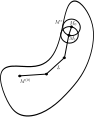
\includegraphics[scale=1.5]{figLaplaceMax.pdf}
\end{figure}

Нетрудно убедиться, что если область $T$ связная и максимальное значение достигается хотя бы в одной внутренней точке $M_0$, то $u(M) \equiv u(M_0)$ во всей области. Пусть $M^{(0)}$ --- какая-либо другая точка области $T$. Соединим точку $M^{(0)}$ с точкой $M_0$ ломаной линией $L$, длину которой обозначим $l$. Пусть $M_1$ есть последняя точка выхода линии $L$ из $\Sigma_{\rho^m}$. В этой точке $u(M_1) = u(M_0)$. Опишем из этой точки сферу $\Sigma_{\rho^m}$ радиуса $\rho_1^m$, касающуюся $\Sigma$, и пусть $M_2$ --- последняя точка выхода $L$ из $\Sigma_{\rho_1^m}$; в этой точке $u(M_2) = u(M_0)$. Продолжая этот процесс далее получим, что не более чем через $p = l / \rho^{(m)}$ шагов, где $\rho^{(m)}$ --- минимальное расстояние от $L$ до $\Sigma$, одна из этих сфер захватит точку $M^{(0)}$, откуда следует, что $u(M^{(0)}) = u (M_0)$. В силу произвольности $M^{(0)}$ и непрерывности $u(M)$ в замкнутой области $T + \Sigma$, заключаем, что $u(M) \equiv u (M_0)$ всюду, включая точки границы. Таким образом, из всех гармонических функций только постоянная может достигать своего максимального значения во внутренних точках области.
\end{qproof}
 \newpage
	
	\subsection{Формулы Грина}\label{que:19}
		Интегральное представление гармонических функций является основным аппаратом для изучения свойств гармонических функций. Одним из важнейших следствий интегральной формулы является принцип максимального значения, часто используемый при решении краевых задач и доказательстве теоремы единственности. \\

\subsubsection{Вывод формул}
Формулы Грина являются прямым следствием формулы Остроградского.
	Формула Остроградского в простейшем случае имеет вид

\begin{equation}
	\iiint\limits_W \derp{R}{z}{}\, dx\, dy\, dz = \iint\limits_S R \cos \gamma\, d\sigma
	\label{equ:equOstrograd}
\end{equation}
где $W$ -- некоторый объём, ограниченный достаточно гладкой поверхностью $S$, $R(x, y, z)$ -- произвольная функция, непрерывная внутри $W + S$ и имеющая непрерывные производные внутри $W$, $\gamma$ -- угол между направлением оси $z$
 и внешней нормалью к $S$. В справедливости этой формулы нетрудно убедиться, проинтегрировав по $z$.\\

    Формулу Остроградского обычно записывают в виде
\begin{equation}
	\iiint\limits_W\left( \derp{a_x}{x}{} + \derp{a_y}{y}{} + \derp{a_z}{z}{}\right) \, d \tau = \iint\limits_S \left\{ a_x \cos \alpha + a_y \cos \beta + a_z \cos \gamma \right\} \, d \sigma
	\label{equ:equOstrograd2}
\end{equation}

	Если $a_x, a_y, a_z$ рассматривать как компоненты некоторого вектора $A = a_x i + a_y j + a_z k$, то формулу Остроградского \eqref{equ:equOstrograd2} можно записать следующим образом
\begin{equation} 
	\iint\limits_W \mathrm{div} \, A \, d \tau = \iint\limits_S A_n \, d \sigma
	\label{equ:equOstrograd3}
\end{equation}
где
 \[
	\mathrm{div}  \bar A = \derp{a_x}{x}{} + \derp{a_y}{y}{} + \derp{a_z}{z}{}
\]
и
\[	
	A_n = a_x \cos \alpha + a_y \cos \beta + a_z \cos \gamma
\]
-- составляющая вектора $A$ вдоль внешней нормали.\\

Перейдём к выводу формул Грина.\\
Пусть $u = (x, y, z)$ и $v = v(x, y, z)$ -- функции. непрерывные вместе со своими первыми производными внутри $W + S$ и имеющие непрерывные вторые производные внутри $W$.

Полагая
\[
	a_x = u \derp{v}{x}{} \quad	a_y = u \derp{v}{y}{} \quad a_z = u \derp{v}{z}{}
\]
и пользуясь формулой Остроградского \eqref{equ:equOstrograd3}, приходим к так называемой \textit{первой формуле Грина}
\begin{equation}
	\iiint\limits_W u \Delta v \, d\tau = \iint\limits_S \derp{v}{n}{} \, d \sigma - \iiint\limits_W \left( \derp{u}{x}{} \derp{v}{x}{} + \derp{u}{y}{} \derp{v}{y}{} + \derp{u}{z}{} \derp{v}{z}{}\right)\, d \tau
\end{equation}
где $\Delta = \derp{}{x}{2} + \derp{}{y}{2} + \derp{}{z}{2}$ -- оператор Лапласа, $\derp{}{n}{} = \cos \alpha \derp{}{x}{} + \cos \beta \derp{}{y}{} + \cos \gamma \derp{}{z}{}$ -- производная по направлению внешней нормали.
	Если учеcть соотношение
\[
	\mathrm{grad}\,u\, \mathrm{grad}\, v = \nabla u \cdot \nabla v = \derp{u}{x}{} \derp{v}{x}{} + \derp{u}{y}{} \derp{v}{y}{} + \derp{u}{z}{} \derp{v}{z}{}
\]
то формулу Грина можно представить в виде
\[
	\iiint\limits_W u \Delta v \, d \tau = - \iiint\limits_W \nabla u \nabla v \, d \tau + \iint\limits_S u \derp{v}{n}{} \, d \sigma
\]
Меняя местами функции $u$ и $v$, будем иметь
\[
	\iiint\limits_W v \Delta u \, d \tau = - \iiint\limits_W \nabla v \nabla u \, d \tau + \iint\limits_S v \derp{u}{n}{} \, d \sigma
\]
Вычитая эти равенства, получаем \textit{вторую формулу Грина}
\begin{equation}
			\iint\limits_S \left(u \der{v}{n}{} - v \der{u}{n}{}\right) d\sigma = \iiint\limits_{W} \left(u \Delta v - v \Delta u \right) d \tau
	\label{equ:Green1}
\end{equation}\\
%\[
%	\bar A = u \left(\derp{v}{x}{} \vec i + \derp{v}{y}{} \vec j + \derp{v}{z}{} \vec k \right) - v \left(\derp{v}{x}{} \vec i + \derp{v}{y}{} \vec j + \derp{v}{z}{} \vec k \right) =			\left(u \derp{v}{x}{} - v \derp{u}{x}{} \right) \vec i + \left(u \derp{v}{y}{} - v \derp{u}{y}{} \right) \vec j + \left(u \derp{v}{z}{} - v \derp{u}{z}{} \right) \vec k
%\]
%\[
%	div A = \derp{}{x}{} \left(u \derp{v}{x}{} - v \derp{u}{x}{} \right) \vec i + \derp{}{y}{} \left(u \derp{v}{y}{} - v \derp{u}{y}{} \right) + \derp{}{z}{} \left(u \derp{v}{z}{} - v \derp{u}{z}{} \right) = 			u \left( \derp{v}{x}{2} + \derp{v}{y}{2} + \derp{v}{z}{2}\right) - v  \left( \derp{u}{x}{2} + \derp{u}{y}{2} + \derp{u}{z}{2}\right) + \derp{u}{y}{}\derp{v}{x}{} - \derp{v}{x}{} \derp{u}{y}{} + \derp{u}{y}{} \derp{v}{y}{} - \derp{v}{y}{} \derp{u}{y}{} + \derp{u}{z}{} \derp{v}{z}{} - \derp{u}{z}{} \derp{v}{z}{}
%\]
		%Получили формулы Грина:\\
Основная интегральная формула Грина
\begin{equation}
	\Omega \cdot u(A) = \iint\limits_S \left[ \frac{1}{R_{AP}} \derp{u(P)}{n_P}{}  - u (P) \derp{}{n_P}{} \left( \frac{1}{R_{AP}} \right) \right] d\sigma_P - \iiint\limits_W \frac{\Delta u (P)}{R_{AP}}\, d\tau_P
	\label{equ:equMainGreen3d}
\end{equation}
где $\Omega$ принимает значения 

\[
	\Omega = \begin{cases}
		4 \pi &\mbox{если точка}\, A\, \mbox{лежит внутри}\, W\\
		2 \pi &\mbox{если точка}\, A\, \mbox{лежит на границе}\, S\\
		0 & \mbox{если точка}\, A\, \mbox{лежит вне}\, W
	\end{cases}
\]


Аналогичная формула существует и для гармонических функций двух независимых переменных. 
Пусть $S$ -- область на плоскости $(x, y)$, ограниченная контуром $C$, а $n$ -- направление нормали к этому контуру, внешнее по отношению к области $S$.

Полагая во второй формуле Грина $v = \ln \frac{1}{R_{AP}}$, где $R_{AP} = \sqrt{ (x - x_0)^2 + (y - y_0)^2}$ -- расстояние $P$ от $A$, получаем 
\begin{equation}
	\Omega \cdot u(A) = \int\limits_S \left[ \ln \frac{1}{R_{AP}} \derp{u(P)}{n_P}{}  - u (P) \derp{}{n_P}{} \left( \ln \frac{1}{R_{AP}} \right) \right] dS_P - \iint\limits_S \frac{\Delta u (P)}{\ln R_{AP}}\, dS_P
	\label{equ:equMainGreen2d}
\end{equation}
где $\Omega$ принимает значения 

\[
	\Omega = \begin{cases}
		2 \pi &\mbox{если точка}\, A\, \mbox{лежит внутри}\, S\\
		\pi &\mbox{если точка}\, A\, \mbox{лежит на границе}\, C\\
		0 & \mbox{если точка}\, A\, \mbox{лежит вне}\, S
	\end{cases}
\]


\subsubsection{Метод Грина для задачи Дирихле в трёхмерном случае}\label{que:25}
	Вторая формула грина:
\[ 
			\iint\limits_S \left(u \der{v}{n}{} - v \der{u}{n}{}\right) d\sigma = \iiint\limits_{W} \left(u \Delta v - v \Delta u \right) d \tau
\]
Рассмотрим трёхмерную задачу Дирихле. 
\[
	\Delta u = 0
\]
\[
	u\big|_S = f
\]
\begin{wrapfigure}{r}{0.3\textwidth}
	\centering
	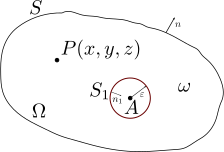
\includegraphics[width = 0.3\textwidth]{figGreenThreeDim.pdf}
\end{wrapfigure}
Применим вторую формулу Грина к этой задаче.\\

В области $\Omega$ возьмём $(\cdot)A(x_0, y_0, z_0)$ и произвольную $(\cdot)P(x, y, z)$.
\[
	r_{AP} = \sqrt{(x - x_0)^2 + (y - y_0)^2 + (z - z_0)^2}\quad \text{радиус между $A$ и $P$}
\]
Покажем, что $w = \frac{1}{r_{AP}}$ удовлетворяет уравнению Лапласа $\Delta u = 0$:
\[
	\Delta u = \derp{u}{x}{2} + \derp{u}{y}{2} + \derp{u}{z}{2} = 0
\]
Найдём вторые производные и подставим в уравнение:
\[
	\derp{w}{x}{} = - \frac{1}{r_{AP}^2} \derp{r_{AP}}{x}{} = - \frac{1}{r_{AP}^2} \frac{ (x - x_0)}{  \sqrt{(x - x_0)^2 + (y - y_0)^2 + (z - z_0)^2}} = - \frac{(x - x_0)}{r_{AP}^3}
\]
\begin{align*}
	\derp{w}{x}{2} &= - \frac{1}{r_{AP}^3} + \frac{3 (x - x_0)}{r_{AP}^5}\\
	\derp{w}{y}{2} &= - \frac{1}{r_{AP}^3} + \frac{3 (y - y_0)}{r_{AP}^5}\\
	\derp{w}{z}{2} &= - \frac{1}{r_{AP}^3} + \frac{3 (z - z_0)}{r_{AP}^5}
\end{align*}
\[
	\Delta u - \frac{3}{r_{AP}^3} + \frac{3 [(x - x_0)^2 + (y - y_0)^2 + (z - z_0)^2]}{r_{AP}^5} \equiv 0
\]
Действительно $w = \frac{1}{r_{AP}}$ удовлетворяет уравнению Лапласа, то есть является гармонической.\\[5pt]
Должное решение в $(\cdot)A$ имеет особенность. Окружаем $(\cdot)A$ сферой малого радиуса $\varepsilon$. $w$ --- область между двумя сферами. Тогда формула Грина принимает вид:
\[
	\iint\limits_S \left(u \der{v}{n}{} - v \der{u}{n}{}\right) dS + \iint\limits_{S_1} \left(u \der{v}{n_1}{} - v \der{u}{n_1}{}\right) dS_1 = \iiint\limits_\omega \left(u \Delta v - v \Delta u \right) d \omega
\]

Функция $w$  в области $\omega$ не имеет особенностей. Во всей области строим решение $w_1$, которое имеет особенность. 

Потребуем, чтобы $\Delta w_1 = 0; w_1 \big|_S = W\big|_S$. Построим функцию Грина:
\[
	G(x, y, z, x_0, y_0, z_0) = w_1 - w
\]
Тогда на границе: 
\[
	G\big|_S = 0
\]
Предположим, что в формуле Грина $v = G$.
\[
	\iint\limits_S \left(u \der{v}{n}{} - v \underbrace{\der{u}{n}{}}_0\right) dS + \iint\limits_{S_1} \left(u \der{v}{n_1}{} - v \der{u}{n_1}{}\right) dS_1 = 0
\]
Получаем 
\[
	\iint\limits_S u \derp{G}{n}{}\, dS + \iint\limits_{S_1} \left(u \der{G}{n_1}{} - G \der{u}{n_1}{}\right) dS_1 = 0
\]

\begin{wrapfigure}{l}{0.3\textwidth}
	\centering
	\includegraphics[width = 0.3\textwidth]{figGreenIllust.pdf}
\end{wrapfigure}
Перейдём к сферической системе координат во втором интеграле:
\begin{align*}
	&dS_1 = \varepsilon^2 \sin \theta\, d \theta d \varphi\\
	&0 \leqslant \theta \leqslant \pi; \quad 0 \leqslant \varphi \leqslant 2\pi\\
	&\derp{}{n_1}{} = - \derp{}{r}{}
\end{align*}

\[
	 \iint\limits_{S_1} \left(u \der{G}{n_1}{} - G \der{u}{n_1}{}\right) dS_1 = \int\limits_0^{2 \pi}\, d\varphi \int\limits_0^{\pi} \left(- u \der{G}{r}{} + G \der{u}{r}{} \right) \varepsilon \sin \theta\, d\theta
\]
\[
	G = w_1 - \frac{1}{r_{AP}}
\]
\begin{multline*}
	\iint\limits_{S_1} \left(u \derp{G}{n_1}{} - G \derp{u}{n_1}{} \right)\, dS = \iint\limits_{S_1} \Big(- u \derp{}{r}{} \Big(w_1 - \frac{1}{\underbrace{r_{AP}}_r} \Big) + \Big(w_1 - \frac{1}{\underbrace{r_{AP}}_r} \Big) \derp{u}{r}{} \Big)\, dS =\\
	= \iint\limits_{S_1} \left(- u \derp{w_1}{r}{} - \frac{1}{r^2} u + w_1 \derp{u}{r}{} - \frac{1}{r} \derp{u}{r}{}\right)\, dS = \\
	= \int\limits_0^{2 \pi}d \varphi \int\limits_0^\pi d \theta \left\{ - u \derp{w_1}{r}{} - \frac{1}{\varepsilon^2} u + w_1 \derp{u}{r}{} - \frac{1}{\varepsilon} \derp{u}{r}{} \right\} \varepsilon^2 \sin \theta
\end{multline*}

Будем устремлять радиус $\varepsilon$ к $0$:
\[
	\lim\limits_{\varepsilon \to 0} \iint\limits_{S_1} \left(u \derp{G}{n_1}{} - G \derp{u}{n_1}{} \right)\, dS = \lim\limits_{\varepsilon \to 0} \varepsilon^2 \int\limits_0^{2 \pi} d\varphi \int\limits_0^{2 \pi} d \theta \sin \theta \left\{ - u \derp{w_1}{r}{} - \frac{1}{\varepsilon^2} u + w_1 \derp{u}{r}{} - \frac{1}{\varepsilon} \derp{u}{r}{} \right\}
\]
\[
	\varepsilon^2 u \derp{w}{r}{} \to 0 \big|_{\varepsilon \to 0}
\]
\[
	\varepsilon^2 w_1 \derp{u}{r}{} \to 0; \quad \varepsilon \derp{u}{r}{} \to 0
\]
Получаем 
\[
	- \int\limits_0^{2 \pi} d \varphi \int\limits_0^\pi d\theta \sin \theta u - u(x_0, y_0, z_0) \int\limits_0^{2 \pi} d \varphi \int\limits_0^\pi \sin \theta = - 4 \pi u (x_0, y_0, z_0)
\]
Подставляем в формулу Грина:
\[
	\iint\limits_S u \derp{G}{n}{}\, dS - 4 \pi u (x_0, y_0, z_0) = 0
\]
\[
	u (x_0, y_0, z_0) = \frac{1}{4 \pi} \iint\limits_S f \derp{G}{n}{}\, dS
\]




\subsubsection{Метод Грина для задачи Дирихле в двумерном случае}\label{que:26}
	\[	
	u(x_0, y_0, z_0) = \iint\limits_S \left(u \derp{G}{n}{} - G \derp{u}{n}{} \right)\, dS + \iiint\limits_\Omega F \, d\Omega = \begin{cases}
		2 \pi u &A \in \Omega\\
		\pi u & A \in S\\
		0 &  A\notin \Omega\\
	\end{cases}
\]
где $F(x, y, z) = \Delta u$.\\

В плоском случае фундаментальным решением задачи Лапласа является $\ln \frac{1}{r}$.
Рассмотрим задачу.
\[
	\Delta u = 0
\]
\[
	\derp{u}{x}{2} + \derp{u}{y}{2} = 0
\]
\[
	r= \sqrt{(x - x_0)^2 + (y - y_0)^2}
\]
\[
	u = \ln \frac{1}{r} = - \ln r
\]
\begin{align*}
	&\derp{u}{x}{} = - \frac{1}{r} \cdot \derp{r}{x}{} = - \frac{1}{r^2 (x - x_0)}\\
	&\derp{u}{x}{2} = - \frac{1}{r^2} + \frac{2  (y - y_0)^2}{r^4}\\
	&\derp{u}{x}{2} + \derp{u}{y}{2} = -\frac{2}{r^2} + \frac{2 \left[ (x - x_0)^2 + (y - y_0)^2 \right]}{r^4} = - \frac{2}{r^2} + \frac{2}{r^2} = 0
\end{align*}
\[	
	\Delta G = 0
\]
\[
	G\big|_\Gamma = 0
\]
\[
	G = W - \ln \frac{1}{r_AP} 
\]
\[
	\oint\limits_\Gamma \left(u \derp{v}{n}{} - v \derp{u}{n}{} \right)\, d \gamma = \iint\limits_S \left(u \Delta - v \Delta u \right)\, dS
\]
Радиус окружности $\Gamma_1 = \varepsilon$.
\begin{figure}[h!]
	\centering
	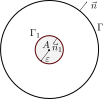
\includegraphics{figGreenMethTwoDim.pdf}
\end{figure}
\[
	\oint\limits_\Gamma \left(u \derp{v}{n}{} - v \derp{u}{n}{} \right)\, d\gamma + \oint\limits_{\Gamma_1} \left(u \derp{v}{n_1}{} - v \derp{u}{n_1}{} \right)\, d\gamma = 0
\]
\[
	v = G
\]
Нас интересует интеграл вида
\[
	\oint\limits_{\Gamma_1} \left(u \derp{G}{n_1}{} - G \derp{u}{n_1}{} \right)\, d\gamma
\]
Если интеграл берётся по окружности радиуса $\varepsilon$, то:
\[
	\derp{}{n_1}{} = - \derp{}{r}{}, \qquad dr = \varepsilon\, d\theta
\]
\[
	\iint\limits_0^{2\pi} \left( - u \derp{G}{r}{} + G \derp{u}{r}{} \right) \varepsilon d\theta = \int\limits_0^{2\pi} \left(- u \derp{w}{r}{} + w \derp{u}{r}{} + u \derp{}{r}{} \left(\ln \frac{1}{r} \right) - \ln \frac{1}{r} \derp{u}{r}{}\right) \cdot \varepsilon
\]
\[
	(- \ln r )' = - \frac{1}{r}
\]
Перейдём к пределу:
\[
	\lim\limits_{\varepsilon \to 0} \oint\limits_{\Gamma_1} \left(u \derp{G}{n_1}{} - G \derp{u}{n_1}{} \right) = \\ 
	=	\lim\limits_{\varepsilon \to 0} \int\limits_0^{2 \pi} \left(- u \derp{w}{r}{} + w \derp{u}{r}{} \right)\, d\theta - \lim\limits_{\varepsilon \to 0} \varepsilon \int\limits_0^{2 \pi} \left[u \frac{1}{\varepsilon}  + \derp{u}{r}{} \ln \varepsilon\right]\, d\theta  
\]
Так как $u, w$ --- непрерывно гладкие функции, то
\[
	\varepsilon \ln \varepsilon \underset{\varepsilon \to 0}{\to} 0
\]

В итоге получаем 
\[
	- \int\limits_0^{2 \pi} u \, d \theta
\]
Значит:
\[
	\oint\limits_\Gamma \left(u \derp{v}{n}{} - v \derp{u}{n}{} \right)\, d\gamma - \underbrace{\int\limits_0^{2 \pi} u\, d \theta}_{u(x_0, y_0) 2 \pi} = 0
\]
так как интегрируем в малой области.



   \newpage

	\subsection{Функция источника}
			Метод функции источника даёт удобный аппарат для аналитического представления решения краевых задач. 

	
		\subsubsection{Функция источника для уравнения $\Delta u = 0$ и её основные свойства.}
			Для всякой функции $u$, непрерывной вместе с первыми производными в замкнутой области $W$, ограниченной достаточно гладкой поверхностью $S$, и имеющей вторые производные внутри $W$, имеет место представление
\begin{equation}
	u(M_0) = \frac{1}{4 \pi} \iint\limits_{S} \left[ \frac{1}{R_{PA}} \derp{u}{n}{} - u(P) \derp{}{n}{} \left(\frac{1}{R_{PA}} \right) \right]\, d\sigma_p - \frac{1}{4 \pi} \iiint\limits_W \frac{\Delta u}{R_{MA}}\, d\tau_M.
\end{equation}

Если функция $u(A)$ гармоническая, то объёмный интеграл равен нулю; если же $u(A)$ удовлетворяет уравнению Пуассона, то объёмный интеграл является известной функцией.

Пусть $v(A)$ -- некоторая гармоническая функция, непрерывная в $W + S$ вместе с первыми производными, не имеющая нигде особенностей. Вторая формула Грина даёт
\begin{equation}
	0 = \iint\limits_S \left( v \derp{u}{n}{} - u \derp{v}{n}{} \right) \, d\sigma - \iiint\limits_W v \Delta u \, d \sigma
	\label{equ:equGreen2Trans}
\end{equation}

Складывая основную формулу Грина \eqref{equ:equMainGreen3d} и \eqref{equ:equGreen2Trans} получаем
\begin{equation}
	u(A) = \iint\limits_S \left[ G \derp{u}{n}{} - u \derp{G}{n}{}\right] \, d\sigma -  \iiint\limits_W \Delta u \cdot G \, d \tau
	\label{equ:equSourceFunction}
\end{equation}
где
\begin{equation}
	G(M, M_0) = \frac{1}{4 \pi R_{AP}} + v
	\label{equ:equSourceFunction2}
\end{equation}
-- функция двух точек. Точка $A$ фиксирована, и поэтому $x, y, z$ играют роль параметров.\\

Формула \eqref{equ:equSourceFunction} содержит $u\big|_S$ и $\left. \derp{u}{n}{} \right|_S$. При решении первой краевой задачи задаётся лишь $u\big|_S$, а при решении второй -- значение $\left. \derp{u}{n}{} \right|_S$. Функция $v$ выбирается таким образом, чтобы $G|_S = 0$ для первой краевой задачи $\left(\left. \derp{u}{n}{} \right|_S = 0 \: \mbox{для второй краевой задачи}\right)$. Определим функцию $G(A, P)$ при помощи условий:
\begin{enumerate}
	\item $G(A, P)$ как функция точки $P(\xi, \eta, \sigma)$ при фиксированной точке $A(x, y, z)$ удовлетворяет уравнению Лапласа
	\[
		\Delta G = G_{\xi \xi} + G_{\eta \eta} + G_{\sigma \sigma} = 0, \quad P \neq A
	\]
	во всех точках $P$ области $W$, кроме точки $P = A$.
	\item $G(A, P)$ при совпадении аргументов $(A = P)$ обращается в бесконечность и представима в виде \eqref{equ:equSourceFunction2}, где $v = v (A, P)$ -- гармоническая всюду в $W$ функция.
	\item $G(A, P)$ на границе обращается в нуль:
	\[
		G(A, P) = 0, \quad \mbox{если}\quad  P \in S
	\]
	Этому условию можно удовлетворить, потребовав, чтобы 
	\[
		v\big|_S = - \frac{1}{4 \pi R}
	\]
\end{enumerate}

Функцию $G$, определённую таким образом, будем называть \textit{функцией точечного источника первой краевой задачи для уравнения $\Delta u = 0$.} В самом деле, формула \eqref{equ:equSourceFunction} даёт:
\begin{equation}
	u(A) = - \iint\limits_S u \derp{G}{n}{}\, d\sigma = - \iint\limits_S f \derp{G}{n}{}\, d\sigma \quad (f = u\big|_s)
	\label{equ:equSourceFunction3}
\end{equation}
Формула \eqref{equ:equSourceFunction3} построена с помощью формулы Грина, предполагающей выполнение определённых условий в отношении функций $u$ и $G$ и поверхности $S$. В формулу  \eqref{equ:equSourceFunction3} входит выражение $\derp{G}{n}{}$, существование которого на поверхности $S$ не следует непосредственно из определения функции $G$.
%\[
%	\Delta u = 0 \quad u \in W
%\]
%\[
%	u|_s = f
%\]

%\[
%	W = \frac{1}{r_{AP}}
%\]
%где $
%	r_{AP} = \sqrt{(x - x_0)^2 + (y - y_0)^2 + (z - z_0)^2}
%$
%-- расстояние между точками $A(x, y, z)$ и $P (x_0, y_0, z_0)$.
%\begin{align*}
%	 &\derp{W}{x}{} = - \frac{1}{r_{AP}^2} \derp{r_{AP}}{x}{} = - \frac{1}{r_{AP}^2} \frac{2 (x - x_0)}{2 \sqrt{(x - x_0)^2 + (y - y_0)^2 + (z - z_0)^2}} = \frac{(x - x_0)}{r_{AP}^3}\\[10pt]
%	&\derp{W}{x}{2} = - \frac{1}{r_{AP}^3} + \frac{3 (x - x_0)^2}{r_{AP}^5}; \quad \derp{W}{y}{2} = - \frac{1}{r_{AP}^3} + \frac{3 (y - y_0)^2}{r_{AP}^5}; \quad \derp{W}{z}{2} = - \frac{1}{r_{AP}^3} + \frac{3 (z - z_0)^2}{r_{AP}^5}; 
%\end{align*}
%\[
%	\Delta u = - \frac{3}{r_{AP}^3} + \frac{3 [(x - x_0)^2 + (y - y_0)^2 + (z - z_0)^2]}{r_{AP}^5} = 0
%\]
%		Данное решение имеет в точке $A$ особенность.\\
%\[
%	\iint\limits_{S} \left(u \derp{v}{n}{} - v \derp{u}{n}{}\right) dS = \iint\limits_S \left(u \der{v}{n}{} - v \der{u}{n}{}\right) dS = \iiint\limits_{W} \left(u \Delta v - v \Delta u \right) d \omega
%\]
%		Решение $W = \frac{1}{r_{AP}}$ верно только в области $\omega$. Попробуем построить решение $W_1$ для всей области $W$.\\
%		
%		Построим функцию Грина\\
%\[
%	\Delta W_1 = 0 \quad W_1 |_S = W |_S
%\]
%\[
%	G (x, y, z, x_0, y_0, z_0) = W_1 - W; \quad G|_S = 0
%\]
%		Предположим, что в функции Грина $v = G$. Тогда 
%\[
%	\iint\limits_{S} \left(u \derp{v}{n}{} - v \derp{u}{n}{}\right) dS = \iint\limits_S \left(u \der{v}{n}{} - v \der{u}{n}{}\right) dS = \iiint\limits_{W} \left(u \Delta v - v \Delta u \right) d \omega
%\] %подписать что равно нулю
%\[
%	\iint\limits_{S} \left(u \derp{G}{n}{} \right) dS + \iint\limits_{S_1} \left(u \der{G}{n_1}{} - v \der{u}{n_1}{}\right) dS_1 = 0 
%\]
%		Перейдём к сферической системе координат.\\
%\begin{figure}[h!]
%	\centering
%	\includegraphics{figGreenIllust.pdf}
%\end{figure}
%\[
%	dS_1 = \varepsilon^2 \sin \theta \, dv d \varphi
%\]
%\[
%	\iint\limits_{S_1} \left(u \der{G}{n_1}{} - v \der{u}{n_1}{}\right) dS_1 = \int\limits_0^{2 \pi} d\varphi \int\limits_0^{\pi} \left(- u \der{G}{r}{} + G \der{u}{r}{} \right) \varepsilon \sin \theta d \theta
%\]

%\begin{multline*}
%	\lim\limits_{\varepsilon \to 0} \iint\limits_{S_1} \left( u \derp{G}{u_1}{} - G \derp{u}{u_1}{} \right) ds = - \int\limits_{0}^{2 \pi} d \varphi \int\limits_{0}^{\pi} d\theta \sin \theta u = \\ = u (x_0, y_0, z_0)\int\limits_0^{2 \pi} d \varphi \int\limits_{0}^{\pi} \sin \theta d \theta = - 4 \pi u (x_0, y_0, z_0) 
%\end{multline*}
%\[
%	u(x_0, y_0, z_0) = \frac{1}{4 \pi} \iint\limits_S f \derp{G}{u}{} dS
%\]
%Получили решение задачи Дирихле через функцию Грина.\\
%Функцию Грина можно построить для шара, сферы и полупространства.\\


		\subsubsection{Функция источника для круга} \label{que:24}
			\begin{wrapfigure}[0]{R}{0.4\textwidth}
	\centering
	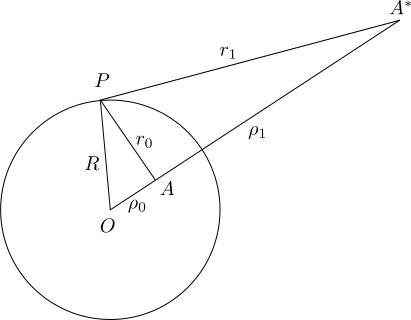
\includegraphics[width=0.4\textwidth]{figSourceFunctionCircle.pdf}
\end{wrapfigure}
\begin{minipage}[t]{0.55\textwidth}
Функция источника для круга может быть получена таким же способом, как и функция для сферы. В этом случае функцию следует искать в виде
\begin{equation}
	G = \frac{1}{2 \pi} \ln \frac{1}{r} + v
	\label{equ:equSourceFunCircle}
\end{equation}
Поместим в точку $A$ единичный заряд и отложим на радиусе, проходящем через точку $A$, такой отрезок $OA^*$, что
\begin{equation}
	\rho_0\rho_1 = R^2,
	\label{equ:SourceFunCircle1}
\end{equation}
гдe $\rho_0 = OA$, $\rho_1 = OA^*$.
Преобразование \eqref{equ:SourceFunCircle1}, ставящее в соответствие точке $A$ определённую точку $A^*$, является преобразованием обратных радиусов, а сама точка $A*$ называется \textit{сопряжённой} с точкой $A$. 
\end{minipage}\\
Докажем, что для всех точек $P$, расположенных на сфере, расстояния до $A$ и $A^*$ пропорциональны.  Для этого рассмотрим треугольники $OPA$ и $OPA^*$; они подобны, так как угол при $O$ общий, а прилежащие к нему стороны пропорциональны:
\[
	\frac{\rho_0}{R}=\frac{R}{\rho_1} \quad \mbox{или} \quad \frac{OA}{R} = \frac{R}{OA^*}
\]
Из подобия треугольников следует:
\begin{equation}
	\frac{r_0}{r_1} = \frac{\rho_0}{R} = \frac{R}{\rho_1},
	\label{equ:SourceFunCircle2}
\end{equation}
где $r_0 = \abs{\overrightarrow{AP}}$, $r_1 = \abs{\overrightarrow{A^*P}}$. Из пропорции \eqref{equ:SourceFunCircle2} получаем:
\[
	r_0 = \frac{\rho_0}{R} r_1
\]
для всех точек круга. Поэтому гармоническая функция $v = - \frac{1}{2 \pi} \ln \frac{R}{\rho_0} \frac{1}{r_1}$ на круге принимает то же значение, что и функция $\frac{1}{r_0}$. Она представляет, очевидно, потенциал заряда величины $- \frac{R}{\rho_0}$ помещённого в точку $A^*$.

Таким образом, функция 
\begin{equation}
 	G(P, A) = \frac{1}{2 \pi} \left[ \ln \frac{1}{r_0} - \ln \frac{R}{\rho_0} \frac{1}{r_1} \right],
\end{equation}
где  $\rho_0 = OA$, $r_0 = AP$, $r_1 = A^*P$, $R = OP$ -- радиус круга.
%\[
%	r_0 \cdot r_* = R^2 \Rightarrow r_* = \frac{R^2}{r_0}
%\]
%\[
%	x_* = \frac{R'}{x_0}; \quad  y_* = \frac{R^2}{y_0}; \quad  z_* = \frac{R^2}{z_0} 
%\]
%\[
%	r_{AP} = \sqrt{(x - x_0)^2 + (y - y_0)^2 + (z - z_0)^2}
%\]
%Составим функцию Грина
%\[
%	G = \frac{B}{r_{A*P}} - \frac{1}{r_{AP}}
%\]
%\[
%	r_{AP} = \sqrt{r^2 + r_0^2 - 2 r r_0 \cos \xi}
%\]
%\[
%	r_{A*P} = \sqrt{r^2 + r_*^2 - 2 r r_* \cos \xi}
%\]
%

Нетрудно убедиться в том, что определённая таким образом гармоническая функция обращается в нуль на границе
\[
	G|_{r = R} = 0
\]
%\[
%	r_{AP}|_{r = R} = \sqrt{R^2 + r_0^2 - 2 R r_0 \cos \xi}
%\]
%\[
%	r_{A*P}|_{r = R} = \sqrt{R^2 + \frac{R^4}{r_0^2} - 2 R \frac{R^2}{r_0} \cos \xi} = \frac{R}{r_0} \sqrt{r_0^2 + R^2 - 2 R r_0 \cos \xi} = \frac{R}{r_0} r_{AP}
%\]
Для решения краевой задачи надо вычислить значения $\derp{G}{n}{}$ на окружности $C$.
%\[
%	\frac{B}{\frac{R}{r_0} r_{AP}} - \frac{1}{r_{AP}} = 0; \quad B = \frac{R}{r_0}
%\]
%\begin{multline*}
%	\left. \derp{G}{u}{} \right|_{r = R} = \left.\derp{G}{r}{}\right|_{r = R} = \left[\frac{R}{r_0} \left( - \frac{1}{r_{A*P}^2} \right) \derp{r_{A*P}}{r}{} + \frac{1}{r_{AP}^2} \derp{r_{AP}}{r}{} \right] |_{r = R} = \\ = \left[ - \frac{R(r - r_* \cos \xi)}{r_0 r_{AP}^3} + \frac{1}{r_{AP}^3} (r - r_0 \cos \xi) \right]_{r = R} = \\ = \frac{-R^2 + \frac{R^3}{r_0} \cos \xi}{r_0 \frac{R^3}{r_0^3} r_{AP}^3} + \frac{R - r_0 \cos \xi}{r_{AP}^3} = \frac{1}{r_{AP}^3} \left[ - \frac{r_0^3}{R} + r_0 \cos \xi + R - r_0 \cos \xi \right]
%\end{multline*}
\[
	\left.\derp{G}{n}{}\right|_C = - \frac{1}{2 \pi R} \frac{R^2 - \rho_0}{r_0^2}.
\]
Пусть $(\rho, \theta)$ -- полярные координаты точки $P$, лежащей на окружности, а $(\rho, \theta_0)$ -- координаты точки $A$, тогда
\[
	r_0^2 = R^2 + \rho_0^2 - 2 R \rho_0 \cos (\theta - \theta_0).
\]
Подставляя в формулу 
\[
	u(\rho_0, \theta_0) = \frac{1}{2 \pi} \int\limits_C u(P) \frac{R^2 - \rho_0^2}{r_0^2} \frac{ds}{R}
\]
это выражение для $r_0$ и принимая во внимание, что 
\[
	u(P) \big|_C = f(\theta) \quad \mbox{и} \quad ds = R\, d\theta
\]
%\[
%	u(x_0, y_0, z_0) = \frac{1}{4 \pi} \iint\limits_S f(\theta) \cdot \frac{(R^2 - r_0^2)}{R(R^2 + r_0^2 - 2 R r_0 \cos \psi)^{\frac{3}{2}}}\, d \theta
%\]
%\[
%	u(r_0, \theta_0, \varphi_0) = \frac{1}{4 \pi} \int\limits_0^{2 \pi} d\varphi \int\limits_0^{\pi} f \frac{(R^2 - r_0^2) R^2 \sin \theta d \theta}{R (R^2 + r_0^2 - 2 R r_0 \cos \xi)^{\frac{3}{2}}}
%\]

%\[
%	\overline{OA} = x_0 \bar i + y_0 \bar j + z_0 \bar k = r_0 \sin \theta _0 \cos \varphi_0 \bar i + r_0 \sin \theta_0 \sin \varphi_0 \bar j + r_0 \cos \theta_0 \bar k
%\]
%\[
%	\overline{OP} = x \bar i + y \bar j + z \bar k = r (\sin \theta \cos \varphi \bar i + \sin \theta \sin \varphi %\bar j + \cos \theta \bar k)
%\]
%\[
%	\frac{\overline{OA}}{\abs{OA}} = \frac{\overline{OA}}{r_0} = \bar e (\sin \theta_0 \cos \varphi_0, \sin %\theta_0 \sin \varphi_0, \cos \theta_0)
%\]
%\[
%	\frac{\overline{OP}}{\abs{OP}} = \frac{\overline{OP}}{\bar r} = \bar e (\sin \theta \cos \varphi, \sin \theta \sin \varphi \cos \theta)
%\]

приходим для функции $u(A)$ к выражению 
\begin{equation}
	u(\rho_0, \theta_0) = \frac{1}{2 \pi} \int\limits_0^{2 \pi} \frac{R^2 - \rho_0^2}{R^2 + \rho_0^2 - 2 R \rho_0 \cos (\theta - \theta_0)} f(\theta) \, d \theta
	\label{equ:equSourceFunctionCircle}
\end{equation}
называемому \textit{интегралом Пуассона для круга}. Эта же формула с точностью до знака даёт решение внешней задачи.
 \newpage

		\subsubsection{Функция источника для полупространства}
			Понятие функции источника и формула \eqref{equ:equSourceFunction3} имеют место и для неограниченного пространства, если рассматривать функции, регулярные на бесконечности. Найдём функцию источника для полупространства $z > 0$. Поместим в точку $A(x_0, y_0, z_0)$ единичный заряд, который создаёт в неограниченном пространстве поле, потенциал которого определяется функцией
\begin{equation}
	\frac{1}{4 \pi} \frac{1}{R_{AM}}, \quad \mbox{где} \quad R_{AM} = \sqrt{(x - x_0)^2 + (y - y_0)^2 + (z - z_0)^2}
	\label{equ:equSourceFunHalfSpat}
\end{equation}

\begin{figure}[h!]
	\centering	
	\includegraphics[scale=1]{figHalfSpatial.pdf}
\end{figure}
Нетрудно видеть, что <<индуцированное поле>> $v$  является полем отрицательного единичного заряда, помещённого в точку $M_1 (x_0, y_0, - z_0)$, являющуюся зеркальным изображением точки $M_0$ в плоскости $z = 0$. Функция $G$, равная 
\[
	G(M, A) = \frac{1}{4 \pi R_0} - \frac{1}{4 \pi R_1}
\]
где 
\begin{align}
	R_0 = \abs{\overrightarrow{AM}} &= \sqrt{(x - x_0)^2 + (y - y_0)^2 + (z - z_0)^2}\\
	R_1 = \abs{\overrightarrow{M_1M}} &= \sqrt{(x - x_0)^2 + (y - y_0)^2 + (z + z_0)^2}
\end{align}
обращается в нуль при $z = 0$ и имеет ненужную особенность в точке $A$.

Вычислим $\left. \derp{G}{n}{}\right|_{z = 0} = - \left. \derp{G}{z}{}\right|_{z = 0}$. Очевидно, что
\[
	\derp{G}{z}{} = \frac{1}{4 \pi} \left[ - \frac{z - z_0}{R_0^3} + \frac{z + z_0}{R_1^3} \right].
\]
Полагая $z = 0$, находим:
\[
	\left. \derp{G}{n}{} \right|_{z = 0} = \left. - \frac{G}{z}\right|_{z = 0} = - \frac{z_0}{2 \pi R_0^3}.
\]
Решение первой краевой задачи даётся формулой 
\[	
	u(A) = \frac{1}{2 \pi} \iint\limits_S \frac{z_0}{R_{AP} }f(p)\, d\sigma_P
\]
где $S$ -- плоскость $z = 0$, $f(P) = u|_{z = 0}$, или
\[
	u(x_0, y_0, z_0) = \frac{1}{2 \pi} \int\limits_{-\infty}^{\infty} \int\limits_{- \infty}^{\infty} \frac{z_0}{\left[(x - x_0)^2 + (y - y_0)^2 + z_0^2 \right]^{\frac{3}{2}}} f(x, y)\, dx dy
\]
%Для данной задачи мы должны построить функцию Грина.
%\[
%	G = W - \frac{1}{r_{AP}} = \frac{B}{r_{AP} - \frac{1}{r_{AP}}}
%\]
%\[
%	G|_{z = 0} = \left(\frac{B}{r_{AP} - \frac{1}{r_{AP}}} \right)_{z = 0} = 0
%\]
%\[
%	r_{AP} = \sqrt{(x - x_0)^2 + (y - y_0)^2 + (z - z_0)^2}
%\]
%\[
%	r_{A*P} = \sqrt{(x - x_0)^2 + (y - y_0)^2 + (z + z_0)^2}
%\]
%\[
%	z = 0 \to r_{AP} = r_{A*P}
%\]
%Нормаль направлена в сторону противоположную $z$, следовательно $\derp{G}{n}{} = - \derp{G}{z}{}$
%\[
%	G = \frac{1}{r_{AP}} - \frac{1}{r_{AP}}; - \derp{G}{z}{} = \frac{1}{r_{A*P}^2} \derp{r_{A*P}}{z}{} - \frac{1}{r_{AP}^2} \derp{r_{AP}}{z}{} = \frac{(z + z_0)}{r_{A*P}^3} - \frac{(z - z_0)}{r_{AP}^3} |_{z = 0} = \frac{2 z_0}{r_{AP}^3}
%\]
%Перейдём к формуле Грина \eqref{equ:equMainGreen3d}
	
%\begin{multline*}
%	4 \pi u(x_0, y_0, z_0) = \iint\limits_{S} u \derp{G}{n}{} dS = - \int\limits_{- \infty}^{+ \infty} dx \int\limits_{- \infty}^{+ \infty} dy f(x, y) \derp{G}{z}{} = \\ = - 2 z_0 \int\limits_{- \infty}^{+ \infty} dx \int\limits_{- \infty}^{+ \infty} \frac{f(x,y)}{\left[(x - x_0)^2 + (y - y_0)^2 +z_0^2 \right]^\frac{3}{2}} dy = \\ = [(x - x_0)^2 + (y - y_0)^2 +z_0^2 = x^2 + y^2 + x_0^2 + y_0^2 + z_0^2 - 2x x_0 - 2 y y_0] = \\ = \rho^2 + \rho_0^2 - 2 \rho \rho_0 \cos \theta \cos \theta_0 - 2 \rho \rho_0 \sin \theta \sin \theta_0] = \\ = - 2 z_0 \int\limits_{0}^{2 \pi} d\theta \int\limits_{0}^{\infty} \frac{f(\rho, \theta) \rho d\rho}{[\rho^2 + \rho_0^2 - 2 \rho \rho_0 \cos \theta \cos \theta_0 - 2 \rho \rho_0 \sin \theta \sin \theta_0]^\frac{3}{2}}
%\end{multline*}
%	$\iint\limits_S \left( u \derp{G}{n}{} - G \derp{u}{n}{}\right)dS + \iiint\limits_{\omega} = \begin{cases}
%		4 \pi &\mbox{если точка}\, A\, \mbox{лежит внутри}\, W\\
%		2 \pi &\mbox{если точка}\, A\, \mbox{лежит на границе}\, S\\
%		0 & \mbox{если точка}\, A\, \mbox{лежит вне}\, W
%	\end{cases}$\\

%Для пространственной задачи фундаментальным решением является $	\frac{1}{r}$ \\
%В плоском случае фундаментальным решением является 
%\[
%	\ln \frac{1}{r}
%\]
%\[
%	\Delta u = 0 \quad \derp{u}{x}{2} + \derp{u}{y}{2} = 0
%\]
%\[
%	r = \sqrt{(x - x_0)^2 + (y - y_0)^2}
%\]
%\[
%	u = \ln \frac{1}{r} = - \ln r
%\]
%Найдём производную\\
%\[
%	\derp{u}{x}{} = - \frac{1}{r} \derp{r}{x}{} = - \frac{1}{r^2}
%\]
%\[
%	\derp{u}{x}{2} = - \frac{1}{r^2} + \frac{2 (x - x_0)^2}{r^4}
%\]
%\[
%	\derp{u}{yx}{2} = - \frac{1}{r^2} + \frac{2 (y - y_0)^2}{r^4}
%\]
%\[
%	\derp{u}{x}{2} = \derp{u}{y}{2} = - \frac{2}{r^2} + \frac{2 [(x - x_0)^2 + (y - y_0)^2]}{r^4} = - \frac{2}{r^2} + \frac{2}{r^2} = 0
%\]

%Функцию Грина будем строить в  виде:\\
%\[
%	G = W - \ln \frac{1}{r_{AP}}
%\]
%В случае, если решаем задачу Дирихле, то для функции $G$:
%\[
%	\Delta G = 0
%\]
%\[
%	G|_S = 0
%\]

%Формула (2) будет иметь вид:\\
%\[
%	\oint\limits_{GR} \left(u \derp{v}{n}{} - v \derp{u}{n}{}\right) d \gamma = \iint\limits_S \left(u \Delta v - v \Delta u \right) dS
%\]
%\[
%	\oint\limits_{GR} \left(u \derp{v}{n}{} - v \derp{u}{n}{}\right) d \gamma + \oint\limits_{GR_1} \left(u \derp{v}{n_1}{} - v \derp{u}{n_1}{}\right) d \gamma = 0
%\]

%\begin{figure}[h!]
%	\centering	
%	\includegraphics{8.jpg}
%\end{figure}
%Если интеграл берётся по окружности $\varepsilon$, то $\derp{}{n_1}{} = - \derp{}{r}{} \quad d \gamma = \varepsilon d \theta$
%\[
%	\oint\limits_{GR_1} \left(u \derp{v}{n_1}{} - G \derp{u}{n_1}{}\right) d \gamma = \int\limits_{0}^{2 \pi} \left(-u \derp{v}{r}{} - G \derp{u}{r}{}\right) \varepsilon d \theta = \int\limits_{0}^{2 \pi} \left(- u \derp{W}{r}{} + W \derp{u}{r}{} + u \derp{}{r}{} (\ln \frac{1}{r}) - \ln \frac{1}{r} \derp{u}{r}{}\right) \varepsilon d \theta
%\]
%\[
%	(- \ln r)' = - \frac{1}{r}
%\]
%Перейдём к пределу\\
%\[
%	\lim\limits_{\varepsilon \to 0} \varepsilon  \int\limits_{0}^{2 \pi} \left(-u \derp{W}{r}{} + W \derp{W}{r}{} \right) d \theta - \lim\limits_{\varepsilon \to 0} \varepsilon \int\limits_{0}^{2 \pi} [u \frac{1}{\varepsilon} + \derp{u}{r}{} \ln \varepsilon] d \theta
%\]
%Непрерывные фукнции
%так как интегрируем по очень маленькой области u можно заменить u с точкой.
 \newpage

	%\subsection{Решение Пуассона задачи Дирихле}
	%	Теперь будем считать, что A стремится к центру шара.

$u = \frac{1}{4 \pi} \int_0^{2 \pi}$\\

Утверждение. 
Непрерывно дифференциируемая гармоническая функция $u$ может принимать максимальное и минимальное значение только на границе области.
Доказательство от противного.

Ограничиваем эту точку сферой радиуса $\epsilon$. На поверхности сферы найдём максимальное значение. По нашему предположению $u^* > u'$. Тогда $u^* = \frac{1}{4 \pi R^2} \int\limits_S u'\; dS$. Заменяем $u$ на самое большое значение. Если хотя бы в одной точке 
По теореме о среднем пришли к противоречию.

Согласно 
этой теореме решение задачи Дирихле -- единственно.

Предположим, что задача имеет два решения.
Опираясь на 1 теорему, максимальные и минимальные значения принимает на границах, следовательно во всей области. \newpage

	\subsection{Задача Неймана.}\label{que:23}
		В отличие от задачи Дирихле на границе задаётся нормальная производная. В задаче Неймана на $f$ накладываются ограничения. То есть не при любых значениях $f$ задача имеет решения.\footnote{Вспомним\\
Первая формула Грина \[
	\iint\limits_S u \derp{v}{u}{} dS = \iiint\limits_{W} u \Delta v d S - \iint\limits\limits_S \nabla u \nabla v\, dS
\]
Вторая формула Грина \[
	\iint\limits_S \left( u \derp{v}{n}{} - v \derp{u}{n}{}\right) dS = \iiint\limits_{W} (u \Delta v - v \Delta u)\, d \omega
\]
Третья формула Грина \[
	u(x_0, y_0, z_0) = \frac{1}{4 \pi} \iint\limits_S f \derp{G}{n}{}\, dS \quad \Delta v = 0
\]}\\
%\[
%	\Delta u = 0
%\]
%\[
%	\derp{u}{n}{} \Big|_S = f
%\]
%Найдём ограничения. Воспользуемся формулой Грина. Формула Грина верна для любых непрерывно %дифференциируемых $u$ и $v$, то мы возьмём как частный случай 1. 
%\[
%	v = 1 \quad \Rightarrow \derp{v}{n}{} = 0 
%\]
%\[
%	- \iint\limits_{\omega}  u d \omega = - \iint\limits_S \derp{u}{n}{} dS
%\]
%Задача Неймана имеет решение, если выполняется $\iint\limits_{S} \derp{u}{n}{} dS = 0 \quad  \iint\limits_S f dS = 0$

%\[
%	u(x_0, y_0, z_0) = \frac{1}{4 \pi} \iint\limits_S f G dS
%\]
%\[
%	\left. G = \frac{B}{r_{A*P}} - \frac{1}{r_{AP}} \derp{G}{r}{} \right|_{r = R} = 0
%\]
%\[
%	\derp{G}{r}{} = - \left[ B \frac{(r - r_* \cos\xi)}{\frac{R_0^3}{r_0^3} r_{A*P}^3} + \frac{(r - r_0 \cos \xi)}{r_{AP}^3}\right]_{r = R} = 0
%\]

%\[r_{A*P} = \frac{R}{r_0} r_{AP} \quad r = R \] 



Задача Неймана на границе задаётся нормальной производной
\[
	\Delta u = 0 \quad v = G \quad  \Delta G = 0
\]
На границе u нам неизвестно. \\
\[
	\Delta u = 0
\]
\[
	\left. \derp{u}{n}{} \right|_S = f
\]

Мы можем решать задачу только при  $v=1; \quad - \iint\limits_S \derp{u}{n}{} dS = 0 \quad \iint\limits_S f dS = 0$
\[
	G = W - \frac{1}{r_{AP}} = \frac{B}{r_{AP}} - \frac{1}{r_{AP}}
\]
\[
	r_{AP} = \sqrt{r^2 + r_0^2 - 2 r r_0 \cos \psi}
\]
\[
	r_{A^2P} = \sqrt{r^2 + r_*^2 - 2 r r_* \cos \psi}
\]
\[
	\left. \derp{G}{n}{} = \derp{G}{r}{} = - \frac{B}{r_{A_*^2P} \derp{r_{A*P}}{r}{} + \frac{1}{r_{AP}}} \derp{r_{AP}}{r}{} \right|_{r = R} = 0
\]

\[
	\left. - \frac{B}{\frac{R^3}{r_0^3} r_{AP}^3} (R - r_* \cos \psi) + \frac{r - r_0 \cos \psi}{r_{AP}^3} \right|_{r = R} = 0
\]
Отсюда $B = \varphi(\psi)$.\\
Требовать на границе равной нулю производной мы не можем, потому, что в таком случае мы не сможем решить задачу.\\
Задача Неймана имеет решение с точностью до аддитивной составляющей(прибавлять константу).\\
Если воспользовать представлением функции Грина в виде разности , то потребовав \[
	\left. \derp{G}{n}{} \right|_S = 0 \Rightarrow \left. \derp{W}{n}{} \right|_S = \derp{}{n}{} \left( \frac{1}{r_{AP}}\right)
\]
\[
	\Delta W = 0
\]
\[
	\left. \derp{W}{n}{} \right|_S =  \left( \frac{1}{r_{AP}}\right)
\]
\[
	\iint\limits_S \frac{W}{n} = 0 \quad \iint\limits_S  \left( \frac{1}{r_{AP}}\right) = 0
\]
Вернёмся к третьей формуле Грина:\\
\[
	1 = \frac{1}{4 \pi} \iint \Delta \derp{v}{n}{} dS = 0
\]
Таким образом нужно приравнять к константе.
\[
	\left. \derp{G}{n}{} \right|_S = C
\]
Тогда \[
	u(x_0, y_0, z_0) = \frac{1}{4 \pi} \iint\limits_S u C dS - \frac{1}{4 \pi} \iint\limits_S G f dS = \frac{C}{4 \pi} \iint\limits_{S}G f dS
\]
\[
	\frac{C u_{middle}}{\cancel{4 \pi}} \cancel{4 \pi} R^2 \quad C = \frac{1}{R^2}
\]
 \newpage

	\subsection{Третья краевая задача.}
		Рассмотрим задачу для пространственной области. Третья краевая задача отличается от первых двух краевыми условиями:\\
\[
	\Delta u = 0
\]
\[
	\derp{u}{n}{} + h u \Big|_S = f
\]
Функцию Грина ищем в таком виде\\
\[
	G = W - \frac{1}{r_{AP}}
\]
Потребуем,чтобы на границе \[
	\derp{G}{n}{} + h G|_S = 0
\]
Тогда  формулу Грина можно переписать\\
\begin{multline*}
	u(x_0, y_0, z_0) = \frac{1}{4 \pi} \iint\limits_S \left( u \derp{G}{n}{} - G \derp{u}{n}{} \right) dS = \frac{1}{4 \pi} \iint\limits_S \left( u \derp{G}{n}{} + u h G - u h G - G \derp{u}{n}{}\right) dS = \\ = \derp{1}{4 \pi}{} \iint\limits_S \left[ u \left( \derp{G}{n}{} + h G \right) G \left( \derp{u}{n}{} + h u\right)\right] dS = - \frac{1}{4 \pi} \iint\limits G f dS
\end{multline*}
До сих пор мы рассматривали задачу для $(x_0, y_0, z_0) \subset \Omega \backslash S, S = \partial\Omega$. 
Рассмотрим предельный случай, когда точка $a$ находится на границе области.
Будем огрничивать особую точку полусферой\\
Площадь полусферы $2 \pi R^2$.
\[
	u(x_0, y_0, z_0) = \frac{1}{2 \pi} \iint \left(u \derp{v}{n}{} - v \derp{i}{n}{} \right)\, dS - \frac{1}{2 \pi} \iiint\limits_\Omega \left(u\Delta v - v \Delta u \right)\, d\Omega
\]
Если $a \notin \Omega$, то 
\[
	\iint\limits_S \left(u \derp{v}{n}{} - v \derp{u}{n}{} \right)\, dS - \iiint\limits_\Omega \left(u\Delta v - v \Delta u \right)\, d\Omega = 0
\]
\[
	u(x_0, y_0, z_0) = \begin{cases} 
						4 \pi u & A \in \Omega \\
						2 \pi u & A \in S \\
						0 &  A  \notin  \Omega
					\end{cases}
\]


 \newpage

	\subsection{Теория потенциала}
		\subsubsection{Общие понятия}
			\setcounter{equation}{0}
Функция $\frac{1}{R} = \frac{1}{\sqrt{(x - \xi)^2 + (y - \eta)^2 + (z - \zeta)^2}}$, представляющая потенциал поля единичной массы (заряда), помещённой в точке $M_0(\xi, \eta, \zeta)$ является решением уравнения Лапласа, зависящим от параметров $\xi$, $\eta$, $\zeta$. Интегралы от этой функции по параметрам называются \textit{потенциалами} и имеют существенное значение с точки зрения непосредственных приложений в физике, а так же и с точки зрения развития методов решения краевых задач.\\

\begin{wrapfigure}{l}{0.3\textwidth}
	\centering
	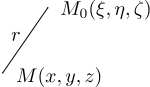
\includegraphics{figPotentialTheo1.pdf}
\end{wrapfigure}
Пусть в некоторой точке $M_0(\xi, \eta, \zeta)$ помещена масса $M$. По закону всемирного тяготения на массу $m$, помещённую в точке $M(x, y, z)$, действует сила притяжения
\[
	F = - \gamma \frac{mM}{R^2} r
\]
где $r = \frac{1}{R}$ --- единичный вектор в направлении $\overrightarrow{M_0M}$, а $\gamma$ --- гравитационная постоянная. 
Сила называется потенциальной, если существует функция, через которую она выражается как градиент некоторой потенциальной фукнции:
\[
	F = \mathrm{grad} \Pi
\]
Покажем, что при $\gamma M = 1$ сила выражается так
\[
	F = \mathrm{grad} \left(\frac{m}{r} \right)
\]
Силовое поле описывается потенциалом $\frac{m}{r}$. Если будет $n$ точек, то $\sum\limits_{i=1}^n \frac{M_i}{r_i}$. \\
Если масса распределена непрерывно, то 
\[
	\iiint\limits_{\omega} \frac{\rho (\xi, \eta, \zeta)}{\sqrt{(x - \xi)^2 + (y - \eta)^2 + (z - \zeta)^2}}\, d\omega
\]

В дальнейшем $\rho$ мы будем называть плотностью потенциала. Плотность может распределяться не только по объёму, но и по поверхности. Помимо объёмного потенциала будем рассматривать поверхностный потенциал:
\[
	\iint\limits_S \frac{\nu(\xi, \eta, \zeta)}{r}\, dS;
\]
\[
	\iint\limits_S \mu (\xi, \eta, \zeta) \derp{}{\vec n}{} \frac{1}{R}\, dS.
\]
где $\nu, \mu$ --- плотности.
Особая точка $(\xi, \eta, \zeta)$. Тогда $\Omega = \omega_1 + \omega_2$.\\
\[
	V_1 = \iiint\limits_{\omega_1} \quad V_2 = \iiint\limits_{\omega_2}
\]
Рассмотрим объём $V_2$:
\begin{multline*}
	\derp{V_2}{x}{2} + \derp{V_2}{y}{2} + \derp{V_2}{z}{2} = \iiint\limits_{\omega_2} \rho(\xi, \eta, \zeta) \left(\derp{}{x}{2} \left(\frac{1}{r} \right)  \right)  + \derp{}{y}{2} \left(\derp{}{x}{2} \left(\frac{1}{r} \right) \right)  +  \derp{}{z}{2} \left(\derp{}{x}{2} \left(\frac{1}{r} \right) \right) d\omega_2 = 0
\end{multline*}
Теперь рассмотрим $V_1$:
\[
	\derp{V}{x}{} = \iiint\limits_{\omega_1} \rho_0 (\xi, \eta, \zeta) \derp{}{x}{} \left(\frac{1}{r} \right)\, d \omega_1
\]
Аналогично по $y$ и по $z$:
\[
	\derp{}{x}{} \left(\frac{1}{r} \right) = - \frac{1}{r^2} \derp{r}{x}{} = - \frac{1}{r^3} (x \xi) = - \derp{}{\xi}{} \left(\frac{1}{r} \right)
\]
Функция $\rho$ --- непрерывная по $\Omega$.
\begin{multline*}
	 \derp{V}{x}{} = - \iiint\limits_{\omega_1} \rho (\xi, \eta, \zeta) \derp{}{\xi}{} \left(\frac{1}{r} \right)\, d\omega_1 = - \iiint\limits_{\omega_1} \left[\derp{}{\xi}{} \left(\rho \frac{1}{r} \right) - \frac{1}{r} \derp{\rho}{\xi}{}\right]\, d\omega_1 = \\
	 - \iiint\limits_{\omega_1} \derp{}{\xi}{} \left(\frac{\rho}{r} \right)\, d\omega_1 + \derp{\rho_{\text{сред}}}{\xi}{}  \int\limits_0^{2\pi} d \varphi \int\limits_0^{ \pi} d\theta \frac{1}{\varepsilon} \varepsilon^2 \sin \theta =
\end{multline*}

\begin{wrapfigure}{l}{0.2\textwidth}
	\centering
	\includegraphics{figPotentialTheo2.pdf}
\end{wrapfigure}
$\varepsilon$ --- радиус малой сферы $\omega_1 \to 0$. Применим теорему Остроградского--Гаусса и перейдём к интегралу по поверхности:
\[
	 = - \iint\limits_{s_1} \frac{\rho}{r} \cos d S_1
\]
$\alpha$ --- угол между $n$ и $x$.


\begin{align*}
	&\derp{V}{x}{2} = - \iint\limits_{s_1} \rho(\xi, \eta, \zeta) \cos \alpha \derp{}{x}{} \left(\frac{1}{r} \right) dS_1 = \iint\limits_{S_1} \frac{\rho(\xi, \eta, \zeta) \cos \alpha}{r^2} \cos \theta dS_1 = - \iint\limits_{S_1} \frac{\rho(\xi, \eta, \zeta) \cos^2 \alpha}{r^2}\, dS_1\\
	&\derp{V}{y}{2} = - \iint\limits_{S_1} \frac{\rho(\xi, \eta, \zeta) \cos^2 \beta}{r^2}\, dS_1\\
	&\derp{V}{z}{2} = - \iint\limits_{S_1} \frac{\rho(\xi, \eta, \zeta) \cos^2 \gamma}{r^2}\, dS_1
\end{align*}



\[
	\delta V = \derp{V}{x}{2} + \derp{V}{y}{2} + \derp{V}{z}{2} = - \iint\limits_{S_1} \frac{\rho(\xi, \eta, \zeta)}{r^2} (\cos^2 \alpha + \cos^2 \beta + \cos^2 \gamma) dS_1 =  - \iint\limits_{S_1} \frac{\rho(\xi, \eta, \zeta)}{r^2}\, dS_1 
\]
Воспользуемся теоремой о среднем:
\[
	 - \iint\limits_{S_1} \frac{\rho(\xi, \eta, \zeta)}{r^2} dS_1 = - \rho_{\text{ср}}(\xi, \eta, \zeta) \int\limits_0^{2 \pi} \int\limits_0^{\pi} \frac{1}{\varepsilon^2} \sin \theta \varepsilon^2\, d \theta = - 4 \pi \rho(\xi, \eta, \zeta)
\]
Обозначим $\rho = \frac{f}{4 \pi}$ и поулчим:
\[
	\Delta V = \Delta V_2 + \Delta V_2 = - f
\]
Объёмный потенциал является решением неоднородного уравнения Лапласа.
\[
	V= \frac{1}{4 \pi} \iiint\limits_{\omega} \frac{f(\xi, \eta, \zeta)}{r} d\Omega
\]
Теперь рассмотрим поверхностный интеграл.\\
Потенциал простого слоя:
\[
	\iint\limits_S \mu(\xi, \eta) \frac{1}{r}\, dS
\]
Потенциал двойного слоя:
\[
	\iint\limits_S \nu (\xi, \nu) \derp{}{n}{} \left(\frac{1}{r} \right)\, dS
\]\\


Вспомним формулу Грина:
\[
	\iint\limits_S \left(u\derp{G}{n}{} - G \derp{u}{n}{}  \right) d S - \iiint\limits_\omega (u \Delta G - G \Delta u) d\Omega = \begin{cases}
		4 \pi u &\mbox{внутри}\\
		2 \pi u &\mbox{на границе}\\
		0 &\mbox{снаружи}
	\end{cases}.
\]
Пусть $G = \frac{1}{r}$ в качестве возьмём $u = \nu_0$
\[
	\Delta \nu_0 = 0 \qquad \derp{\nu_0}{n}{} = 0
\]
\[
	\nu_0 = - \frac{1}{4 \pi} \iint\limits_{\nu_0} \derp{}{n}{} \left(\frac{1}{r} \right)\, dS
\]
\[
	\iint\limits_S \left(\nu_0 \derp{}{n}{} \left(\frac{1}{r} \right) \right)\, dS = \begin{cases}
		4 \pi \nu_0 \\
		2 \pi \nu_0 \\
		0 
	\end{cases}
\]
\[
	W_{\text{в}}^0 = - \frac{1}{4 \pi} \iint\limits_S \nu_0 \derp{}{n}{} \left( \frac{}{n} \right)\, dS
\]
\[
	W_{\text{ср}}^0 = - \frac{1}{2 \pi} \iint\limits_S \nu_0 \left(\frac{1}{r} \right)\, dS
\]
\[
	W_{\text{н}}^0 = 0
\]\\

\[
	W_{\text{в}}^0 = W_0 + 2 \pi \nu_0
\]
\[
	W_{\text{н}}^0 = W_0 - 2 \pi \nu_0
\]
При переходе через границу потенциал двойного слоя терпит разрыв
\[
	I = \iint\limits_S (\nu - \nu_0) \derp{}{n}{} \left(\frac{1}{r} \right) dS = \iint\limits_{S_1} (\nu - \nu_0) \derp{}{n}{} \left(\frac{1}{r} \right) dS + \iint\limits_{S-S_1} (\nu - \nu_0) \derp{}{n}{} \left(\frac{1}{r} \right) dS
\]
\[
	 \iint\limits_S (\nu - \nu_0) \derp{}{n}{} \left(\frac{1}{r} \right) dS \leqslant \varepsilon \iint\limits_{S_1} \derp{}{n}{} \left(\frac{1}{r} \right)\, dS 
\]
\[
	\varepsilon \iint\limits_{S_1} \derp{}{n}{} \left(\frac{1}{r} \right)\, dS = - \varepsilon \iint\limits_{S_1} \frac{\cos \alpha}{r^2}\, dS = - \varepsilon \int\limits_0^{2 \pi} d\varphi \int\limits_0^\pi \sin \theta\, d\theta
\]
\begin{multline*}
	W_{\text{в}} = \iint\limits_S \left[\nu \derp{}{n}{} \frac{1}{r} - \nu_0 \derp{}{n}{} \frac{1}{r} + \nu_0 \derp{}{n}{} \frac{1}{r} \right] dS =
\iint\limits_S \nu_0 \derp{}{n}{} \frac{1}{r} dS = I + W_{\text{в}}^0 = \underbrace{I + W_0(\nu_0)}_{W_0(\nu)} - 2 \pi \nu_0
\end{multline*}

\[
	W_{\text{в}} = W_0(\nu) - 2 \pi \nu
\]
\[
	W_{\text{н}} = W_0(\nu) + 2 \pi \nu
\]
\[
	W_{\text{в}}(M)  = \iint\limits_S \nu \derp{}{n}{} \frac{1}{r} - 2 \pi \nu \big|_S
\]
\[
	\Delta W = 0 \quad W = - \iint\limits_S \nu(\xi, \eta) \derp{}{n}{} \frac{1}{r} dS
\]
на границе  $W|_S = f$\\
\[
	W_{\text{в}} = \iint\limits_S \nu \derp{}{n}{} \frac{1}{r} - 2 \pi \nu = f
\]

\begin{equation}
	\nu(P_0) - \frac{1}{2 \pi} \iint\limits_S \nu(P) \derp{}{n}{} \frac{1}{r} dS = - \frac{1}{2 \pi} f (P_0)
	\label{equ:equUnique1}
\end{equation}
Уравнение \eqref{equ:equUnique1} является уравнением Фредгольма 2-го рода.

Из него можем определить плотности поверхностного потенциала $\nu$
\[
	W_{\text{в}} = \oint \nu \derp{}{n}{} \left(\ln \frac{1}{r} \right) dl
\]
\[
	\nu(P_0) - \frac{1}{\pi} \oint \nu (P) \derp{}{n}{} \left(\ln \frac{1}{r} \right) dl = - \frac{1}{\pi} f (P_0)
\]
\[
	W_{\text{в}} - \oint \nu \derp{}{n}{} \left(\ln \frac{1}{r} \right)
\]
На границе должно выполняться:
\[
	\nu (p_0) - \frac{1}{\pi} \oint \nu(p) \derp{}{n}{} \left(\ln \frac{1}{r} \right)\, dl = - \frac{1}{\pi} f(p_0)
\]
 \newpage

	\subsubsection{Примеры краевых задач}
		\begin{example}{Первая краевая задача для круга.}
Уравнение Фредгольма можно переписать\\
\[
	\nu(S_0) - \frac{1}{\pi} \oint \nu (S) \derp{}{n}{} \left(\ln \frac{1}{r} \right) dS = - \frac{1}{\pi} f(S_0)
\]
\[
	\derp{}{n}{} = - \derp{}{r}{}
\]
\[
	\nu (S_0) - \frac{1}{\pi} \oint \nu(S) \frac{\cos \varphi}{r} dS = - \frac{1}{\pi} f(S_0)
\]
\[
	\cos \varphi = \frac{r}{2 R}
\]
\[
	\nu (S_0) - \frac{1}{\pi} \oint \frac{\nu(S)}{2 R} dS = - \frac{1}{\pi} f(S_0)
\]
\[
	\nu (S) = - \frac{1}{\pi} f (S) + A
\]
\[
	- \frac{1}{\pi} \cancel{f(S_0)} + A - \frac{1}{2 R \pi} \oint \left(A - \frac{1}{\pi} f(S) \right) dS = - \frac{1}{\pi} \cancel{f(S_0)}
\]

\[
	- \oint_G \nu(p) \derp{}{n}{} \left(\ln \frac{1}{r} \right) d \gamma + \pi \nu (P_0) = f (P_0)
\]
\[
	\oint_G \nu(P) \frac{\cos \varphi}{r} d \gamma + \pi \nu (P_0) = f (P_0)
\]
\[
	\oint_G \nu(p) \derp{\gamma}{2R}{} + \pi \nu (P_0) = f(P_0)
\]
\[
	\pi \nu(P_0) + \int\limits_0^{2 \pi} \nu (\theta) \frac{d \theta}{2} = f (P_0)
\]

\[
	\oint_G \frac{\nu(S)}{2 R} dS + \pi \nu(S_0) = f(S_0)
\]
\[
	\nu(S) = \frac{f(S)}{\pi} + A
\]
\[
	\oint_G \frac{A + \frac{f(s)}{\pi}}{2R} dS +  \pi (A + \frac{\cancel f(S_0)}{\pi}) = \cancel f(S_0)
\]
\[
	\oint_G \frac{A}{2 P} dS + \oint_G \frac{f(S)}{2 \pi R} dS + \pi A = 0
\]
Итак, у нас получилось такое уравнение\\
\[
	\frac{A}{2R}\oint dS + \oint_G \frac{f(\xi) d\xi}{2 \pi R} + \pi A = 0
\]
\[
	\frac{A \cdot 2 \pi R}{2 R} + \oint_G \frac{f(\xi) d\xi}{2 \pi R} + \pi A = 0
\]

\[
	\nu(S) = \frac{1}{4 \pi^2 R} \oint f(\xi) d \xi + \frac{f(S)}{\pi}
\]


\[
	u(M) = - \oint_G \left[\frac{f(S)}{\pi} - \frac{1}{4 \pi^2 R} \oint f(\xi) d\xi \right] \frac{1}{r} \cos \varphi dS
\]
\[
	\cos \varphi = \frac{r}{R}
\]
\begin{multline*}
	 = \oint_G \frac{f(S)}{\pi} \frac{\cos \varphi}{r} dS - \frac{1}{4 \pi^2 R} \oint_G f(\xi) d \xi \oint_G \frac{\cos \varphi}{r} dS =\\ 
	 = \oint_G \left(\frac{f(S)}{\pi} \frac{\cos \varphi}{r} - \frac{1}{2 \pi^2 R} f(S) \right) dS = \frac{1}{\pi} \oint f(S) \left[\frac{\cos \varphi}{r} - \frac{1}{2 R} \right]dS
\end{multline*}
\[
	r^2 = R^2 + \rho_0^2 - 2 R \rho_0 \cos(\theta - \theta_0) \frac{\cos \varphi}{r} dS - \frac{1}{4 \pi^2 R}
\]
\[
	u(\theta) = \frac{1}{2 \pi } \oint \frac{f(\theta) (R^2 - \rho_0^2) d\theta}{(R^2 \rho_0^2 - 2 R \rho_0 \cos(\theta - \theta_0))}
\]
\end{example}

\begin{example}{Первая краевая задача для полупространства.}
Найти гармоническую функцию, непрерывную всюду в области $z \geqslant 0$, принмающую на границе $z = 0$ заданное значение $f(x, y)$.

\[
	W(x, y, z) = - \iint\limits_S \nu (P) \derp{}{n}{} \left(\frac{1}{r} \right)\, dS
\]
\[
	r = \sqrt{(x - \xi)^2 + (y - \eta)^2 + (z - \theta)^2}
\]
\[
	-\frac{1}{2\pi} \iint\limits_S \nu(P) \derp{}{n}{} \left(\frac{1}{r}\right) dS + \nu (P_0) = f(P_0)
\]
\[
	\frac{1}{2 \pi} \iint\limits_S \nu(P) \frac{\cos \varphi}{r^2} dS + \nu (P_0) = \frac{1}{2 \pi} f(P_0)
\]
\[
	\cos \varphi = \derp{r}{z}{} = \frac{2 z}{2 \sqrt{(x - \xi)^2 + (y - \eta)^2 + (z - \theta)^2}} = \frac{z}{r}
\]
\[
	z = 0 \quad \cos \varphi = 0
\]
\[
	\nu(P) = \frac{1}{2 \pi} f(P)
\]
\[
	u = \frac{1}{2 \pi} \iint\limits_S f(P) \frac{1}{r^2} \derp{r}{z}{} dS = \frac{1}{2 \pi} \iint\limits_S f(P) \frac{z}{r^3} dS
\]
\[
	u(x, y, z) = \frac{1}{2 \pi} \int\limits_{-\infty}^{\infty}\int\limits_{-\infty}^{\infty} f(\xi, \eta) \frac{z}{[(x - \xi)^2 + (y - \eta)^2 + z^2]^{\frac{3}{2}}} d \xi d \eta
\]
\end{example}
Вторая задача (задача Неймана) находится в виде потенциала простого слоя.
Потенциал простого слоя удовлетворяет уравнению Лапласа. Осталось удовлетворить краевым условиям.
\[
	\derp{u}{n}{} = \iint\limits_S \mu(\xi, \eta, \zeta) \derp{}{n}{} \left(\frac{1}{r} \right) dS
\]
\[
	- \iint\limits_S \mu \derp{}{n}{} \left(\frac{1}{r} \right) dS + 2 \pi \mu(P_0) - f(P_0) = 0
\]
\[
	\iint\limits_S \mu \derp{}{n}{} \left(\frac{1}{r} \right) dS - 2 \pi \mu (P_0) = - f(P_0)
\]
\[
	- \iint\limits_S \mu (P) \derp{}{n}{} \left(\frac{1}{r} \right) dS = - f
\]
\[
	\iint\limits_S \mu (P) \derp{}{n}{} \left(\frac{1}{r} \right) dS + 2 \pi \mu (P_0) = -f 
\]
\[
	\mu(P_0) - \frac{1}{2 \pi} \iint\limits_S \mu(P) \derp{}{n}{} dS = - \frac{1}{2 \pi} f
\]






 \newpage

	%\subsection{Пример пример}
		%Рассмотрим задачу 
\[ \derp{u}{x}{2} + \derp{u}{y}{2} = -1 \]

\[ \abs{x} \leq 1 \]
\[ \abs{y} \leq 1 \]

\[ I[u(x, y)] = \iint\limits_D \left\{ \left(\derp{u}{x}{} \right)^2 + \left(\derp{u}{y}{} \right)^2 - 2 u \right\}\, dx dy \]

из метода фурье для уравнения теплопроводности
\[u(x, t) = \sum C_n e^{- \left( \frac{\pi n}{l} a\right)^2 t} \sin \frac{\pi n}{l} x\]
	\[C_n = \frac{2}{l} \int\limits_{0}^{1} f (\xi) \sin \frac{\pi n}{l} \xi d \xi \leqslant \frac{2}{l} k \quad \abs{f(x)} < k\]
	\[\derp{u}{t}{} = - \sum C_n \left( \frac{\pi n}{l} a\right)^2 e^{- \left( \frac{\pi n}{l} a\right)^2 t} \sin \frac{\pi n}{l} x\]
	\[\derp{u}{x}{2} = - \sum C_n \left( \frac{\pi n}{l} a\right)^2 e^{- \left( \frac{\pi n}{l} a\right)^2 t} \sin \frac{\pi n}{l} x\] \newpage
	%\subsection{Приближённые методы расчета колебаний}
		%Возникает необходимость в способах, позволяющих достаточно просто рассчитывать и сложные системы.

Один из возможных путей состоит в применении простых приближенных формул (например, формулы Рэлея). В этом случае задают форму колебаний системы, сводя её таким образом к системе с одной степенью свободы. При удачной аппроксимации получают достаточно точное значение низшей собственной частоты системы, однако другие её динамические характеристики остаются нераскрытыми.

Cхематизация реальной системы, как имеющей несколько степеней свободы, достигается в методе Рэлея-Ритца, при использовании которого форма колебаний системы задаётся в виде выражения, включающего несколько параметров.

Другим приёмом, позволяющим свести реальную систему к системе с конечным числом степеней свободы, является метод прямой дискредитации. Чем больше число элементов, на которые разбита система при использовании этого метода, тем ближе расчётная схема к исходной системе. Вместе с тем, если элементы выбраны однотипными, то даже при большом их числе оказывается возможным реализовать расчёт колебаний, используя матричные методы с применением ЭВМ. Примерами таких методов являются метод начальных параметров в форме матриц перехода и метод прогонки.

При динамических расчётах конструкций сложной конфигурации также широко используется метод конечных элементов.

В том случае, когда сложную колебательную систему можно разделить на несколько подсистем, динамические характеристики которых определяются сравнительно просто, полезными являются методы динамических податливостей и жёсткостей. Эти методы представляют собой обобщение на динамические задачи метода сил и метода перемещений строительной механики.

В методе последовательных приближений задача об определении собственных частот и форм колебаний сводится к многократному расчёту деформаций системы под действием известной статической нагрузки.
\section{Применение вариационных методов в решение задач математической физики}
		%Предположим,что исходная кривая $y = f(x)$. И мы данную кривую проварьируем, то есть рассмотрим множество кривых. Данное множество можно описать одним уравнением -- $\tilde y (x, \alpha) = y(x) + \alpha \eta (x)$, где $\eta \in C_1 \quad \eta(a) = \eta(b) = 0$. $\eta$ может принимать любой знак. Необходимо рассмотреть функционал на параметрическом семействе кривых.
\[
	I(\tilde y(x, \alpha)) = \int\limits_a^b F(x, \tilde y (x, \alpha), \tilde y' (x, \alpha)\, dx
\]
После взятия интеграла получаем
\[
	I[\tilde (x, \alpha)] = \tilde I( \alpha)
\]
а необходимое условие экстремума функционала записывается так
\begin{equation} \delta I = \lim\limits_{\alpha \to 0} \derp{\tilde I}{\alpha}{} = 0 \label{}\end{equation}
такой предел называется \textit{первой вариацией функционала}.
Продифференциировали $I$ по $\alpha$\\
\[
	\derp{\tilde I}{\alpha}{} = \int\limits_a^b \left(\derp{F}{\tilde y}{}  \eta (x) + \derp{F}{y'}{} \eta'(x) \right) dx = 0
\]
Вспомним свойство интегралов. Первое слагаемое оставим без изменений, а второе возьмём по частям.
\[
	\int\limits_a^b \derp{F}{y}{} \eta(x) dx + \derp{F}{y'}{} \eta(x) |_a^b - \int\limits_a^b \derp{F}{y'}{} \eta (x) dx = 0
\]
Таким образом на концах отрезком функция обращается в 0.
В итоге
\[
	\delta I = \int\limits_a^b \left(\derp{F}{y}{} - \der{}{y'}{} \derp{F}{x}{} \right)
\]
В силу произвольности $\eta(x)$ окончательное необходимое условие записывается в виде уравнения Эйлера. 
\[
	\der{}{x}{} \derp{F}{y'}{} - \derp{F}{y}{} = 0
\]
\subsection{Вариационные задачи с кратными интегралами.}

Функция $\varphi$ определена на области.
\begin{multline*}
	I(\varphi(x, y)) = \iint\limits_D F(x, y, \varphi(x, y), \derp{\varphi}{x}{}, \derp{\varphi}{y}{})\, dx dy + \int\limits_\gamma G(\varphi (x, y), \varphi' (x, y)) d \gamma =\\= \iint\limits_D \left( \left(\derp{\varphi}{x}{} \right)^2 + \left(\derp{\varphi}{y}{} \right)^2 - c \varphi^2 - 2 f \varphi \right)\, dx dy + \int\limits_\gamma ((\delta \varphi^2 - c \varphi))
\end{multline*}
Множество поверхностей, все выходят из $\gamma$.

\begin{multline*}
	I [ \tilde \varphi (x, y)] = \iint\limits_D \left\{ \left[ \derp{}{x}{} (\varphi + \alpha \eta)\right]^2 + \left[ \derp{}{y}{} (\varphi + \alpha \eta)\right]^2 - C [\varphi + \alpha \eta]^2 + 2 f (\varphi + \alpha \eta)\right\}\, dx dy +\\+ \int\limits_\gamma \left[ \delta (\varphi + \alpha \eta) - c c (\varphi + \alpha \eta)\right] d \gamma 
\end{multline*}

\[
	 \derp{I}{\alpha}{} = \iint\limits_D \left\{ 2 \left[ \derp{\varphi}{x}{} + \alpha \derp{\eta}{x}{}\right] \derp{\eta}{x}{} + 2 ? \right\}\, dx dy 
\]

\[
	 \delta I \lim\limits_{\alpha \to 0} \derp{\tilde I}{\alpha}{} = 2 \iint\limits_D \left\{ \derp{\psi}{x}{} \derp{\eta}{x}{} + \derp{\varphi}{y}{} \derp{\eta}{y}{} - c \varphi \eta - f \eta \right\} + \int\limits_\gamma (2 \delta \varphi \eta - c \eta)\, d \gamma = 0 
\]
\[
	\delta I = 2 \iint\limits_D \left\{ \derp{}{x}{} \left[ \derp{\varphi}{x}{} \eta \right] \derp{\varphi}{x}{2} \eta + \derp{}{y}{} \left(\derp{\varphi}{y}{} \eta \right) - \derp{\varphi}{y}{2} \eta - c \varphi \eta - f \eta \right\}\, dx dy + \int\limits_\gamma [ 2 \delta [ \xi \eta - c \eta], d \gamma 
\]

%\[
%	 2 \iint\limits_D \left\{ \derp{}{x}{} \left[ \derp{\varphi}{x}{} \eta\right] - \right\}
%\]

Первая вариация должна быть равна 0 в силу первого условия экстремума.

\begin{align}
   \derp{\varphi}{x}{2} + \derp{\varphi}{y}{2} + c \varphi + f = 0\\
   \derp{\varphi}{n}{} \delta \varphi - \frac{c}{2} = 0 |_\gamma
\end{align}

Третья краевая задача для эллиптического уравнения.

Решить задачу и минимизировать функционал - две эквивалентные задачи.
На практике как правило краевые задачи аналитически не решаются, а применяются численные методы, так как минимизировать функционал проще.
	\subsection{Вариационная формулировка краевых задач}\label{que:35}
			Введём понятие функционала. $y = f(x)$ --- отображение числового множества $r \in X$ на числовое множество $y \in Y$ --- функция. $X$ --- конечномерное множество
\begin{equation}
	\mathrm{I} [y(x)] = \int\limits_a^b F(x, y(x), y'(x))\,dx
	\label{equ:Variz1}
\end{equation}
Функционал \eqref{equ:Variz1} отображает множество функций на числовое множество. Множество функций является областью определения.\\

\textbf{Задача Бернулли}\\
\begin{figure}[h!]
	\centering
	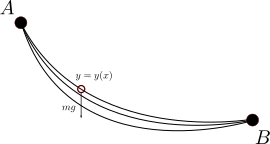
\includegraphics{figVariaz.pdf}
\end{figure}

Требуется найти кривую $y(x)$, чтобы шарик попал из ($\cdot$)$A$ в ($\cdot$)$B$ c наименьшей скоростью
\[
	t = \int\limits_a^b  \frac{\sqrt{1 + y'^2}}{\sqrt{2 g y}}\, dx
\]

Найдо найти экстремум функционала $\mathrm{I}[y(x)]$ на множестве непрерывно дифференциируемых функций: $y(x) \in C_1$.
Предположим, что искомая кривая --- прямая, соединяющая $A$ и $B$
\begin{wrapfigure}{r}{0.4\textwidth}
	\centering
	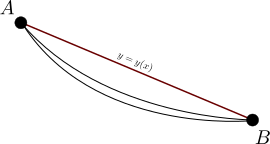
\includegraphics[width=0.4\textwidth]{figVariaz2.pdf}
\end{wrapfigure}
Рассмотрим множество кривых. Их можно описать уравнением
\[
	\tilde y (x, \alpha) = y (x) + \alpha\eta(x), \quad 0 \leqslant \alpha \leqslant 1.
\]
\[
	\eta \in C_1 \qquad \eta(a) = \eta(B) = 0
\]
Необходимо рассмотреть функционал на однопараметрическом семействе кривых:
\[
	\mathrm{I}[\tilde y (x, \alpha)] = \int\limits_a^b F(x, \tilde y(x, \alpha), \tilde y'(x, \alpha)) \, dx
\]
Искомая кривая будет получаться при $\alpha = 0$. Предположим нам удалось взять интеграл в аналитическом виде, когда $x$ у нас пропадает и получаем функцию зависящую только от $\alpha$:
\[
	\tilde{\mathrm{I}}(\alpha)
\]
Необходимое условие экстремума функционала:
\[
	\delta \mathrm{I} = \lim\limits_{\alpha \to 0} \derp{\tilde{\mathrm{I}}}{\alpha}{} = 0 
\]
--- \textit{первая вариации функционала}.
\[
	\derp{\tilde{\mathrm{I}}}{\alpha}{} = \int\limits_a^b \left(\derp{F}{\tilde y}{} \derp{\tilde y}{\alpha}{} + \derp{F}{\tilde y}{} \derp{\tilde y'}{\alpha}{} \right)\, dx
\]
\[
	\derp{\tilde y}{\alpha}{} = \eta (x) \qquad \derp{\tilde y '}{\alpha}{} = \eta' (x)
\]
Таким образом 
\[
	\derp{\tilde{\mathrm{I}}}{\alpha}{} = \int\limits_a^b \left(\derp{F}{\tilde y}{} \eta (x) + \derp{F}{\tilde y}{} \eta'(x)\right)\, dx.
\]
Переходим к пределу, чтобы получить первую вариацию:
\[
	\delta \mathrm{I} \lim\limits_{\alpha \to 0} \derp{\tilde{\mathrm{I}}}{\alpha}{} = \int\limits_a^b \left(\derp{F}{y}{} \eta(x) + \derp{F}{y}{} \eta'(x)\right)\, = 0
\]
\[
	\int\limits_a^b \derp{F}{y}{} \eta(x)\, dx + \derp{F}{y'}{} \eta(x) \Big|_a^b - \int\limits_a^b \der{}{x}{} \derp{F}{y'}{} \eta(x)\, dx = 0
\]
На концах отрезка произвольная функция обращается в 0.
\[
	\delta I = \int\limits_a^b \left(\derp{F}{y}{} - \der{}{x}{} \derp{F}{y'}{} \right) \eta(x)\, dx = 0
\]
Так как $\eta(x)$ --- произвольная, то $\int = 0$ только в случае, когда выражение в скобках $= 0$\\

Окончательное условие для функционала записывается в виде уравнения Эйлера:
\[
	\der{}{x}{} \derp{F}{y'}{} - \derp{F}{y}{} = 0
\]


\subsubsection{Вариационная задача с кратным интегралом.}
Возьмём на плоскости $xOy$ область $D$ и на ней построим цилиндр, покрытый поверхностью $z = \varphi(x, y)$:
\begin{wrapfigure}[3]{l}{0.35\textwidth}
	\centering
	\includegraphics[width=0.35\textwidth]{figVariaz3.pdf}
\end{wrapfigure}
\begin{align*}
	&\mathrm{I} [\varphi(x, y)] = \iint\limits_S F(x, y, \varphi(x, y), \derp{\varphi}{x}{}, \derp{\varphi}{y}{})\, dx dy +{} \\
	&\phantom{\mathrm{I} [\varphi(x, y)]=} + \int\limits_\gamma G(\varphi(x, y), \varphi'(x, y))\, d\gamma =\\
	&\phantom{\mathrm{I} [\varphi(x, y)]} = \int\limits_D \left(\left(\derp{\varphi}{x}{} \right)^2 + \left(\derp{\varphi}{y}{} \right)^2 - c \varphi^2 - 2 f \varphi\right)\, dx dy + {}\\
	&\phantom{\mathrm{I} [\varphi(x, y)]=} + \int\limits_\gamma \left(\sigma \varphi^2 - c \varphi \right)\, d \gamma
\end{align*}\\

Мы должны рассмотреть однопараметрическое семейство плоскостей:
\[
	\tilde \varphi(x, y) = \varphi (x ,y) + \alpha \eta (x, y),
\]
выходящих из контура $\gamma$: $r \big|_\gamma = 0$


\begin{multline*}
	\mathrm{I} [\tilde \varphi(x, y)] = \iint\limits_S \left\{\left[ \derp{}{x}{} (\varphi + \alpha r) \right]^2 + \left[\varphi + \alpha r \right]^2  - c [\varphi + \alpha r]^2 - 2 f (\varphi + \alpha r)\right\}\, dx dy  +{}
	\\+ \int\limits_\gamma \left[ \sigma (\varphi + \alpha r)^2 - c (\varphi + \alpha r) \right]\, d\gamma = \\
	= \iint\limits_S \left\{\left(\derp{\varphi}{x}{} + \alpha \derp{r}{x}{} \right)^2 + \left(\derp{\varphi}{y}{} + \alpha \derp{r}{y}{}\right) - c (\varphi + \alpha r)^2 - 2 f (\varphi + \alpha r)\right\}\, dx dy +{}
	\\+ \int\limits_\gamma \left[\sigma (\varphi + \alpha r)^2 - c (\varphi + \alpha r) \right]\, d\gamma
\end{multline*}
\begin{multline*}
	\derp{I}{\alpha}{} \iint\limits_D \left\{ 2 \left[\derp{\varphi}{x}{} + \alpha \derp{r}{x}{} \right] \derp{r}{x}{} + 2 \left(\derp{\varphi}{y}{} + \alpha \derp{r}{y}{} \right) \derp{r}{y}{}  - 2 c (\varphi + \alpha r) r - 2 f r \right\}\, dx dy +{}\\
	+ \int\limits_\gamma \left\{2 \left[\sigma \left(\varphi + \alpha r \right)r \right] - c r\right\}\, d \gamma
\end{multline*}
\[
	\delta \mathrm{I} = \lim\limits_{\alpha \to 0} \derp{\tilde{\mathrm{I}}}{\alpha}{} = 2 \iint\limits_D \left\{ \derp{\varphi}{x}{} \derp{r}{x}{} + \derp{\varphi}{y}{} \derp{r}{y}{} - c \varphi - f r \right\}\, dx dt + \int\limits_\gamma (2 \sigma \varphi r - c r)\, d \gamma = 0
\]
\[
	\delta \mathrm{I} = 2 \iint\limits_D \left\{\derp{}{x}{} \left[\derp{\varphi}{x}{} r \right] - \derp{\varphi}{x}{2} r + \derp{}{y}{} \left(\derp{\varphi}{y}{} r \right) - \derp{\varphi}{y}{2} r - c \varphi r - f r\right\}\, dx dy =
	\int\limits_\gamma \left[ w \sigma \varphi r - c r \right]\, d\gamma
\]
\begin{multline*}
	\iint\limits_D \left[\derp{}{x}{} \left( \derp{\varphi}{x}{} r \right) + \derp{}{y}{} \left( \derp{\varphi}{y}{} \right) r \right]\, dx dy 
	= \int\limits_\gamma \left[ \derp{\varphi}{x}{} r \cos (n x) + \left(\derp{\varphi}{y}{} r \right) \cos (n y) \right]\, d\gamma=\\
	= \int\limits_\gamma \overrightarrow{\mathrm{grad} \varphi} \vec n r\, d\gamma = \int\limits_\gamma \derp{\varphi}{n}{} r\, d\gamma
\end{multline*}
\[
	\delta \mathrm{I} = 2 \iint\limits_D \left[- \left(\derp{\varphi}{x}{} + \derp{\varphi}{y}{2}\right) - c \varphi - f \right] r \, dx dy + \int\limits_\gamma (2 \sigma \varphi - c + 2 \derp{\varphi}{n}{}) r \, d\gamma = 0
\]

\subsubsection{Вариационная формулировка задач}
Третья краевая задача для уравнения эллиптического типа:
\[
	\begin{cases}
		\displaystyle\derp{\varphi}{x}{2} + \derp{\varphi}{y}{} + c \varphi - f = 0\\
		\displaystyle\derp{\varphi}{n}{} + \sigma \varphi - \frac{c}{2} = 0 \Big|_\Gamma
	\end{cases}
\]
Решить краевую задачу и минимизировать функционал
\[
	\mathrm{I} [\varphi(x, y)] = \iint\limits_D \left\{\left(\derp{\varphi}{x}{} \right)^2 + \left(\derp{\varphi}{y}{} \right)^2 - c \varphi^2 - 2 f \varphi \right\}\, dx dy + \int\limits_\gamma \left(\sigma \varphi^2 - c \varphi\right)\, d\gamma
\]
\[
	\derp{u}{x}{2} + \derp{u}{y}{2} = - 1
\]
\[
	\abs{x} \leqslant 1 \qquad \abs{y} \leqslant 1
\]
\[
	u\big|_\gamma = 0
\]
Задача Дирихле для уравнения Пуассона
\[
		\mathrm{I} [\varphi(x, y)] = \iint\limits_D \left\{\left(\derp{\varphi}{x}{} \right)^2 + \left(\derp{\varphi}{y}{} \right)^2  - 2 u \right\}\, dx dy 
\]
 \newpage

	\subsection{Метод Ритца}\label{que:36}
			\setcounter{equation}{0}
Метод Ритца служит для приближенного решения вариационной задачи. \href{http://reslib.com/book/Chislennie_metodi_analiza__Priblizhenie_funkcij__differencialjnie_i_integraljnie_uravneniya/321}{Описание.} %Зададимся несколькими функциями $f_1(x) , f_2(x) ,\ldots , f_n(x)$, каждая из которых удовлетворяет геометрическим граничным условиям задачи, и образум функцию $f(x)$ как сумму
%\begin{equation}
%	f(x) = C_1 f_1(x) +C_2 f_2(x)+...+C_n f_n(x).
%	\label{equ:equRitz1}
%\end{equation}
%Если эту функцию подставить в формулу Рэлея
%\begin{equation}
%	w^2 = \frac{\int\limits_0^l E J(f'')^2\, dx}{\int\limits_0^l m f^2 \, dx},
%	\label{equ:equRitzReley}
%\end{equation}
%то результат будет зависеть от конкретного выбора коэффициентов $C_1 , C_2 , …, C_n$.

%Метод Ритца основан на простой идее: коэффициенты $C_1 , C_2 , …, C_n$ должны быть выбраны так, чтобы вычисление по \eqref{equ:equRitzReley} дало наименьшее значение для $w^2$. Из теоремы Рэлея вытекает, что такой выбор будет наилучшим (при данной системе функций $f_i$).

%Условия минимума $w^2$ имеют вид
%\[
%	\derp{}{C_i}{}  \frac{\int\limits_0^l E J(f'')^2\, dx}{\int\limits_0^l m f^2 \, dx} = 0,
%\]
%где $i = 1, 2, \ldots, n$.
%т.е.
%\[
%	\left[\derp{}{C_i}{} \int\limits_0^l E J(f'')^2\, dx\right] \left[\int\limits_0^l m f^2 \, dx \right] - \left[[\derp{}{C_i}{} \int\limits_0^l m f^2\, dx \right] \left[\int\limits_0^l E J(f'')^2 \, dx \right] = 0
%\]

%Разделив это уравнение на интеграл $\int\limits_0^l m f^2 \, dx$ и учитывая \eqref{equ:equRitzReley}, получим

%\begin{equation}
%	\derp{}{C_i}{} \int\limits_0^l \left[ EJ(f'')^2 - w^2 m f^2\right]\, dx = 0
%	\label{equ:equRitzReley2}
%\end{equation}

%Уравнения \eqref{equ:equRitzReley2} однородны и линейны относительно $C_1 , C_2 , …, C_n$ и их число равно числу членов выражения \eqref{equ:equRitz1}. Приравнивая нулю определитель, составленный из коэффициентов при $C_1 , C_2 , …, C_n$, получим частотное уравнение. Это уравнение не только дает хорошее приближение для низшей частоты, но также определяет (хотя и с меньшей точностью) значения высших частот; при этом можно будет вычислить столько частот, сколько слагаемых принято в выражении \eqref{equ:equRitz1}.

%Метод Ритца, как и метод Рэлея, позволяет решить задачу в случаях разрывных функций $EJ$ и $m$ и когда эти функции представлены различными аналитическими выражениями на различных участках.\\

%Иногда та же идея используется в иной форме. Например, при исследовании поперечных колебаний турбинных лопаток задаются функцией $f(x) = ax^s$ (начало координат в закрепленном конце). Применяя затем формулу Рэлея \eqref{equ:equRitzReley}, получают частоту в виде зависимости от показателя степени $s$. Затем при помощи числовых расчетов определяют значение $s$, которому отвечает наименьшая частота. Это позволяет достаточно надежно определить как форму, так и частоту колебаний первого тона.\\

\begin{example}{Найти решение с помощью метода Ритца}
Подобрать полную систему линейно независимых функций $\varphi_1(x, y), \varphi_2(x, y), \ldots \varphi_n(x, y)$, удовлетворяющих граничному условию $\varphi_i|_\gamma = 0$ (все функции на граниче должны быть равны $0$).

Чаще всего это тригонометрические или степенные функции. В нашем случае удобнее выбрать степенные: 
\begin{align*}
	(1 - x^2)(1 - y^2) = \varphi_1\\
	(1 - x^2)(1 - y^2)x = \varphi_2
\end{align*}
Искомую функцию $u$ мы будем искать в виде ряда 
\[
	\sum\limits_{k = 1}^n C_k \varphi_k (x, y)
\]
где $C_k$ --- неизвестные константы.

\begin{multline*}
	\iint\limits_D \biggl\{ \left(\sum\limits_{k = 1}^n C_k \derp{\varphi_k}{x}{} \right)^2 + \left(\sum\limits_{k = 1}^n C_k \derp{\varphi_k}{y}{} \right)^2 - 2 \sum\limits_{k = 1}^n C_k \varphi_x(x, y) \biggl\}\, dx dy = \\
	= \iint\limits_D \left\{ \sum_{k = 1}^n \sum_{k = 1}^n C_k C_m \derp{\varphi_k}{x}{} \derp{\varphi_m}{x}{} + \sum_{k = 1}^n \sum_{k = 1}^n C_k C_m \derp{\varphi_k}{y}{} \derp{\varphi_m}{y}{} - 2 \sum\limits_{k = 1}^n C_k \varphi_k (x, y) \right\}\, dx dy
\end{multline*}
Так как сумма конечная, меняем местами знаки суммы и интеграла:
\[
	\sum_{k = 1}^n \sum_{k = 1}^n C_k C_m \left[ \iint\limits_D \underset{a_{km}}{\left(\derp{\varphi_k}{x}{} \derp{\varphi_m}{x}{} + \derp{\varphi_k}{y}{} \derp{\varphi_m}{y}{} \right)}\, dx dy \right] - 2 \sum\limits_{k = 1}^n C_k \iint\limits_D \underset{b_k}{\varphi_k (x, y)}\, dx dy
\]

В итоге получили
\[
	I[u] =  \sum_{k = 1}^n \sum_{k = 1}^n C_k C_m a_{km} - 2 \sum\limits_{k = 1}^n C_k b_k
\]
Константы $C_1, C_2, \ldots, C_n$ --- должны быть подобраны так, чтобы функционал $I [C_1, C_2, \ldots, C_n]$ принимал минимальные значения.
\[
	\derp{I}{C_1}{} = 0 \quad \derp{I}{C_2}{} = 0 \quad \derp{I}{C_n}{} = 0
\]
В результате получаем СЛАУ:

\[
	\begin{matrix}
	   a_{11} C_1 + a_{12} C_2 +\ldots +a_{1n}C_n = 2 b_1\\
	   \hdotsfor{1}\\
	   a_{n1} C_1 +a_{n2} C_2+ \ldots+ a_{nn}C_n = 2 b_n
	\end{matrix}
\]
Пусть решение состоит из 1-го слагаемого:
\[
	u(x, y) = C_1 (1 - x^2)(1 - y^2)
\]
Требуется найти $C_1$:

\begin{align*}
	&\iint\limits_D \left\{ \left[C_1 (1 - y^2)(- 2 x) \right]^2 + \left[C_1 (1 - x^2)(-2y) \right]^2 - 2 C_1 (1 - x^2)(1 - y^2) \right\}\, dx dy =\\
	&=4 C_1^2  \int\limits_{-1}^1 \int\limits_{-1}^1 \left[ x^2 (1 - y^2)^2 + y^2 (1- x^2)^2 \right]\, dx dy  - 2 C_1 \int\limits_{-1}^1 \int\limits_{-1}^1 (1 - x^2)(1 - y^2)\, dx dy =\\
	&=8 C_1^2 \int\limits_{-1}^1 \left[x^2 \left(1 - \frac{2}{3} + \frac{1}{5} \right) + \frac{1}{5} \left(1 - 2 x^2 + x^4 \right)\right]\, dx - 4 C_1 \int\limits_{-1}^1  (1 - x^2) \left(1 - \frac{1}{3}\right) \, dx =\\
	&=16 C_1^2 \left\{ \left(1 - \frac{2}{3} + \frac{1}{5} \right) \frac{x^3}{3} + \frac{1}{3} \left(x - \frac{2}{3} x^3 + \frac{1}{5} x^5 \right)\right\} \Bigg|_0^1 - 8 C_1 \left(x - \frac{x^3}{3} \right) \left(1 - \frac{1}{3}\right)\Bigg|_0^1 =\\
	&=16 C_1^2 \left\{\frac{1}{3} \frac{8}{15} + \frac{1}{3} \frac{8}{15} \right\} - 8 C_1 \left(\frac{4}{9} \right)\\
\end{align*}

\[
	\frac{16 \cdot 16}{3 \cdot 15} C_1^2 - \frac{32}{9} C_1
\]

\[
	C_1 = \frac{5}{16}
\]

\[
	u(x,y) = \frac{5}{16} (1 - x^2)(1 - y^2)
\]
Точность $1.5\%$.
\end{example}
 \newpage


\section{Распространение волн в пространстве}

	\subsection{Задача о колебании квадратной пластинки.}\label{que:14}
			Пусть в плоскости $(x, y)$ расположена прямоугольная пластинка со сторонами $a$ и $b$, закреплённая по краям и возбуждаемая с помощью начального отклонения и начальной скорости. Для нахождения функции $u(x, y, t)$ мы должны решить уравнение колебаний

	\[
		\derp{u}{t}{2} = a^2 \left(\derp{u}{x}{2} + \derp{u}{y}{2} \right)\quad x\in [0,a], y \in [0, b]
	\]
	Начальные условия при $t = 0$
	\begin{alignat*}{1}
		u&=f(x,y) \\
		\derp{u}{t}{} &= g(x,y)
	\end{alignat*}
	Граничные условия
	\begin{align*}
		x=0 \quad u=0, \quad x = a \quad u = 0\\
		y=0 \quad u=0, \quad y = b \quad u = 0\\
	\end{align*}
%\includegraphics{squareplate.pdf}

	Будем искать решение методом Фурье в виде
	\[
		u(x,y,t) = T(t) \cdot G(x,y);
	\]
	\[
	\derp{u}{t}{2} = T''  G; \qquad \derp{u}{x}{2}  = T \derp{G}{x}{2}; \qquad \derp{u}{y}{2} = T\derp{G}{y}{2}
	\]
	\[
		\left.  T''  G = a^2 T  \left(\derp{G}{x}{2} + \derp{G}{y}{2}\right) \quad \right| \frac{1}{TG}
	\]
	

	\[
		\frac{1}{a^2} \frac{T''}{T} = \frac{1}{G} \left(\derp{G}{x}{2} + \derp{G}{y}{2}\right) = - \lambda^2
	\]
		Такое равенство возможно в единственном случае\\
	\[
		T'' + a^2 \lambda^2 T = 0 \qquad \derp{G}{x}{2} + \derp{G}{y}{2} + \lambda^2 G = 0
	\]
	
	G представим в виде произведения двух функций:
	\[
		G(x,y) = X(x) \cdot Y(y)
	\]
	\[
		\frac{X''}{X} + \frac{Y''}{Y} + \lambda^2 = 0
	\]
	
	Это возможно, только если обе функции равны одной константе.
	\[
		[X = -k^2 \quad Y=-n^2]
	\]
	\[
		-k^2 -n^2 +\lambda^2 =0
	\]
	
	Таким образом получили следующие дифференциальные уравнения
	\[
		\left\{
		\begin{aligned}
			&T'' + a^2 \lambda^2 T = 0 \\
			&X'' + k^2X = 0\\	
			&Y'' + n^2 Y = 0\\
			&p^2 = k^2 + n^2\
		\end{aligned}
		\right.
	\]
	Найдём решение в виде
	\[
		u(x,y,t) = T(x) \cdot X(x)\cdot Y(y)
	\]
	\[
		x=0: u = T(t) X(0) Y(y) = 0 \Rightarrow
	\]
	\[
		X(0) = 0 \quad X(a) = 0 \quad Y(0) = 0 \quad Y(b)= 0
	\]
	Решим задачу Штурма--Лиувилля. Из граничных условий найдём $k$ и $n$:
	\begin{alignat*}{2}
		&X'' + k^2 X = 0	&\phantom{\qquad}\quad&Y'' + n^2 Y = 0\\
		&X(0) = 0 \quad X(a) = 0	&&Y(0) = 0 \quad Y(a) = 0\\
		&X(x)= C_1 \cos k x + C_2 \sin k x	&&Y(x)= C_3 \cos n x + C_4 \sin n x\\
		&C_1 = 0 \quad \sin ka= 0	&&C_3 = 0 \quad \sin ka= 0\\
		&ka = mt; \quad k = \frac{m\pi}{a} m=1,2\dots		&&n = \frac{l \pi}{b} l =1,2 \dots\\
		&X(x)= C_2 \sin  \frac{m \pi}{a} x	&&Y(y) = C_4 \sin \frac{l \pi}{b} x		
	\end{alignat*}
	Решениям уравнений соответствуют собственные значения
	\[	
		\lambda_{m, l} = \bigg(\frac{m \pi}{a}\bigg)^2 +\left(\frac{l \pi}{b}\right)^2 
	\]
	Решим последнее уравнение, подставив $\lambda_{m, l}$
	\[
		T'' + a^2 \left[\bigg(\frac{m \pi}{a}\bigg)^2 +\left(\frac{l \pi}{b}\right)^2\right]T = 0
	\]
	Решением будет являтся
	\[	
		T = A_{m, l} \cos a \sqrt{\bigg(\frac{m \pi}{a}\bigg)^2 +\left(\frac{l \pi}{b}\right)^2 } + B_{m, l} \sin \sqrt{\bigg(\frac{m \pi}{a}\bigg)^2 +\left(\frac{l \pi}{b}\right)^2 }
	\]
	\begin{multline*}
		u_{m,l} (x,y,t) = \left[A_{m,l} \cos a \sqrt{\left(\frac{m \pi}{a}\right)^2 + \left(\frac{l \pi}{b}\right)^2} + B_{m,l} \sin a \sqrt{\left(\frac{m \pi}{a}\right)^2 + \left(\frac{l \pi}{b}\right)^2} t\right] \sin \frac{m \pi}{a} x  \sin \frac{l \pi}{b} y
	\end{multline*}



	Полученное уравнение удовлетворяет краевым условиям.
	Неизвестные константы найдём из начальных условий.
	\begin{equation}
		t = 0; \quad u(x, y, 0) = f(x,y) = \sum\limits_{m=1}^{\infty} \sum\limits_{l = 1}^{\infty} A_{m,l} \sin \frac{m \pi}{a} \sin \frac{l \pi}{b} y
		\label{equ:equSquareMembr1}
	\end{equation}
	\begin{equation}
		\derp{u}{t}{}(x, y, 0) = g(x,y) = \sum\limits_{m=1}^{\infty} \sum\limits_{l = 1}^{\infty}  a \sqrt{\bigg(\frac{m \pi}{a}\bigg)^2  + \left(\frac{l \pi}{b}\right)^2} B_{m,l} \sin \frac{m \pi}{a} x \sin \frac{l \pi}{b} y
		\label{equ:equSquareMembr2}
	\end{equation}

Видно, что \eqref{equ:equSquareMembr1} и \eqref{equ:equSquareMembr2} это ряды Фурье, коэффициенты которых определяются по формулам:
	\begin{align*}
		&A_{m,l} = \frac{4}{ab} \int\limits_0^a \int\limits_0^b f(x,y)\sin \frac{m \pi}{a} x \sin\frac{l \pi}{b} y\, dx dy\\
		&B_{m,l} = \frac{4}{a \sqrt{(b \pi p)^2 + (a \pi l)^2}} \int\limits_0^a \int\limits_0^b g(x,y) \sin \frac{m \pi}{a} x \sin \frac{l \pi}{b} y\, dx dy
	\end{align*}

	%Домножим на $\sin \frac{M \pi}{a} a \sin \frac{h \pi}{b} y_0\, dx dy$\\
	Это легко показать, так как
	\begin{multline*}
	 \int\limits_0^a\int\limits_0^b f(x,y) \sin \frac{\pi m}{a} \sin \frac{\pi l}{b} y\,  dx dy = \sum\limits_{m=1}^{\infty} \sum\limits_{l = 1}^{\infty} A_{m,l} \int\limits_0^a\int\limits_0^b \sin \frac{\pi m}{a} x \sin \frac{\pi M}{a} x \sin \frac{\pi l}{b} y \sin \frac{\pi L}{b} y\, dx dy =\\	
		 = \sum\limits_{m=1}^{\infty} \sum\limits_{l = 1}^{\infty} A_{m,l} \int\limits_0^a \sin \frac{\pi m }{a} x \sin\frac{\pi M }{a}x\, dx \int\limits_0^b \sin \frac{\pi l }{b} y \sin \frac{\pi L}{b}y\, dy = \\
		= A_{m,l}  \int\limits_0^a \sin^2 \frac{\pi m}{a} x\,  dx \int\limits_0^b \sin^2 \frac{\pi l}{b} y\, dy = A_{m,l} \frac{a}{2} \frac{b}{2} \cdot \int\limits_m^M \cdot \int\limits_l^L
	\end{multline*}
 \newpage

	\subsection{Задача о колебании круглой пластинки.}
				\[
			\derp{u}{t}{2} = a^2 \left(\derp{u}{r}{2} + \frac{1}{r} \derp{u}{r}{}\right)
		\]
		Начальные условия $(t = 0)$
		\begin{align*}
			u&=f(r)\\
			\derp{u}{t}{} &= g(r)
		\end{align*}
		Граничные условия
		\begin{align*}
			&r=0 \quad u \neq \infty\\
			&r=R \quad u=0
		\end{align*}
		Как и в случае прямоугольной мембраны, мы прибегаем к методу Фурье. Решение ищем в виде
		\[
			u= T(t) \cdot V(r)
		\]
		Подставляем в уравнение
		\[
			\frac{1}{a^2} \frac{T''}{T} = \frac{V'' + \frac{1}{r} V'}{V} = - \gamma^2
		\]
		\[
			T = A \cos a\gamma + B \sin a \gamma
		\]
		\[
			V'' + \frac{1}{r} V' + \gamma^2 V = 0 \quad V(r) = I_0 (\gamma r)
		\]
		\[
			V(r = R) = 0 \Rightarrow  I_0 (\gamma R) = 0\Rightarrow   \mu_n = \gamma_n R\Rightarrow  I_0(\mu_n) = 0
		\]
		\[
			u(r, t) = \sum\limits_{n = 1}^{\infty} (A_{n} \cos \gamma_n a t + B_n \sin \gamma_n a t) I_0 (\gamma_n r)
		\]
		Из начальных условий
		\[
			\derp{u}{t}{}(r, 0) = \sum\limits_{n = 1}^{\infty} \gamma_n a B_n I_0 (\gamma_0 r) = g(r)
		\]
		\[
			\int\limits_0^R r I_0 (\gamma_n r) I_0 (\gamma_k r) dr
		\]
		\[
			r I_0''(\gamma_n r) + I_0'(\gamma_n r) + 2 \gamma_n^2 I_0 (\gamma_n r) = 0 \quad | I_0 (\gamma_k r)\, dr
		\]
		\[
			r I_0''(\gamma_k r) + I_0'(\gamma_k r) + 2 \gamma_k^2 I_0 (\gamma_k r) = 0 \quad | I_0 (\gamma_n r)\, dr
		\]
		\begin{multline*}
			\int\limits_0^1 \{ 2 [I_0''(\gamma_n r) I_0 (\gamma_k r) + I_0' (\gamma_n r) I_0 (\gamma_k r) + \gamma_n^2 I_0 (\gamma_n r) I_0 (\gamma_k r) -\\{}- I_0'' (\gamma_k r) I_0 (\gamma_n r) - I_0' (\gamma_k r) I_0 (\gamma_n r) -  \gamma_k^2 I_0 (\gamma_n r) I_0 (\gamma_k r)]\} dr = 0
		\end{multline*}
		%\[
		%	\int\limits_0^1 \{ \frac{d}{dr} [r (I_0 ' (\gamma_n r) I_0 (\gamma_k r))] - \frac{d}{dr} [r (I_0 ' (\gamma_k r) I_0 (\gamma_n r)]\}
		%\]
	
		
	
		\[
			\mu = \gamma r
		\]
		\[
			\int\limits_0^R r J_0 (\gamma_k r) I_0 (\gamma_n r) dr = \lim\limits_{n \rightarrow k} \frac{R I_0 (\gamma_n R) \der{I_0}{r}{} (\gamma_k r ) \bigl|_{r = R}}{(\gamma_n^2 - \gamma_k^2)} = \frac{\gamma I_0' (\gamma_k R)}{2 \gamma} = \frac{1}{2} R I_0'(\gamma_n R)
		\]
		Пользуясь ортоганальностью можно получить константы:\\
		\begin{align*}
			&A_n \frac{R I_0' (\gamma_n R)}{2} = \int\limits_0^R r f(r) I_0 (\gamma_n r)\, dr\\
			&B_n a \gamma_n \frac{R I_0' (\gamma_n R)}{2} = \int\limits_0^R r g(r) I_0 (\gamma_m r)\, dr
		\end{align*}
 \newpage

	
\section{Специальные функции}
	\subsection{Уравнение Бесселя. Функции Бесселя.}
		\subsubsection{Уравнение Бесселя. Вывод функции Бесселя.}\label{que:31}
			При решении многих задач математической физики приходят к обыкновенному дифференциальному уравнению 
\[
	\left.
	\begin{aligned}
		&&\der{y}{x}{2} + \frac{1}{x} \der{y}{x}{} + \left(1 - \frac{n^2}{x^2} \right) y = 0\\
		&\mbox{или}&\\
		&&\frac{1}{x} \der{}{x}{} \left(x \der{y}{x}{} \right) + \left(1 - \frac{n^2}{x^2} \right) y = 0
	\end{aligned}
	\right\}
\]
называемому \textit{уравнением цилиндрических функций n-ого порядка.} Это уравнение часто также называют \textit{уравнением Бесселя n-го порядка.}

Характерными задачами, приводящими к цилиндрическим функциям, являются краевые задачи для уравнения 
\begin{equation}
	\Delta u + k^2 u = 0
	\label{equ:equBessel1}
\end{equation}
вне и внутри круга (вне или внутри цилиндра в случае трёх независимых переменных). Вводя полярные координаты, преобразуем уравнение \eqref{equ:equBessel1} к виду
\begin{equation}
	\frac{1}{r} \derp{}{r}{} \left(r \derp{u}{r}{} \right) + \frac{1}{r^2} \derp{u}{\varphi}{2} + k^2 u = 0.
	\label{equ:equBessel2}
\end{equation}
Полагая $u = R\Phi$  и разделяя в \eqref{equ:equBessel2}  переменные, получаем:
\[
	\frac{1}{r} \der{}{r}{} \left(r \der{R}{r}{} \right) + \left(k^2 - \frac{\lambda}{r^2} \right) R = 0
\]
и
\[
	\Phi'' + \lambda \Phi = 0.
\]
Условие периодичности для $\Phi(\varphi)$ даёт $\lambda = n^2$, где $n$ --- целое число. Полагая затем $x = k r$, приходим к уравнению цилиндрических функций
\[
	\frac{1}{x} \der{}{x}{} \left(x \der{y}{x}{} \right) + \left(1 - \frac{n^2}{x^2} \right) y = 0, \quad R(r) = y (kr)
\]
или
\[
	y'' + \frac{1}{x} y' + \left(1 - \frac{n^2}{x^2} \right) y = 0
\]
В случае решений волнового уравнения \eqref{equ:equBessel1}, обладающих радиальной (цилиндрической) симметрией, мы получим \textit{уравнение Бесселя нулевого порядка}
\[
	\frac{1}{x} \der{}{x}{} \left(x \frac{y}{x} \right) + y = 0 \quad \mbox{или} \quad y'' + \frac{1}{x}y' + y =0.
\]

\textbf{Функции Бесселя}\\
Уравнение Бесселя $\nu$-го порядка
\begin{equation}
	x^2y'' + x y' + (x^2 - \nu^2) y = 0
	\label{equ:equBessel3}
\end{equation}
($\nu$ --- произвольное действительное или комплексное число, действительную часть которого мы можем считать неотрицательной) имеет особую точку при $x = 0$. Поэтому решение $y(x)$ следует искать в виде степенного ряда
\begin{equation}
	y(x) = x^\sigma (a_0 + a_1 x + a_2 x^2 + \ldots  + a_k x^k + \ldots),
	\label{equ:equBessel4}
\end{equation}
начинающегося с $x^\sigma,$, где $\sigma$ -- характеристический показатель, подлежащий определению. Подставляя ряд \eqref{equ:equBessel4} в уравнение \eqref{equ:equBessel3} и приравнивая нулю коэффициенты для определения $\sigma$ и систему уравнений для определения коэффициентов $a_k$:
\begin{equation}
	\left.
	\begin{aligned}
		a_0(\sigma^@ - \nu^2) &= 0\\
		a_1 [(\sigma + 1)^2 - \nu^2] &= 0\\
		a_2 [(\sigma + 2)^2 - \nu^2] + a_0 &= 0\\
		\ldots\\
		a_k[(\sigma + k)^2 - \nu^2] + a_{k - 2} &= 0\\
		(k = 2, 3, \ldots).
	\end{aligned}
	\right\}
	\label{equ:equBessel5}
\end{equation}
Так как мы можем предположить, что $a_0 \neq 0$, то из первого уравнения \eqref{equ:equBessel5} следует, что 
\begin{equation}
	\sigma^2 - \nu^2 = 0 \quad \mbox{или} \quad \sigma = \pm \nu.
	\label{equ:equBessel6}
\end{equation}
Перепишем $k$-е уравнение \eqref{equ:equBessel5} $k > 1$ в виде 
\begin{equation}
	(\sigma + k + \nu)(\sigma + k - \nu) a_k + a_{k - 2} = 0.
	\label{equ:equBessel7}
\end{equation}
Оставим в стороне тот случай, когда $\sigma + \nu$ или $\sigma - \nu$ (и соответственно $- 2 \nu$ или $2 \nu$) равно отрицательному целому числу. 

Тогда из уравнения \eqref{equ:equBessel5}, в силу \eqref{equ:equBessel6}, будем иметь
\[
	a_1 = 0
\]
Уравнение \eqref{equ:equBessel7} даёт рекурентную формулу для определенния $a_k$ через $a_{k -2}$:
\[
	a_k = - \frac{a_{k - 2}}{(\sigma + k + \nu) (\sigma + k - \nu)}.
\]
Отсюда каждый чётный коэффициент может быть выражен через предыдущий
\[
	a_{2m} = - a_{2m - } \frac{1}{2^2 m (m + \nu)}.
\]

Положим, что 
\[
	a_0 = \frac{1}{2 ^\nu \Gamma(\nu + 1)}
\]
Воспользовавшись свойством гамма функции $\Gamma(s + 1) = s!$ найдём коэффициенты
\[
	a_{2k} = (-1)^k \frac{1}{2^{2k + \nu} \Gamma(k + 1) \Gamma(k + \nu + 1)}.
\]
Ряд, соответствующий $\sigma = \nu \geqslant 0$
\begin{equation}
	J_\nu(x) = \sum\limits_{k = 0}^\infty (- 1)^n \frac{1}{\Gamma(k + 1)\Gamma(k + \nu + 1)} \left(\frac{x}{2} \right)^{2k + \nu}
	\label{equ:equBessel8}
\end{equation}
называется \textit{функцией Бесселя первого рода $\nu$-го порядка.}
Ряд
\begin{equation}
	J_{-\nu}(x) = \sum\limits_{k = 0}^\infty (- 1)^n \frac{1}{\Gamma(k + 1)\Gamma(k - \nu + 1)} \left(\frac{x}{2} \right)^{2k - \nu}
	\label{equ:equBessel9}
\end{equation}
соответствующий $\sigma = - \nu$, представляет второе решение уравнения \eqref{equ:equBessel3}, линейно независимое от $J_\nu(x)$.
 
		\subsubsection{Ортогональность функций Бесселя}\label{que:32}
			Функции $\varphi(x)$ и $\psi(x)$, интегрируемые на $[a, b]$ называются \textit{ортогональными} на $[a, b]$, если 
\[	
	\int\limits_a^b \varphi(x) \psi(x)	 \, dx = 0.
\]
Система функций 
\[
	\varphi_1(x),\, \varphi_2(x),\, \ldots\, ,\, \varphi_n(x),\, \ldots
\]
интегрируемых на $[a,b]$ называется \textit{ортогональной} $[a, b]$, если
\[
	\int\limits_a^b \varphi_i (x) \varphi_k\, dx = \left\{
		\begin{aligned} 
			0 &\quad i \neq k,\\ 
			> 0 &\quad i = k.
		\end{aligned} \right.
\]\\

Функции Бесселя ортогональны
\[
	\int\limits_a^b  r J_\nu (x) J_\nu (x)\, dx = \left\{
		\begin{aligned} 
			0 &\quad k \neq m,\\ 
			\neq 0 &\quad k = m.
		\end{aligned} \right.
\]
\[
	y = a_0 + a_1 r + a_2 r^2 t + \ldots
\]

\newpage
	
	\subsection{Полиномы Лежандра.}\label{que:27}
		\subsubsection{Производящая функция и полиномы Лежандра}
Полиномы Лежандра применяются при решении задачи Штурма-Лиувилля, тесно связаны с решением уравнения Лапласа $\frac{1}{R}$, R - расстояние точки $M$ от фиксированной $M_0$.\\
\begin{wrapfigure}[8]{l}{0.3\textwidth}
	\centering
	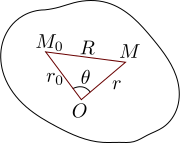
\includegraphics[width=0.3\textwidth]{figLejandr1.pdf}
\end{wrapfigure}
Пусть $r$ и $r_0$ -- радиусы векторы точек $M$ и $M_0$, a $\theta$ - угол между ними. 
Используя теорему косинусов представим $R$ через $r$
\[
    \frac{1}{R} = \frac{1}{\sqrt{r_0^2 + r^2 - 2 r r_0 \cos \theta}}
\]

Рассмотрим два случая
\begin{align*}
    &r > r_0 \quad \frac{r_0}{r} < 1 \quad \frac{r_0}{r} = \rho < 1\\
	&r < r_0 \quad \frac{r_0}{r} < 1 \quad \frac{r}{r_0} = \rho < 1
\end{align*}

\begin{align*}
    &1) \frac{1}{R} = \frac{1}{r \sqrt{1 + \rho^2 - 2 \rho \cos \theta}}\\
	&2) \frac{1}{R } = \frac{1}{r_0 \sqrt{1 + \rho^2 - 2 \rho \cos \theta}}
\end{align*}

\[ 
    \psi (\rho, \theta) = \frac{1}{\sqrt{1 + \rho^2 - 2 \rho \cos \theta}}
\]
Функция
\begin{equation}
    \psi(\rho, z) = \frac{1}{\sqrt{1 + \rho^2 - 2 \rho z}}
    \label{equ:poly}
\end{equation}
называется \textit{производящей функцией} полиномов Лежандра.
\begin{multline}
    \psi (\rho, z) = \left[1 + (\rho^2 - 2 \rho z) \right]^{-\frac{1}{2}} = 1 - \frac{1}{2} (\rho^2 - 2 \rho z) - \frac{1}{2} \left(- \frac{3}{2} \frac{1}{2}\right) (\rho^2 - 2 \rho z)^2 + \ldots = \\= 1 + z \rho + \left( \frac{3}{2}z^2 - \frac{1}{2}\right) + \rho^2 + \ldots
\end{multline}

Получим разложение функции $\psi$ в ряд.
\[
	\psi(\rho, z) = \left[1 + (\rho^2 - 2 \rho z) \right]^{- \frac{1}{2}} = \sum\limits_{n = 0}^{\infty} P_n (z) \rho^n
\]
\begin{equation}
    \psi(\rho, z) = \sum\limits_{n = 0}^{\infty} P_n (z) \rho^n
	\label{equ:polyRow}
\end{equation}
Коэффициенты разложения \eqref{equ:polyRow} при одинаковых степенях $\rho$ образуют \textit{полиномы Лежандра}.

Обратимся к формуле \eqref{equ:poly}
\[z = 1, \quad \psi (\rho, 1 )= (1 + \rho^2 - 2 \rho)^{- \frac{1}{2}} = (1 - \rho)^{-1} = 1 + \rho + \rho^2 + \ldots \Rightarrow P_n(1) = 1\]

В дальнейшем получим рекуррентное соотношение.
\subsubsection{Рекуррентные формулы}
Выведем три рекуррентные формулы.

Продифференциируем $\psi$ по $\rho$
\[
    \derp{\psi}{\rho}{} = \frac{2 \rho - 2 z}{2 (1 + \rho^2 - 2 \rho z)^{\frac{3}{2}}} = \frac{- (\rho - z)}{(1 + \rho^2 - 2 p z)^{\frac{3}{2}}}
\]
\begin{equation}
	(1 + \rho^2 - 2 \rho z) \derp{\psi}{\rho}{} = - (\rho - z) \psi
	\label{equ:poly3}
\end{equation}
Запишем формулу в виде степенного ряда относительно $\rho$, подставив в неё ряд \eqref{equ:polyRow}
\begin{multline*}
    (1 + \rho^2 - 2 \rho z) \left[\ldots + (n - 1) P_{n - 1} \rho^{n - 2} + n P_n \rho^{n - 1} + (n + 1) P_{n + 1} \rho^n + \ldots \right] = \\= - (\rho - z) \left(\ldots + P_{n - 1}\rho^{n - 1} + P_n \rho^n + P_{n + 1} \rho^{n + 1}+ \ldots \right)
\end{multline*}
Приведём подобные 
\[(n + 1) P_{n + 1} + (n - 1) P_{n - 1} - 2 n z P_n = - P_{n - 1} + z P_n\]
\[(n + 1) P_{n + 1} + n P_{n - 1} - (2n + 1) z P_n =0\]
Получим \textbf{первую} рекуррентную формулу
\begin{equation}
    (n + 1) P_{n + 1} - z(2n + 1) P_n + n P_{n - 1} = 0
	\label{equ:poly4}
\end{equation}

Продифференциируем $\psi$ по z.
\[
    \derp{\psi}{z}{} = \frac{\rho \psi}{(1 + \rho^2 - 2 \rho z)}
\]

\begin{equation}
    (1 + \rho^2 - 2 \rho z) \derp{\psi}{z}{} = \rho \psi
\end{equation}

\[
\begin{cases}
   \rho z \psi = z (1 + \rho^2 - 2 \rho z) \derp{\psi}{z}{}\\
   \rho^2 \psi = \rho (1 + \rho^2 - 2 \rho z) \derp{\psi}{z}{}
\end{cases}
\]

\[
    \rho \cancel{(1 + \rho^2 - 2 \rho z)} \derp{\psi}{\rho}{} = (z - \rho) \cancel{(1 + \rho^2 - 2 \rho z)} \derp{\psi}{z}{}
\]

\begin{equation}
    \rho \derp{\psi}{\rho}{} = (z - \rho) \derp{\psi}{z}{}
	\label{equ:poly6}
\end{equation}

В равенство \eqref{equ:poly6} подставляем выражение \eqref{equ:polyRow} 
\begin{multline*}
    \rho \left[\ldots + (n - 1) P_{n - 1} \rho^{n - 2} + n P_n \rho^{n - 1} + (n + 1) P_{n + 1} \rho^n + \ldots \right] =\\ = (z - \rho)\left[\ldots + P_{n - 1}' \rho^{n - 1} + P_n' \rho^n + P_{n +1}' \rho^{n + 1} + \ldots \right]
\end{multline*}
Получили \textbf{вторую} рекурентную формулу
\begin{equation}
    n P_n = zP_n' - P_{n - 1}'
	\label{equ:poly7}
\end{equation}
Имеется
\[
    \rho \derp{}{\rho}{} (\rho \psi) = \rho^2 \derp{\psi}{\rho}{} + \rho \psi
\]
\[
    \rho (\rho \psi) = \rho (z - \rho) \derp{\psi}{z}{} + (1 + \rho^2 - 2 \rho z) \derp{\psi}{z}{}
\]

Снова используем \eqref{equ:polyRow}.
\[
    \rho \psi = \rho (\ldots + P_{n - 1} \rho^{n - 1} + P_n \rho^n + P_n + \rho^{n + 1}) = \ldots + P_{n - 1} \rho^{n } P_n \rho^{n + 1} P_{n + 1}\rho^{n + 1}
\]
\[ 
    \derp{(\rho \psi)}{}{} = (\ldots + )
\]
\[
    \derp{\psi}{z}{} (\rho z - \rho^2+ 1 \rho^2 - 2 \rho z) = (1 \rho z) \derp{\psi}{z}{} = (1 - \rho z) (P_{n - 1}' \rho^{n - 1} + P_n' \rho^n + P_{n + 1}' \rho^{n+1} + \ldots)
\]
\[
    n P_{n - 1}\rho^n + (n + 1) P_n \rho^{n + 1} + (n + 2) P_{n + 1} \rho^{n + 2} = P_n' \rho^n - z P_{n - 1}' \rho^n + \ldots
\]
Получаем \textbf{третью} рекуррентную формулу
\begin{equation}
    n P_{n - 1} = P_n' - z P_{n - 1}'
	\label{equ:poly8}
\end{equation}
\subsubsection{Уравнение Лежандра}


%Для этого исключим из систем  \eqref{equ:poly7} и \eqref{equ:poly8} $P_{n - 1}$ и $P_{n - 1}'$. \\

%Сначала подставим $P_{n - 1}'$ из \eqref{equ:poly7} в \eqref{equ:poly8}
%\[
%   P_{n - 1}' = z P_n ' - n P_n
%\]
%\[
%    n P_{n -1 } = P_n ' - z \left[ z P_n ' - n P_n \right]
%\]
%\[
 %   n P_{n - 1} = (1 - z^2) P_n ' + n z P_n
%\]
%Затем продифференциируем последнее равенство по $z$ и ещё раз применим \eqref{equ:poly7} для $P_{n -1 }$
%\[
%    n P_{n - 1}' = - 2 z P_n' + (1 - z^2) P_n'' + n P_n + n z P_n '    
%\]
%\[
%    n (z P_n' - n P_n) = (n - 2) z P_n ' + (1 - z^2) P_n '' + n P_n
%\]
%\[
 %   (1 - z^2) P_{n}'' - 2 z P_n' + n(n + 1)P_n = 0
%\]
%Переобозначим
%\begin{equation}
 %   (1 - z^2) y'' - 2 z y' + n (n + 1)y =0
%	\label{equ:polyLejandr}
%\end{equation}
%Уравнение \eqref{equ:polyLejandr} называется полиномом Лежандра.\\
%Эквивалентная запись 
%\[
%    \der{}{z}{}\left[ (1 - z^2) \der{y}{z}{}\right] + n (n + 1) y = 0
%\]
\setcounter{equation}{0}
Найдём дифференциальное уравнение, решением которого явялется $P_n(z).$
%\begin{equation}
%	\der{}{z}{} \left[(1 - z^2) \der{y}{z}{} \right] + n(n + 1)y = 0
%	\label{equ:AttachedLajandr1}
%\end{equation}
%\[
%	y = P_n(z)
%\]
Реккурентные соотношения для полиномов Лежандра:
\begin{equation}
	(n + 1) P_{n + 1} (z) - z (2n + 1) P_n(z) + n P_{n - 1} (z) = 0
	\label{equ:AttachedLajandr2}
\end{equation}
\begin{equation}
	n P_n (z) - z P_n'(z) + P_{n - 1}(z) = 0
	\label{equ:AttachedLajandr3}
\end{equation}
\begin{equation}
	n P_{n - 1}(z) - P_n'(z) + z P_{n - 1}' (z) = 0
	\label{equ:AttachedLajandr4}
\end{equation}

\[
    \int\limits_{-1}^1 P_n(z) P_m (z) \, dz = 
	\begin{cases} 
		0 & n \neq m \\ 
		\frac{2}{2n + 1} & n = m 
	\end{cases}
\]
%\textit{при условии ограниченности}
%\begin{equation}
%	\abs{y (\pm 1)} < \infty.
%	\label{equ:AttachedLajandr2}
%\end{equation}

%\[
%    P_n(z) = \derp{y}{z}{n} = C \cdot \der{}{z}{n} [(z^2 - 1)^n]
%\]

Рассмотрим дифференциальную форму полиномов Лежандра:
\[
    y = (z^2 - 1)^n; \qquad \der{y}{z}{} = 2 n z (z^2 - 1)^n
\]

\[
    \der{y}{z}{}(z^2 - 1) - 2 n z y = 0
\]
Продифференциируем полученное уравнение $(n + 1)$ раз:
\[
    \der{}{z}{n + 1} \left[(z^2 - 1) \der{y}{z}{} - 2 n \der{}{z}{n + 1} (z y(z))\right] = 0
\]
\begin{align*}
	(u \cdot v)' &= u' v + u v'\\
	(u \cdot v)'' &= u'' c + 2 u' v' + v''\\
	(u \cdot v)''' &= u''' v + 3 u'' v' + 3 u' v '' + v'''
\end{align*}
Тогда 
\begin{equation}
	(u \cdot v)^n = u^{(n)} v + n u^{(n - 1)} v' + \frac{n(n - 1)}{2} u^{(n - 2)} + \ldots + u v^{(n)}
	\label{equ:AttachedLajandr5}
\end{equation}
\[
    \left[\der{}{z}{n + 2} (z^2 - 1) + (n + 1) \der{y}{z}{n+1} 2 z +n(n + 1) \der{y}{z}{n} \right] - 2 n \left[\der{y}{z}{n + 1} z + (n + 1) \der{y}{z}{n}  \right] = 0
\]

\[
    (z^2 - 1) \der{y}{z}{n + 2} + \der{y}{z}{n + 1} [\cancel{2 nz} + 2z - \cancel{2 nz}] + \der{y}{z}{n}[n^2 + n - 2n^2 - 2n] = 0
\]
\begin{equation}
	(1 - z^2) \der{y}{z}{n + 2} - 2 z \der{y}{z}{n + 1} + n(n + 1) \der{y}{z}{n} = 0
	\label{equ:AttachedLajandr6}
\end{equation}
Пусть $\der{y}{z}{n} = P_n$, тогда
\[
    (1 - z^2) \der{P_n}{z}{2} - 2 z \der{P_n}{z}{} + n(n + 1)P_n = 0
\]
Получили \textit{дифференциальное уравнение Лежандра}, которому удовлетворяет $P_n$:
\begin{equation}
    \der{}{z}{} \left[(1 -z^2) \der{P_n}{z}{} \right] + n (n + 1) P_n = 0
	\label{equ:equLejandr}
\end{equation}
где $P_n$ --- полиномы Лежандра:
\[
    P_n(z) = \der{y}{z}{n} = C \der{}{z}{n} \left[(z^2 - 1)^n \right]
\]
так как $y = (z^2 - 1)^n$, а по свойствам полиномов Лежандра $P_n(1) = 1$

\begin{align*}
    \der{}{z}{}\left[(z^2 - 1)^n \right] &= 2 z (z^2 - 1)^{n - 1} n\\
    \der{}{z}{2} \left[(z^2 - 1)^n \right] &= 2 n(z^2 - 1)^{n - 1} + 2 n (n - 1)z^2 (z^2 - 1)^{n - 2}\\
    \der{}{z}{n} \left[(z^2 - 1)^n \right] &= 2^n z^n n (n - 1)(n - 2) \ldots (z^2 - 1) + a(z^2 - 1) z^{n - 1} +b(z^2 - 1)^2 z^{n - 2}
\end{align*}
Тогда при $z = 1$
\[
    P_n(1) = C \der{}{z}{n} \left[ (z^2 - 1)^n \right] \bigl|_{z = 1} = C 2^n n! = 1
\]
и следовательно
\[
    C = \frac{1}{2^n n!}.
\]
Полиномы Лежандра можно представить в дифференциальной форме
\begin{equation}
    P_n(z) = \frac{1}{2^n n!} \der{}{z}{n} \left[(z^2 - 1)^n \right]
    \label{equ:Rodriger}
\end{equation}
Формула \eqref{equ:Rodriger} называется \textit{формулой Родригера.}\\
\subsubsection{Ортогональность полиномов Лежандра}\label{que:28}
Докажем ортогональность полиномов Лежандра на отрезке $[-1, 1]$

\begin{align*}
    &(1 - z^2) P_n'' - 2 z P_n + n (n + 1) P_n = 0 | P_m(z) dz\\
	&(1 - z^2) P_m'' - 2 z P_m + n (m + 1) P_m = 0 | P_n(z) dz
\end{align*}

\[
    \int\limits_{-1}^1 \left\{ P_m \der{}{z}{} \left((1 - z^2) \der{P_n}{z}{}\right) + n (n + 1) P_n P_m - P_n \der{}{z}{} \left((1 - z^2) \der{P_n}{z}{}\right) - m (m + 1) P_n P_m\right\} \, dz
\]
От первого и третьего слагаемого возьмём интеграл по частям

Если $n \neq m$ интеграл $= 0$
\[
    \int\limits_{-1}^1 P_n P_m \,dz = \begin{cases} 0 & n \neq m \\ \neq 0 & n = m \end{cases}
\]

\[
    P_n(z) = a_{nn} z^n + a_{n n - 1} z^{n - 2} + \ldots
\]
Полиномы Лежандра содержат только чётные, либо только нечётные коэффициенты степени $z$
\[
    P_{n-1}(z) = a_{n-1n-1} z^{n-1} + a_{n-1 n - 2} z^{n - 3} + \ldots
\]
Из равенства \eqref{equ:poly4} 
\[
    (n + 1) a_{n+1 n + 1} - (2 n + 1) a_{nn} = 0
\]

Теперь построим такую функцию
\[
    Q(z) = P_n(z) - \frac{a_{nn}}{a_{n - 1 n + 1}z P_{n - 1} (z)} = b_1 z^{n -2} + b_2 z^{n - 4} = \sum\limits_{n = 0}^{n - 2} b_n P_k(z)
\]

\begin{multline}
    N_n = \int\limits_{-1}^{1} P_n(z) P_n(z) \, dz = \int\limits_{-1}^1 P_n(z) \left(Q(z) + \frac{a_nn}{a_{n - 1}} z P_{n - 1}\right) \, dz = \\
	= \int\limits_{-1}^1 P_n Q (z) \, dz + \frac{a_nn}{a_{n - 1 n - 1}} \int\limits_{-1}^1 P_n z P_{n - 1} \, dz
\end{multline}

Воспользуемся равенством \eqref{equ:poly4}
\[
   z P_n = \frac{n P_{n - 1} + (n + 1) P_{n + 1}}{2n + 1}
\]
Получаем
\[
    N_n \int\limits_{-1}^1 P_n(z) P_n (z) \, dz = \frac{a_{nn}}{a_{n -1 n - 1}} \int\limits_{-1}^1 P_{n - 1} \left( \frac{n P_{n - 1} + (n + 1) P_{n + 1}}{2n + 1} \right)\, dz = \frac{a_{nn}}{ a_{n - 1 n - 1} \frac{n}{2 n + 1}} \int\limits_{-1}^1 P_{n - 1}^2 \, dz
\]

\[
    N_n = \frac{2 n - 1}{2 n + 1} N_{n - 1}
\]

\begin{align*}
    &N_0 = \int\limits_{-1}^1  dz = 2\\
    &N_1 = \int\limits_{-1}^1 z^2 dz = \frac{2}{3}\\
    &N_2 =  \frac{2}{5}\\
    &N_3 =  \frac{3}{7}
\end{align*}

По аналогии
\[
    N_n = \frac{2}{2 n + 1}
\]





 \newpage

	\subsection{Присоединённые функции Лежандра.}\label{que:29}
		\subsubsection{Присоединённые функции} \setcounter{equation}{0}
В задачах \textit{Штурма-Лиувилля} в многомерном случае уравнение Лежандра принимает вид
\begin{equation}
    \der{}{z}{} \left[ (1 - z^2) \der{y}{z}{} \right] +\left[n(n + 1) - \frac{m^2}{1 - z^2}\right] y = 0
		\label{equ:LejandrAtt1}
\end{equation}
где $m$ --- константа.

Будем искать решение $y$ в виде
\[
    y = (1 - z)^{\frac{m}{2}} v (z)
\]
Найдём первую производную
\[
    \der{y}{z}{} = \frac{m}{2} (1 - z^2)^{\frac{m - 2}{2}} (- 2 z) v + (1 - z^2)^{\frac{m}{2}} \der{v}{z}{}
\]
Умножим на $(1 - z^2)$
\[
    (1 + z^2) \der{y}{z}{} = - m z(1 - z^2)^{\frac{m}{2}} v + (1 - z^2)^{\frac{m + 2}{2}} \der{v}{z}{}
\]
\begin{multline*}
    \der{}{z}{} \left[ (1 -z^2) \der{y}{z}{} \right] = - m (1 - z^2)^{\frac{m}{2}} v + m \frac{m}{2} z (2 z) (1 - z^2)^{\frac{m - 2}{2}} v - mz(1 - z^2)^{\frac{m}{2}} \der{v}{}{} -\\ {}- \frac{m + 2}{2} (2 z) (1 - z^2)^{\frac{m}{2}} \der{v}{z}{} + (1 - z^2)^{\frac{m + 2}{2}} \der{v}{z}{2}
\end{multline*}
Подставим в формулу  \eqref{equ:LejandrAtt1}
\begin{multline*} 
    (1 - z^2)^{\frac{m + 2}{2}} \der{v}{z}{2} + \der{v}{z}{} \left[ - m z (1 - z^2)^\frac{m}{2} + (m + 2)z (1 - z^2)^\frac{m}{2} \right] +{}
	\\+ v \left[- m (1 - z^2)^\frac{m}{2} + m^2 z^2 (1 - z^2)^\frac{m - 2}{2} + n(n + 1)(1 - z^2)^2\frac{m}{2} - \frac{m^2}{1 - z^2} (1 - z^2)^\frac{m}{2} \right] = 0,
\end{multline*}
сократим на $(1 - z^2)^\frac{m}{2}$ 
\begin{equation}
    (1 -z^2) \der{v}{z}{2} - 2 z (m + 1) \der{v}{z}{} + \left[n(n + 1) - m(m + 1) \right] v = 0
	\label{equ:LejandrAtt2}
\end{equation}

Возьмём
\[
    (1 - z^2)\der{y^*}{z}{2} - 2 z \der{y^*}{z}{} + n(n + 1) y^* = 0, \qquad y^* = P_n(z)
\]
Возьмём первую производную\\
первое слагаемое
\[
    \der{}{z}{m} \left[(1 - z^2)\der{y^*}{z}{2} \right] = \der{y^*}{z}{m + 2} + m \der{y^*}{z}{m+1} (- 2 z) + \frac{m(m - 1)}{2} \der{y^*}{z}{m} (- 2) = 0
\]
второе слагаемое
\[
    \der{}{z}{m} \left[z \der{y^*}{z}{} \right] = \der{y^*}{z}{m + 1} z + m \der{y^*}{z}{m} 
\]

\begin{equation*}
	\der{y^*}{z}{m + 1} (- 2 z) + \frac{m(m + 1)}{2} \der{y^*}{z}{m} 
\end{equation*}

\begin{equation}
    (1 - z^2) \der{y^*}{z}{m + 2} - 2 z (m + 1) \der{y^*}{z}{m + 1} + \left[- m^2 + m - 2 m + n(n + 1) \right] \der{y^*}{z}{m} = 0
	\label{equ:LejandrAtt3}
\end{equation}

Если $v = \der{y^*}{z}{m}$, то \eqref{equ:LejandrAtt2} $=$ \eqref{equ:LejandrAtt3}
\[ 
	v = \der{y^*}{z}{m} = \der{}{z}{m} \left( P_n(m) \right)
\]
Подставив в уравнение \eqref{equ:LejandrAtt1}, получим решение
\begin{equation}
    y = (1 - z^2)^\frac{m}{2} \cdot \der{}{x}{m} P_n (z)= P_n^{(m)} (z)
	\label{equ:connLejandra}
\end{equation}
\eqref{equ:connLejandra} -- присоединённые полиномы Лежандра


\subsubsection{Ортогональность}\label{que:30}
Рассмотрим норму присоединённых полиномов Лежандра
\[
	N_{n, k}^{(m)} = \int\limits_{-1}^1 P_n^{(m)}(z)P_k^{(m)}(z)\, dz  =
	\begin{cases}
	    0 & n \neq k\\
		\neq 0 &n=k
	\end{cases}
\]

\[
    N_{n, k}^{(m)} = \int\limits_{-1}^1 (1 -z^2) \der{}{z}{m} (P_n) (1 - z^2)^\frac{m}{2} \der{}{z}{m} (P_k) \, dz = \int\limits_{-1}^1 \underbrace{(1 - z^2)^m \der{}{z}{m} P_n(z)}_\text{u} \cdot \underbrace{\der{}{z}{m} P_k(z)}_\text{dv} \, dz
\]
Интегрируем по частям
\begin{align*}
    &v = \der{}{z}{m - 1} P_k(z)\\
    &du = \der{}{z}{} \left[(1 - z^2)^m \der{}{z}{m} P_n(z) \right]
\end{align*}

%\begin{equation}
%    (1 - z^2) \derp{y}{z}{m+2} - 2 (m + 1) z \der{y}{z}{m+1} + \left[n(n + 1) - m(m + 1) \right] \der{y}{z}{m} = 0
%	\label{equ:ort1}
%\end{equation}

%\begin{equation}
%    P_n^{(m)} = (1 - z^2)^\frac{m}{2} \der{}{z}{m} P_n(z)
%	\label{equ:ort2}
%\end{equation}

\begin{multline*}
    \int\limits_{-1}^1 (1 - z^2)^m \der{}{z}{m} P_n(z) \der{}{z}{m}P_k(z) \,dz = \\ =\left. (1 - z^2)^m \der{}{z}{m} P_n (z) \der{}{z}{m - 1} P_k(z) \right|_{-1}^1 - \int\limits_{-1}^1 \der{}{z}{} \left[ (1 - z^2)^m \der{}{z}{m} P_n(z)\right] \der{P_k(z)}{z}{m - 1} \, dz
\end{multline*}
Оставшийся интеграл подставим в \eqref{equ:LejandrAtt3} и умножим на $(1 - z^2)$:
\[
	(1 - z^2)^m \der{}{y}{m + 2} - 2 (m + 1)z (1 - z^2)^m \der{}{y}{m + 1} + (1 - z^2)^m [n (n + 1) - m (m + 1)] \derp{y}{z}{m} = 0
\]

\begin{equation}
     \der{}{z}{} \left\{ (1 - z^2)^m \der{}{y}{m + 1} \right\} = - (1 - z^2)^m \left[ n(n + 1) - m(m +1) \right] \der{y}{z}{m}
	 \label{equ:ort3}
\end{equation}
Перепишем формулу \eqref{equ:ort3} $m = m' + 1 \Rightarrow m' = m - 1$

\begin{equation*}
     \der{}{z}{} \left\{ (1 - z^2)^m \der{}{y}{m} \right\} = - (1 - z^2)^{m-1} \left[ n(n + 1) - m(m - 1) \right] \der{y}{z}{m - 1}
\end{equation*}

\[
    n^2 + n - m^2 + m = (n + m) + (n^2 - m^2) = (n + m)(n - m + 1)
\]

\begin{multline*}
    N_{n,k}^{(m)} = \int\limits_{-1}^1 (1 - z^2)^{m} \der{}{z}{m} P_n(z ) \der{}{z}{m} P_k (z) \, dz =\\= \int\limits_{-1}^1 (1 - z^2)^{m - 1} \left[(n + m) (n - m + 1) \der{P_n(z)}{z}{m - 1}\right] \der{P_k(z)}{z}{m - 1}\, dz = \\ = [(n + m (n - m + 1))] \int\limits_{-1}
^1 (1 - z^2)^{m - 1} \der{}{z}{m - 1} P_n(z) \der{}{z}{m - 1} P_k(z) \, dz = \\ = [(n + m)(n - m + 1)]N_{n,k}^{(m - 1)} = (n + m) (n - m + 1) (n - m +2) N_{n, k}^{m - 2} = \\ = (n + m)(n + m - 1)\ldots (n + 1) (n - m + 1) (n - m + 2)\ldots n N_{n,k}^{(0)}
\end{multline*}
Вспомним определение факториала
\[
	n! = 1 \cdot 2 \cdot 3 \ldots n
\]
\[
   \frac{n(n - 1)(n + 2) \ldots (n - m + 2) (n - m + 1) (n - m) (n - m + 1)}{(n - m)(n - m - 1)} = \frac{n!}{(n - m)!}
\]

\[
    \frac{(n + m) ( \ldots) (n + 1) \ldots (n) (n - 1) \dots 1}{n (n - 1) \ldots 1} = \frac{(n + m)!}{n!} = \frac{n!}{(n - m)!}
\]
\[
	N_{n,k}^{(m)} = \frac{(n + m)! n!}{(n - m)!n!} N_{n, k}^{(0)}
\]
Окончательно получаем:
\begin{equation}
    N_{n,k}^{(m)} = \int\limits_{-1}^1 (1 - z^2)^m \der{}{z}{m} P_n(z) \der{}{z}{m} P_k (z) \, dz = \frac{(n + m)! }{(n - m)! } N_{n,k}^{(0)}
\end{equation}
Используя свойство ортогональности
\[
    \int\limits_{-1}^1 P_n^{(m)} (z) P_k^{(m)} \, dz = 
	\begin{cases}
	    0 &k \neq m\\
	\frac{2}{2n + 1} &k=m
	\end{cases}
\]
последнее равенство может быть представлено так:
\begin{equation}
    N_{n,k}^{(m)} = \frac{(n + m)! }{(n - m)! } \frac{2}{2n + 1}, \qquad \text{если}\quad m = k
\end{equation}
 \newpage

	\subsection{Гамма функция.}\label{que:33}
		\begin{equation}
    \Gamma(s + 1) = \int\limits_0^{\infty} e^{- x} x^s \, dx
	\label{equ:gamma_function}
\end{equation}


\begin{wrapfigure}{r}{0.4\textwidth}
	\centering
	\includegraphics[width=0.4\textwidth]{Gamma_plot.pdf}

\end{wrapfigure}


Функция \eqref{equ:gamma_function} -- гамма-функция.\\
\textbf{Свойства:}
\begin{itemize}
	\item $\displaystyle\Gamma(1 - s) \Gamma(s) = \frac{\pi}{\sin \pi s}$
	\item $\displaystyle\Gamma\left(\frac{1}{2} \right) = \sqrt{\pi}$
	\item $\displaystyle\Gamma(s + 1) = s \Gamma(s)$
	\item  $\displaystyle \Gamma'(x) = \psi(x) \Gamma(x)$ 
	%\item $\displaystyle B(x, y) = \frac{\Gamma(x) \Gamma(y)}{\Gamma(x + y)}$
\end{itemize}
Проинтегрируем по частям
\[
    \Gamma(s + 1) = - e^{-x} x^s |_0^{\infty} + \int\limits_0^{\infty} e^{-x} s x^{s - 1} \, dx = s \int\limits_0^{\infty} e^{-x} x ^{s - 1} \, dx
\]\\

\[
    \Gamma(1) = \int\limits_0^{\infty} e^{- x} x^0 \, dx = \int\limits_0^{\infty} e^{-x} \, dx = \left. e^{- x} \right|_0^{\infty} = 1
\]
\vspace{0.2in}
\[
    \Gamma \left(- \frac{1}{2} + 1\right) = \int\limits_0^{\infty} e^{-x} x^{- \frac{1}{2}} \, dx \left[ \begin{tabular}{c c} $x = z^2$ & $\sqrt{x} = z$\\ $dx = 2z dz$& \end{tabular} \right] = \int\limits_0^{\infty} \frac{e^{-z^2}}{z} 2 z \, dz = 2 \int\limits_0^{\infty} e^{-z^2} \, dz =\sqrt{\pi}
\]

\[
    \Gamma(1) = 1 \quad \Gamma\left(\frac{1}{2}\right) = \sqrt{\pi}
\]

\[
    \Gamma\left(\frac{3}{2}\right) = \Gamma\left(\frac{1}{2} + 1\right) = \frac{1}{2} \Gamma\left(\frac{1}{2}\right) = \frac{\sqrt{\pi}}{2}
\]

Гамма-функции встречаются в уравнениях Бесселя.



 \newpage

	\subsection{Сферические функции}\label{que:34}
		Сферические функции проще всего могут быть выведены при решении уравнения Лапласа для шаровой области методом разделения переменных (метод Фурье). \\
Мы рассмотрим вывод на примере решения задачи теплопроводности.

Будем искать решение уравнения в переменных $r, \theta, \varphi$
\[
    \derp{u}{t}{} = a^2 \left(\derp{u}{r}{2} + \frac{2}{r} \derp{u}{r}{} + \frac{1}{r^2 \sin \theta} \derp{}{\theta}{} \left(\sin \theta \derp{u}{\theta}{}\right) + \frac{1}{r^2 \sin^2 \theta} \derp{u}{\varphi}{2}\right)
\]

\begin{align*}
      &0 \leqslant r \leqslant R\\
	&0 \leqslant \theta \leqslant \pi\\
	&0 \leqslant \varphi \leqslant 2 \pi
\end{align*}



Связь с декартовой системой координат
\begin{align*}
      &x = r \sin \theta \cos \varphi\\
	&y = r \sin \theta \sin \varphi\\
	&z = r \cos \theta
\end{align*}
Положим 
\[
    u(t, r, \theta, \varphi) = T(t) v (r, \theta, \varphi)
\]
Решим задачу теплопроводности
\[
    T' v = a^2 T \Delta_{r, \theta \varphi} v \Big| \frac{1}{a^2 v T}
\]

\[
    \frac{T'}{a^2 T} = \frac{\Delta_{r, \theta, \varphi} v}{v} = - k^2
\]

\[
    \frac{T'}{a^2 T} = - k^2
\]

\[
    \Delta_{r, \theta  \varphi} v = - k^2 v
\]
$v(r, \theta, \varphi)$ будем искать в виде
\[
    v(r, \theta, \varphi) = R(r) Y(\theta, \varphi)
\]
Составим уравнение
\[
   \left. R'' Y + \frac{2}{r} R' + \left[\frac{1}{r^2 \sin v} \der{}{\theta}{} \left( \sin \theta \derp{Y}{\theta}{}\right)  + \frac{1}{r^2 \sin^2 \theta} \derp{Y}{\varphi}{2}\right]R(r) = - k^2 R Y \quad \right| \frac{r^2}{R Y}
\]

\[
    \frac{r^2 R'' + 2 r R'}{R} + k^2 r^2 = - \frac{\left[ \frac{1}{\sin \theta} \derp{}{\theta}{} \left( \sin \theta \derp{Y}{\theta}{} \right) + \frac{1}{\sin^2 \theta} \derp{Y}{\varphi}{2}\right]}{Y} = \lambda^2
\]


\begin{equation}
    R'' + \frac{2}{r} R' + \left(k^2 - \frac{\lambda^2}{r^2}\right) R = 0
	\label{equ:equBess}
\end{equation}
Уравнение \eqref{equ:equBess} сводится к уравнению Бесселя.

\[
    \derp{Y}{\theta}{2} + \ctg \theta \derp{Y}{\theta}{} + \frac{1}{\sin^2 \theta} \derp{Y}{\varphi}{2} + \lambda^2 Y = 0
\]
Решение задачи $Y(\theta, \varphi)$ также ищем методом разделения переменных
\[
    Y_\lambda = F(\varphi) P(\theta)
\]

\[
    \left. P'' F + \cos \theta P' F + \frac{1}{\sin^2 \theta} F'' P + \lambda^2 F P = 0\quad \right| \frac{\sin^2 \theta}{P F}
\]
Разделим переменные
\[
    \frac{\sin^2 \left[P'' + \cos \theta P' \right]}{P} + \lambda^2 \sin^2 \theta = - \frac{F''}{F} 
\]
В итоге получим
\[
    - \frac{F''}{F} = m^2 
\]
$m^2$ -- константа\\

$F$ удовлетворяет уравнению
\[ 
     F'' + m^2 F = 0
\]
%и условию переодичности
%\[
%    F(\varphi + 2 \pi) = F(\varphi)
%\]
Решается в виде
\[ 
     F = A_m \sin m \varphi + B_m \cos m \varphi
\]

\[
    \left. \sin^2 \theta P'' + \sin \theta \cos \theta (\lambda^2 \sin^2 \theta - m^2) P = 0 \quad \right|  Y_\lambda = F(\varphi) P(\theta)
\]
Замена
\[
    \cos \theta = z \quad \sin^2 \theta = (1 - z^2)
\]
Найдём производные
\begin{align*}
    &\der{P}{\theta}{} = \der{P}{z}{} \der{z}{\theta}{} = - \sin \theta \derp{P}{z}{}\\
    &\der{P}{\theta}{2} = - \cos \theta \der{P}{z}{} + \sin^2 \theta \der{P}{z}{2}
\end{align*}

\[
    P'' + \cos P' + \left(\lambda - \frac{m^2}{\sin^2 v} \right) P = 0
\]

\[
    (1 - z^2)P''_{zz} - \cos \theta \der{P}{z}{} + \cos \theta \left(- \sin \theta\right) \der{P}{z}{} + \left(\lambda - \frac{m^2}{1 - z^2}\right) P
\]

В итоге получили
\[
     (1 - z^2) \der{P}{z}{2} - 2 z \der{p}{z}{} + \left(\lambda - \frac{m^2}{1 - z^2} \right) P = 0
\]
 \newpage

\appendix
\label{appendix}
\section{Приложение}
	\subsection{Вопросы по курсу}
		
\begin{enumerate}
\setlength\parsep{0ex} 
\setstretch{0.0}
\setlength\itemsep{0ex} \small
\item Уравнение малых поперечных колебаний струны. c.~\pageref{que:1}\\
\item Уравнение теплопроводности. c.~\pageref{que:2}\\
\item Дифференциальные уравнения с двумя независимыми переменными. с.~\pageref{que:3}\\
\item Оператор Лапласа в декартовых, полярных, цилиндрических и сферических координатах. с.~\pageref{que:4}\\
\item Определения линейных, квазилинейных, однородных и неоднородных уравнений. с.~\pageref{que:5}\\
\item Классификация дифференциальных уравнений в частных производных второго порядка. с.~\pageref{que:6}\\
\item Приведение уравнений с двумя независимыми переменными к каноническому виду. с.~\pageref{que:7}\\
\item Постановка задачи Коши для волнового уравнения. Метод Даламбера для бесконечной струны. с.~\pageref{que:8}\\
\item Начальные и граничные условия для полубесконечной струны. Метод Даламбера для полубесконечной струны. с.~\pageref{que:9}\\
\item Метод разделения переменных или метод Фурье. Задача о колебаниях струны с закрепленными концами. с.~\pageref{que:10}\\
\item Метод разделения переменных или метод Фурье. Задача для гиперболического неоднородного уравнения с начальными и однородными граничными условиями. Функция влияния. с.~\pageref{que:11}\\
\item Редукция общей краевой задачи для волнового уравнения. с.~\pageref{que:12}\\
\item Определение сопряженных дифференциальных операторов. с.~\pageref{que:13}\\
\item Колебания прямоугольной пластины с начальными и однородными граничными условиями. с.~\pageref{que:14}\\
\item Задача Штурма-Лиувилля. Ортогональность собственных функций. с.~\pageref{que:15}\\
\item Метод Фурье в задаче Коши для уравнения параболического типа. с.~\pageref{que:16}\\
\item Фундаментальное решение уравнения теплопроводности. с.~\pageref{que:17}\\
\item Редукция общей задачи теплопроводности для конечного стержня. с.~\pageref{que:18}\\
\item Вывод формул Грина. с.~\pageref{que:19}\\
\item Фундаментальное решение уравнения Лапласа. с.~\pageref{que:20}\\
\item Принцип максимума уравнения Лапласа. с.~\pageref{que:21}\\
\item Единственность и устойчивость краевой задачи Дирихле для уравнения Лапласа.  с.~\pageref{que:22}\\
\item Задача Неймана для уравнения Лапласа. с.~\pageref{que:23}\\
\item Первая краевая задача для круга. с.~\pageref{que:24}\\
\item Метод функции Грина для задачи Дирихле в трехмерном случае. с.~\pageref{que:25}\\
\item Метод функции Грина для задачи Дирихле в двумерном случае. с.~\pageref{que:26}\\
\item Уравнение Лежандра. Полиномы Лежандра. с.~\pageref{que:27}\\
\item Ортогональность функций Лежандра. с.~\pageref{que:28}\\
\item Присоединенные функции Лежандра. с.~\pageref{que:29}\\
\item Ортогональность присоединенных функций Лежандра. с.~\pageref{que:30}\\
\item Уравнение Бесселя. Функции Бесселя. с.~\pageref{que:31}\\
\item Ортогональность Функций Бесселя. с.~\pageref{que:32}\\
\item Гамма функция. Основные свойства Гамма функции. с.~\pageref{que:33}\\
\item Разделение переменных в трехмерном уравнении Лапласа в сферических координатах. с.~\pageref{que:34}\\
\item Вариационная формулировка краевых задач. с.~\pageref{que:35}\\
\item Вариационный метод Ритца. с.~\pageref{que:36}\\
\end{enumerate}


\newpage
	\subsection{Оператор Лапласа}\label{que:4}
		Оперaтор Лапласа (лапласиан, оператор дельта) — дифференциальный оператор, действующий в линейном пространстве гладких функций и обозначаемый символом $\Delta$. 

Функции  $F$ он ставит в соответствие функцию
\[
	\left( \derp{}{x_1}{2} + \derp{}{x_2}{2} + \cdots + \derp{}{x_n}{2}   \right)F
\]

Оператор Лапласа эквивалентен последовательному взятию операций \href{http://en.wikipedia.org/wiki/Gradient}{градиента} и \href{http://en.wikipedia.org/wiki/Divergence}{дивергенции}: $\Delta~=~\mathrm{div}\,~\mathrm{grad}$, таким образом значение оператора Лапласа в точке может быть истолковано как плотность источников (стоков) потенциального векторного поля  в этой точке. В декартовой системе координат оператор Лапласа часто обозначается следующим образом \[\Delta = \nabla \cdot \nabla = \nabla^2,\] то есть в виде скалярного произведения оператора набла на себя.


\subsubsection*{Представления в различных системах координат}


\begin{flalign*}
	\begin{tabular}{l l l}
		Двумерное&&\\
		&\textbf{В декартовой} &$\displaystyle\Delta f = \derp{f}{x}{2} + \derp{f}{y}{2} $\\[12pt]
		&\textbf{В полярной} &$\displaystyle\Delta f = \frac{1}{r} \derp{}{r}{} \left( r \derp{f}{r}{}\right) + \frac{1}{r^2} \derp{f}{\theta}{2}$ \\[12pt]
		Трёхмерное&&\\
		&\textbf{В декартовой} &$\displaystyle\Delta f = \derp{f}{x}{2} + \derp{f}{y}{2} + \derp{f}{z}{2}$\\[12pt]
		&\textbf{В цилиндрической} &$\displaystyle\Delta f = \frac{1}{\rho} \derp{}{\rho}{} \left( \rho \derp{f}{\rho}{}\right) + \frac{1}{\rho^2} \derp{f}{\theta}{2} + \derp{f}{z}{2}$ \\[12pt]
		&\textbf{В сферической} &$\displaystyle\Delta f = \frac{1}{r^2} \derp{}{r}{} \left(r^2 \derp{f}{r}{} \right) + \frac{1}{r^2 \sin \varphi} \derp{}{\varphi}{} \left( \sin \varphi \derp{f}{\varphi}{}\right) + \frac{1}{r^2 \sin^2 \varphi} \derp{f}{\theta}{2}$\\
	\end{tabular}
\end{flalign*} \newpage
	\subsection{Линейные, квазилинейные, однородные и неоднородные уравнения}\label{que:5}
		Уравненение называется \textit{линейным}, если оно линейно как относительно старших производных $u_{xx}, u_{xy}, u_{yy}$, так и относительно функции $u$ и её первых производных $u_x$, $u_y$
\[
	a_{11} u_{xx} + 2 a_{12} u_{xy} + a_{22} u_{yy} + b_1 u_x + b_2 u_y + c u + f = 0
\]

Уравнение называется \textit{квазилинейным}, если коэффициенты $a, b, c$ зависят не только от $x$ и $y$, а являются, подобно $F$, функциями $x, y, z, u_x, u_y$.\\




Уравнение называется \textit{однородным}, если $f(x, y) = 0$.\\ \newpage
	\subsection{Сопряжённые дифференциальные операторы}\label{que:13}
		\begin{equation}
	\mathscr{L}[u] = u_{xx} - u_{yy}  + a u_x + b u_x + c u
	\label{equ:equDivOp}
\end{equation}
--- линейный дифференциальный оператор, соответствующий линейному уравнению гиперболического типа, а $a(x, y), b(x, y), c(x, y)$ --- дифференциируемые фукнции. Умножая $\mathscr{L}[u]$ на некоторую функцию $v$, запишем отдельные слагаемые в виде
\begin{align*}
	&v u_{xx} = (v u_x)_x - (v_x u)_x + u v_{xx}, &v b u_y &= (b v u)_y - u (bv)_y,\\
	&v u_{yy} = (v u_y)_y - (v_y u)_y + u v_{yy} &v c u &= u c v.\\
	&v au_x = (a v u)_x - u(a v)_x,
\end{align*}
Суммируя отдельные слагаемые, получаем:
\begin{equation}
	v \mathscr{L}[u] = u \mathscr{M}[v] + \derp{H}{x}{} + \derp{K}{y}{},
	\label{equ:equDivOp}
\end{equation}
где 
\[
	\mathscr{M}[v] = v_{xx} - v_{yy} - (a v)_x - (b v)_y + c v
\]
\begin{align*}
	&H = v u_x - v_x u + av u = (v u)_x - (2 u_x - a v) u = - (v u)_x + (2u_x + a u)v,\\
	&K= - v u_y + v_y u + b v u = -(v u)_y + (2v_y + b v) u = (u v)_y - (2 u_y - b y)v.
\end{align*}

Два дифференциальных оператора называются \textit{сопряжёнными}, если разность 
\[
	v \mathscr{L}[u] - u \mathscr{M}[v]
\]
является суммой частных производных по $x$ и $y$ от некоторых выражений $H$ и $K$. 

Рассматриваемые нами операторы $\mathscr{L}[u]$ и $\mathscr{M}[v]$, очевидно, являются \textit{сопряжёнными}.

Если $\mathscr{L}[u] = \mathscr{M}[u]$, то оператор $\mathscr{L}[u]$ называется \textit{самосопряжённым}.
 \newpage

\section{Примеры}
	\subsection{Задачи на метод Ритца}
		При изучении колебаний заделанного клина приходится исследовать функцию на экстремумы
\begin{example}{}
\[
I = \int\limits_0^1 (ax^3 y''^2- b x y^2)\, dx
\]

\begin{align*}
&y(1) = 0\\
&y'(1) = 0
\end{align*}

Координат функция удовлетворяет начальным условиям

\begin{align*}
(x &- 1)^2\\
(x &- 1)^2x\\
(x &- 1)^2x^3\\
&\ldots\\
(x &- 1)^2 x^{n-1}
\end{align*}
\[
y_n = \sum\limits_{k = 1}^n \alpha_k (x - 1)^2 x^{k - 1}
\]

\[
J_2 = (x - 1)^2(\alpha_1 + \alpha_2 \lambda)
\]

\[
J_2 = J(y_2) = \int\limits_0^1 \left[ ax^3 (6 \alpha_2x + 2 \alpha_1 - 6 \alpha_2)^2 -bx (x - 1)^n(\alpha_1 + \alpha_2 x) \right] \, dx
\]
Раскрыв скобки и проинтегрировав получим
\[
a \left[(\alpha_1-2\alpha_2)^2+\frac{24}{5}\alpha_2(\alpha_1 - 2 \alpha_2) + 6 \alpha_2 \right] - b\left[\frac{\alpha_1^2}{30} +2 \frac{\alpha_1\alpha_2}{105}+\frac{\alpha_2^2}{280} \right]
\]
Необходимое условие экстремума
\[
\derp{I_2}{\alpha_1}{} = 0 \quad \derp{I_2}{\alpha_2}{} = 0
\]

\[
\left(a - \frac{b}{30}\right)\alpha_1 + \left(\frac{2}{5} a - \frac{b}{105}\right) \alpha_2 = 0
\]

\[
\left(\frac{2}{5} a - \frac{b}{105}\right)\alpha_1 + \left(\frac{2}{5}a - \frac{b}{280}\right) \alpha_2 = 0
\]
Для получения колебаний необходиимо, чтобы был детерминант

\[
\begin{vmatrix} 
a - \dfrac{b}{30}& \dfrac{2}{5} a - \dfrac{b}{105}\\
\dfrac{2}{5} - \dfrac{b}{105}& \dfrac{2}{5}a - \dfrac{b}{280}
\end{vmatrix} = 0
\]
\[
\left(a - \frac{b}{30}\right) \left(\frac{2}{5}a - \frac{b}{280}\right)
\]
\end{example}
Здесь применяются вариационные методы.

\begin{enumerate}
\item Нужно подобрать функцию
\item Составить экстремум функции
\item Решить задачу
\end{enumerate}

\begin{example}{Найти экстремум функционала}

\[
I(y(x), z(x)) = \int\limits_0^{\frac{\pi}{2}} (y'^2 + z'^2 + 2 y z)\, dx
\]

\begin{align*}
y(0) &= 0\\
y\left(\frac{\pi}{2}\right) &= 1\\
z(0) &= 0\\
z\left(\frac{\pi}{2}\right) &= -1
\end{align*}

Система уравнений Эйлера имеет вид
\[
\begin{cases}
F_y- \der{}{x}{} F_y' = 0\\
F_z - \der{}{y}{} F_z' = 0
\end{cases}
\]

\[
\begin{cases}
z = y''\\
y - z'' = 0
\end{cases}
\]

\[
y = C_1 e^x + C_2 e^{-x} C_3 \cos x + C_4 \sin x
\]
Решение
\[
\begin{cases}
y = \sin x\\
z = - \sin x
\end{cases}
\]
\end{example}

\begin{example}{Исследовать на экстремум функционал}

\[
I(y,z) = \int\limits_0^1 (y'^2 + z'^2)\, dx
\]
Начальные условия
\begin{align*}
&y(0) = 0 \quad y(1) = 1\\
&z(0) = 0 \quad z(1) = 2
\end{align*}

\begin{align*}
&y'' = 0\\
&z'' = 0
\end{align*}

\[C_1 = 1 \quad C_3 = 2\]

\[
\begin{cases}
y = x\\
z = 2 x
\end{cases}
\]
Получили прямую

Исследуем на экстремумы
\begin{align*}
&F_{y'y'} = 2 \quad F_{y'z'} = 0\\
&F_{z'y'}=0 \quad F_{z'z'} = 2
\end{align*}

Усиленное условие Лежандра выполняется

\[ 
\begin{vmatrix} 
 2& 0 \\
0& 2
\end{vmatrix} = 4 > 0
\]
\end{example}
\begin{example}{Исследовать на экстремум функционал}

\[
I(y,z) = \int\limits_0^1 (y'^2 +z'^2 + 4 z)\, dz
\]

Начальные условия
\begin{align*}
&y(0) = 0 \quad y(1) = 1\\
&z(0) = 0 \quad z(1) = 0
\end{align*}

\[
\begin{cases}
y = x\\
z = x^2 - x
\end{cases}
\]

\[
\begin{vmatrix} 
 2& 0 \\
0& 2
\end{vmatrix} = 4 > 0
\]
\end{example}

\begin{example}{Исследовать на экстремум функционал}
\[
I(y) = \int\limits_0^2 (e^{y'} + 3)\, dx
\]
\end{example}	

\newpage
~
\thispagestyle{empty}
\vfill
\pagecolor[rgb]{0.8,0.8,0.8}
\hfill
\begin{figure}[t!]
\centering
\includegraphics[scale=0.4]{link.png}
\end{figure}
\begin{minipage}{10.5cm}

\textcolor[rgb]{0,0,0}{
\hrule height 0.5pt
\vspace{3pt}
Сборная солянка из материалов книги А.Н. Тихонов, А.А. Самарский <<Уравнения математической физики>> и курса лекций, прочитанного студентам потоку <<Прикладная математика и информатика>> СГАУ им. ак. С.П. Королёва в 2011 году. \\
%Лектор: доцент кафедры <<Прикладная математика>>, \mbox{Федечев А.Ф.} \\
%Компьютерная вёрстка: Проценко В.И.
}


\end{minipage}


\end{document}